% ═══════════════════════════════════════════════════════════════════
%  JOURNAL SUBMISSION EDITION — GENERATED FILE, DO NOT EDIT
%  Federated Solar-Flare Prediction on SWAN-SF: A Provenance, Leakage, and Evaluation-Protocol Audit
%  Regenerated programmatically from the repository record
%  (paper/) by tools/build_submission.py at v4.7, per Dossier
%  R-FS9-R6 register item 4. Every byte of the sections,
%  figures, and refs.bib is a verbatim copy of the record;
%  the only deviations are the declared transformations T1-T4
%  in that script. Re-run the generator after any paper/ change.
% ═══════════════════════════════════════════════════════════════════

\documentclass[11pt,a4paper]{article}

% ════════════════════════════════════════════════════════════════════
%  Federated Solar-Flare Prediction on SWAN-SF: A Benchmark Audit
%  of Provenance, Leakage, and Evaluation Protocols
%  (version-bearing strings live in tests/run_battery.py's
%  BATTERY_VERSION and the appendix history table only — R-FS9-R3 N2
%  lesson: hardcoded version markers in multiple places go stale)
%  arXiv-preprint-style single-column manuscript
% ════════════════════════════════════════════════════════════════════

\usepackage{graphicx}
\usepackage{xcolor}
\usepackage{geometry}
\usepackage{amsmath}
\usepackage{amssymb}

\geometry{a4paper, top=2.6cm, bottom=2.6cm, left=2.5cm, right=2.5cm}
% left and right margins are symmetric (iron rule)

\usepackage{booktabs}
\usepackage{tabularx}
\usepackage{longtable}
\usepackage{adjustbox}
\usepackage{enumitem}
\usepackage{caption}
\usepackage{microtype}
\usepackage{xurl}          % allow URLs to break at any character
\usepackage{placeins}   % \FloatBarrier at each section
\usepackage{needspace}

\captionsetup{font=small, labelfont=bf, skip=6pt}

% Bibliography: numeric citations, arXiv preprint style
\usepackage[numbers,sort&compress]{natbib}
\bibliographystyle{unsrtnat}

% hyperref ALWAYS last among content packages
\usepackage[
    colorlinks=true,
    linkcolor=blue!55!black,
    citecolor=blue!45!black,
    urlcolor=blue!55!black,
    bookmarks=true,
    bookmarksnumbered=true,
    unicode=true,
    pdftitle={Federated Solar-Flare Prediction on SWAN-SF: A Provenance,
              Leakage, and Evaluation-Protocol Audit},
    pdfauthor={Deepanshu Balhara, Davesh Vats},
    pdfsubject={Federated Learning, Solar Flare Prediction, Benchmark
                Audit, Space Weather},
    pdfkeywords={federated learning, solar flare prediction, SWAN-SF,
                 benchmark audit, data provenance, evaluation protocol,
                 BatchNorm, non-IID data, class imbalance}
]{hyperref}

% Orphan/widow prevention
\widowpenalty=10000
\clubpenalty=10000

% Allow emergency line stretching to avoid overfull boxes
\emergencystretch=1.8em

% Ragged-bottom: avoid stretched vertical glue
\raggedbottom

% Slight paragraph spacing for preprint readability
\setlength{\parindent}{1.2em}
\setlength{\parskip}{2pt plus 1pt}

% ── Custom math macros ──────────────────────────────────────────────
\newcommand{\R}{\mathbb{R}}
\newcommand{\E}{\mathbb{E}}
\newcommand{\w}{\mathbf{w}}
\newcommand{\norm}[1]{\left\lVert #1 \right\rVert}
\newcommand{\Fbeta}{F_{\beta}}

\title{Federated Solar-Flare Prediction on SWAN-SF: A Provenance, Leakage, and Evaluation-Protocol Audit}
\author{Deepanshu Balhara \and Davesh Vats}
\date{October 2026}


\begin{document}

\thispagestyle{plain}

\begin{center}
    {\color{black!85}\rule{\textwidth}{0.4pt}}\\[2.2em]
    {\LARGE\bfseries Federated Solar-Flare Prediction on SWAN-SF:\\[0.35em]
     A Provenance, Leakage, and\\[0.15em]
     Evaluation-Protocol Audit\par}
    \vspace{1.6em}
    {\large Deepanshu Balhara\textsuperscript{1} \quad and \quad
     Davesh Vats\textsuperscript{2}\par}
    \vspace{0.7em}
    {\small\textit{Independent Researchers}\textsuperscript{1,2}\par}
    % NOTE FOR AUTHORS: this file is GENERATED (tools/build_submission.py)
    % and byte-compared by the integrity battery — never hand-edit it.
    % To set institutional affiliations, edit this title block in the
    % generator and re-run `python tools/build_submission.py` (Dossier
    % R-FS9-R7, B13).
    \vspace{1.1em}
    {\small October 2026\par}
    \vspace{0.9em}
    {\footnotesize\textit{Journal submission edition — regenerated from the repository record (v4.7); source: \texttt{submission/src}, generator: \texttt{tools/build\_submission.py}}\par}
    \vspace{1.4em}
    {\color{black!85}\rule{\textwidth}{0.4pt}}
\end{center}

\vspace{0.4em}

\begin{center}
\begin{minipage}{0.92\textwidth}
\footnotesize
\textbf{Abstract ---}
We audit what happens when federated learning is evaluated on the
public SWAN-SF flare benchmark. Six \emph{simulated} clients hold
disjoint Dirichlet-skewed shards of the cleaned export under a frozen
protocol: immutable splits, validation-only selection and calibration,
a runtime leakage audit, and single-pass test evaluation. A provenance
audit against the raw benchmark (normalisation-invariant instance
matching, 98.7--100\% coverage, 100\% test-side label agreement) shows
the cleaned export's same-partition train/test pairing shares
instances: every flaring test window (6{,}234) also appears in
training, and 85.7--90\% of training positives are TimeGAN-synthetic.
On a leakage-free fold (training partitions 1--4, single-pass test on
partition 5) discrimination generalises for all arms (ROC-AUC
0.906--0.978) and the federated-versus-centralised gap disappears. A
BatchNorm-transport diagnostic then shows the in-partition FedAvg
collapse (test ROC-AUC 0.575) to be a composite evaluation artefact
--- untransported normalisation statistics, a mechanism documented in
the federated-learning literature since FedBN, compounded by a
saturated validation monitor and the checkpoint rule that monitor
feeds --- rather than a federated-learning failure: the same weights
score 0.951 with local statistics, and a controlled no-BatchNorm run
leaves both FedAvg and FedProx stable. On the raw, unbalanced substrate
the outcome is encoder-conditional (federated MLPs degrade; FedProx-LSTM
reaches ROC-AUC 0.970 and TSS 0.404). Calibration, not detection, is
the deployability
boundary: no validation-fit decision layer survives the prevalence
shift. Standard verification metrics (TSS, HSS, Brier skill,
persistence and climatology baselines, with reliability for the
in-partition arms) accompany every stored operating point of every
substrate; under the corrected persistence baselines, no arm beats
same-region label inertia (TSS 0.967) at this 24-hour label
geometry; on TSS, XGBoost (0.848) and logistic regression (0.489)
alone clear 24-hour-lagged persistence (0.418), and on HSS no arm
clears it (0.434). This is the first federated evaluation on
SWAN-SF and the first instance-level provenance audit of the cleaned
export; prior federated flare forecasting (Fu et al., 2023 preprint)
and prior random-split leakage warnings (the benchmark's own creators,
2019) both exist. Every number regenerates from committed artefacts
under a 20-file SHA-256-verified manifest.


\vspace{0.55em}
\noindent\textbf{Keywords:} federated learning; solar flare prediction;
SWAN-SF; benchmark audit; data provenance; evaluation protocol;
BatchNorm; non-IID data; class imbalance

\vspace{0.55em}
\noindent\footnotesize Source code and all experimental artefacts:
\url{https://github.com/Daveshvats/Federated-Learning-for-Distributed-Space-Weather-Monitoring}
\end{minipage}
\end{center}

\vspace{0.8em}


% ════════════════════════════════════════════════════════════════════
% SECTION 1 — INTRODUCTION
% ════════════════════════════════════════════════════════════════════
\section{Introduction}\label{sec:intro}

Solar-flare prediction from photospheric magnetogram time series is a
benchmark-driven machine-learning problem. The community's public
reference is SWAN-SF~\cite{angryk2020}, and the machine-learning
literature on it has grown around a small number of evaluation
conventions: randomised splits of pooled windows, the cleaned and
rebalanced export, and a reporting culture built on ROC/PR summary
statistics. Those conventions carry risk. The benchmark's own creators
warned that sliding-window temporal coherence ``invalidates the
randomness assumption, thus impacting all sampling practices''~\cite{angryk2019};
subsequent work has echoed the warning~\cite{ahmadzadeh2021}, and the
cleaned export's release paper explicitly prescribes pairing
temporally-preceding training partitions with a later test
partition~\cite{eskandari2024}. Machine-learning flare-prediction
models built on photospheric vector-magnetogram
summaries---the SHARP parameter suite~\cite{bobra2015} and its
descendants---have demonstrated statistically skilful classification of
flaring versus non-flaring active regions~\cite{leka2019,georgoulis2021};
the predictive signal lives in quantities such as total unsigned
current helicity, magnetic free energy, and flux-emergence proxies. What
has not existed, per the documented search protocol of
Section~\ref{sec:related}, is a federated treatment of SWAN-SF---with
its cleaned and raw substrates, its leakage structure, and its
centralised baselines---under an evaluation protocol that audits its own
benchmark artefacts.

Why federate a public benchmark whose data is, in reality, freely
poolable? Two honest reasons. Methodologically, cross-silo federated
learning~\cite{mcmahan2017,kairouz2021} is the standard instrument for
studying non-IID data heterogeneity under a controlled protocol: it
prescribes exactly what moves between data holders (model parameters)
and exactly what does not (raw observations), which makes it a clean
lens for asking how much of a benchmark's apparent difficulty survives
when the data is deliberately fragmented. Operationally, the
SHARP-style parameters at the centre of this pipeline are dominated by
a single public instrument (SDO/HMI via JSOC); the six-regional-agency
narrative sometimes attached to federated space-weather proposals does
not describe this data and is not claimed here. The six clients of
this study are a \emph{simulation protocol}---Dirichlet label skew
across disjoint shards---not a claim about any institution, and the
present study does not claim that any agency's flare data cannot be
pooled.

In cross-silo FL, each data-holder trains a shared architecture locally
and transmits model parameters to an aggregation server, which averages
them into a new global model; raw measurements do not move. FL has
proven transformative in medicine and digital health, where privacy
constraints really are binding~\cite{rieke2020}. Federated flare
forecasting itself is not new: Fu et al.\ posted a federated
transfer-learning preprint in July 2023 (Section~\ref{sec:related})
\cite{fu2023}. As a body of practice, FL also carries its own
evaluation-protocol hazards---statistics that travel with weights
(most visibly BatchNorm running moments, a failure mode documented
since FedBN~\cite{li2021fedbn}), drift monitors that saturate, and
checkpoint rules that quietly restore the wrong model---and a benchmark
audit is exactly the place to expose how those hazards interact with a
published comparison.

This paper provides that treatment, and its character is an audit: we
ask what a federated pipeline actually achieves on SWAN-SF, what the
benchmark's own artefacts do to the answer, and which parts of the
observed behaviour belong to the algorithms rather than to the
evaluation machinery. We present a complete, reproducible federated
framework---implemented, versioned, and released as open
source---that \emph{simulates} six clients (labelled A--F; no real
institution participates), each holding a non-IID shard of the
benchmark in both its cleaned/rebalanced form and its raw, naturally
imbalanced form, and evaluates whether federation can approach the
centralised upper bound without any data movement. The framework emits
M/X flare probabilities whose calibration, thresholds, and
false-alarm rates are themselves audited quantities in this paper---the
evaluation finds they do not survive the prevalence shift, and no
operational alerting claim is made. The downstream
flare$\to$CME$\to$storm$\to$GIC chain is physically far from the
quantity modelled here and is not evaluated
(Section~\ref{sec:limitations}; see \cite{boteler2019} for that
literature). The specific contributions are:

\begin{enumerate}[leftmargin=2em, itemsep=3pt]
  \item \textbf{A problem formulation and system architecture} that maps
  flare-probability estimation onto a cross-silo federated
  classification problem with a safety-critical, recall-weighted
  objective, and that operationalises client heterogeneity as a
  concrete, simulable protocol (Section~\ref{sec:problem} and
  Section~\ref{sec:method}).
  \item \textbf{A non-IID federation protocol for SWAN-SF} that combines
  Dirichlet label-skew partitioning across six simulated regional
  clients, a server-aware Fed-Focal loss \cite{sarkar2020} for extreme
  class imbalance, and optional distribution-aware aggregation and
  per-client SMOTE oversampling (both studied as ablation arms; SMOTE
  is inert on the cleaned variant and an executed negative at natural
  prevalence), on top of FedAvg
  \cite{mcmahan2017}, FedProx \cite{li2020}, and SCAFFOLD
  \cite{karimireddy2020} training loops
  (Section~\ref{sec:method}).
  \item \textbf{A frozen, leakage-audited evaluation protocol and a
  data-provenance audit of the benchmark export.} The protocol
  comprises an immutable train/validation/test contract, calibration
  and threshold selection on validation only, single-pass test
  evaluation, a centralised-MLP architecture control, five-seed
  statistics, a 24-cell component-ablation grid, region-disjoint
  split generation, natural-prevalence operating points, untouched
  client holdouts, a training-budget audit, event-level alerting
  metrics, and a calibration-comparison harness
  (Section~\ref{sec:experiments}). The provenance audit aligns every
  cleaned window to the raw SWAN-SF instances (Harvard Dataverse;
  normalization-invariant matching) and finds that the cleaned
  export's same-partition train/test pairing shares instances---including 100\% of the flaring test windows and 85.7--90\%
  TimeGAN-synthetic training positives---so the study re-evaluates all
  headline claims on a leakage-free temporally-preceding fold
  (Section~\ref{sec:provenance}). The leakage phenomenon itself is
  documented prior art---the benchmark's creators warned about
  random-split overlap in 2019~\cite{angryk2019} and the cleaned
  export's release prescribes temporally-preceding
  folds~\cite{eskandari2024}; what is new here is the instance-level
  quantification, performed inside a federated study.
  \item \textbf{A leakage-free federated evaluation.} On the
  temporally-preceding fold (training partitions 1--4, single-pass
  test on partition 5, natural 1.31\% prevalence), all arms
  generalise (ROC-AUC 0.906--0.978); the in-partition
  federated-versus-centralised gap disappears (FedProx 0.976/0.308
  vs architecture-matched centralised MLP 0.973/0.382); the
  threshold-transfer and calibration failures persist; and an
  event-level evaluation on 65 physical M/X-class events shows
  detection is not the deployability boundary---XGBoost's false-alarm
  burden is roughly $7\times$ lower than every neural arm's
  (Section~\ref{sec:res-leakfree}).
  \item \textbf{A raw-substrate re-execution and the encoder-conditional
  collapse.} Retraining the identical frozen protocol on the raw,
  unbalanced benchmark (natural prevalence, no synthetic positives, the
  release's imputation and normalisation reproduced in-pipeline with
  train-only parameters) separates the arms decisively: every
  federated \emph{MLP} arm degrades sharply (FedAvg detects zero of 65
  events; SCAFFOLD 0.768/0.057) while the same protocol with the
  sequential SolarLSTM restores the federated standing (FedProx-LSTM
  0.970/0.404; SCAFFOLD-LSTM the substrate's highest event-level
  detection, 55/65 at 0.4 false-alarm windows per day --- an
  implementation-case result, since the arm runs as the sign-inverted,
  cold-start variant disclosed in Section~\ref{sec:method}), a second seed
  holds all four sequence arms within $\pm$0.005 ROC-AUC, and
  per-client SMOTE at natural prevalence is a clean negative---so the
  balanced-substrate standing is a property of the flattened-feature
  MLP, not of federation per se (Sections~\ref{sec:res-raw}--\ref{sec:res-lstmrep}).
  \item \textbf{A BatchNorm-transport diagnostic and a controlled
  no-BatchNorm experiment, which re-attribute the in-partition
  FedAvg-versus-FedProx gap.} The underlying mechanism---weight
  averaging without normalisation statistics---is established
  knowledge in the FL literature since FedBN~\cite{li2021fedbn} and
  its successors~\cite{wang2023bn,guerraoui2024bn,bnscaffold2024};
  the contribution here is the composite failure-mode dissection on
  this pipeline and the self-correction of our own earlier artefact.
  The shipped implementation transports
  model parameters only, so BatchNorm running statistics remain at
  initialisation on the server for the entire run; under that
  evaluation the FedAvg global model drifts from 0.950 to 0.098 test
  ROC-AUC over 50 rounds, and a saturated validation monitor ($F_1
  = 2p/(1{+}p)$ whenever every prediction is positive) restores the
  collapsed round-20 checkpoint as the ``best'' model. The same
  weights score 0.951 under correct normalisation and 0.953 even at
  round 50; with BatchNorm layers removed, both FedAvg and FedProx
  train stably to near-identical test quality, so the published
  algorithm gap is substantially an evaluation-implementation
  artefact (Sections~\ref{sec:res-bn}--\ref{sec:res-nobn}).
  \item \textbf{An in-partition data-locality study, disclosed as
  such.} On the same-partition protocol (331{,}185 test windows,
  1.88\% prevalence) whose instance overlap the audit quantified,
  FedProx attains ROC-AUC 0.954 (97.7\% of the XGBoost reference's
  0.977) against the architecture-matched centralised MLP's 0.888, a
  comparison whose optimisation budgets are documented and
  budget-matched; these numbers are retained as protocol-stability
  evidence with the corrected attribution above, not as
  generalisation estimates (Section~\ref{sec:results}).
  \item \textbf{A cross-model interpretability audit.} SHAP analysis
  of both the centralised XGBoost reference and the federated global
  model, with physical-parameter-group aggregation, shows both
  concentrate decisions on current helicity, the Schrijver
  flux-emergence proxy \cite{schrijver2007}, and Lorentz-force
  components---consistent with established flare physics
  (Section~\ref{sec:results}).
\end{enumerate}

We are explicit about what is \emph{not} claimed: per-client SMOTE
contributes nothing on either substrate (zero synthetic samples on
the cleaned variant; an executed negative at natural prevalence); the
transport protocol moves full model weights, not data, and confers no
cryptographic privacy (the secure-aggregation sketch verifies
arithmetic cancellation only); the six clients are simulated, not real
agencies; and the downstream flare$\to$CME$\to$storm$\to$GIC chain
is discussed as a boundary, not evaluated.

The released framework also carries a documented revision history
(Appendix~\ref{sec:appendix}): a multi-version stability iteration in
which Dirichlet concentration, focal-loss alpha clamping, optimiser
choice, and dataset auditing were each adjusted in response to
diagnosed failure modes, and the audit findings reported here.
We keep that record because reproducible failure diagnosis is
transferable know-how for first FL deployments in the physical
sciences.

The remainder of the paper is organised as follows.
Section~\ref{sec:related} reviews flare prediction and federated
learning. Section~\ref{sec:problem} formalises the problem.
Section~\ref{sec:method} details the system architecture and
methodology. Section~\ref{sec:experiments} describes the experimental
setup, Section~\ref{sec:results} presents and analyses results, and
Section~\ref{sec:discussion} discusses operational integration and
engineering lessons. Section~\ref{sec:limitations} states limitations
and future work, and Section~\ref{sec:conclusion} concludes.

% ════════════════════════════════════════════════════════════════════
% SECTION 2 — BACKGROUND AND RELATED WORK
% ════════════════════════════════════════════════════════════════════
\section{Background and Related Work}\label{sec:related}

\subsection{Solar flare prediction from photospheric magnetograms}

The physical premise of data-driven flare forecasting is that the
photospheric magnetic field of an active region encodes the stress
budget that a future flare will release. Schrijver~\cite{schrijver2007}
demonstrated that a single scalar---the R-value, the unsigned flux
within high-gradient polarity-separation corridors---separates
major-flaring regions from non-flaring ones with striking reliability,
and this proxy remains among the strongest single flare predictors
identified to date. Bobra and Couvidat~\cite{bobra2015} operationalised
the machine-learning view of the problem, showing that a support-vector
machine trained on 25~SHARP parameters derived from SDO/HMI vector
magnetograms can forecast M-class flares with useful skill, and that
feature selection matters as much as model choice. Subsequent
community-wide blind tests, most notably the multi-method comparison of
Leka et al.~\cite{leka2019}, established two durable findings: (i)~no
single method dominates across all event definitions and skill
metrics, and (ii)~the effective ceiling on skill is set by the quality
and homogeneity of the training data rather than by classifier
complexity.

The European FLARECAST project~\cite{georgoulis2021} pushed the
operational agenda further, combining multiple forecasting methods and
data sources in an open framework, and it explicitly confronted the
data-heterogeneity problem that motivates the present paper. On the
data side, the SWAN-SF benchmark of Angryk et
al.~\cite{angryk2020} released a multivariate time-series dataset of
4{,}098 active-region (MVTS) tracks with 24 physical parameters per
timestep and flare-history labels, specifically designed to make flare
prediction reproducible and comparable; it has since become the
community's reference benchmark, and a family of cleaned and rebalanced
variants (random undersampling, Tomek-link cleaning, and TimeGAN-based
synthetic augmentation \cite{yoon2019}) has been curated to make the
benchmark tractable for supervised learning. Recent deep-learning work
on SWAN-SF continues to raise the centralised ceiling: contrastive
pretraining and multifaceted preprocessing \cite{eskandari2024} and
LSTM-style temporal architectures \cite{hassani2025} exploit the
sequential structure of the 60-minute observation windows. All of these
works, without exception, assume that the full training corpus is
available in one place.

\subsection{Federated learning under statistical heterogeneity}

Federated learning was introduced by McMahan et
al.~\cite{mcmahan2017} in the FedAvg formulation: clients perform
several epochs of local SGD on private data, and a server aggregates
the resulting weights by sample-size-weighted averaging. The defining
difficulty, identified almost immediately, is statistical
heterogeneity: when client data distributions differ---the non-IID
setting---local optima diverge from the global optimum, and naive
averaging can oscillate or diverge \cite{zhao2018}. FedProx
\cite{li2020} addresses this by adding a proximal term
$(\mu/2)\norm{\w-\w^{(t)}}^{2}$ to each client's local objective that
anchors local training to the current global model, tolerating partial
work and heterogeneous local computation. SCAFFOLD \cite{karimireddy2020}
attacks the same problem with control variates that correct client
drift using variance reduction. The comprehensive survey of Kairouz et
al.~\cite{kairouz2021} situates these algorithms within the broader
open-problem landscape, including robust aggregation, personalisation,
and privacy. Cross-silo FL---few, reliable, institutionally owned
clients---is the deployment regime relevant to space-weather agencies,
and it contrasts with the cross-device regime in its stability
requirements and long-lived participants.

A distinct and, for this study, decisive strand concerns normalisation
statistics under heterogeneity. FedBN~\cite{li2021fedbn} established
that BatchNorm running statistics are a per-client feature that
weight-averaged federation must \emph{not} naively transport, and that
keeping them local outperforms both FedAvg and FedProx under feature
shift. Wang et al.~\cite{wang2023bn} supplied the convergence analysis
of exactly this mismatch, Guerraoui et al.~\cite{guerraoui2024bn}
showed corrected statistics restore centralised-level evaluation
performance, and BN-SCAFFOLD~\cite{bnscaffold2024} documents BN drift
crippling SCAFFOLD specifically. The parameters-only transport bug we
diagnose in Section~\ref{sec:res-bn} is an engineering-level
instantiation of this literature's central mechanism --- the mechanism
is textbook; the composite failure chain (initialised-buffer evaluation
times a saturated monitor times a checkpoint rule) is the
pipeline-specific part.

\subsection{Class imbalance in federated learning}

Flare prediction inherits an extreme class-imbalance regime: in
SWAN-SF's natural test distribution, roughly 1.9\% of windows precede
M/X-class flares, while the rebalanced training partitions sit near
parity. The focal loss of Lin et al.~\cite{lin2017}, originally
developed for dense object detection, down-weights easy examples with a
$(1-p_t)^{\gamma}$ modulating factor and concentrates gradient on hard
positives; it has become the default imbalance workhorse. Sarkar et
al.~\cite{sarkar2020} adapted focal loss specifically to FL in the
Fed-Focal formulation, in which the class-weighting parameter is
adjusted using information available at the server about the global
class distribution, so that clients with different local positivity
rates do not implicitly reweight the global objective. In parallel,
synthetic oversampling remains a standard pre-processing response:
SMOTE \cite{chawla2002} interpolates minority-class neighbours, and
mixup \cite{zhang2018} creates convex combinations of training pairs.
Under federation, rebalancing must be applied locally per client, since
the pooled distribution is precisely what no participant can inspect.

\subsection{Positioning of this work and search protocol}
\label{sec:litsearch}

Two research threads---physics-grounded flare prediction and
heterogeneity-robust federated learning---have developed largely
independently, and one prior work joins them: Fu, Wan, Huang, Han, and
Peng posted ``Federated Transfer Learning for Soalr Flare Forecasting''
[title sic] to Research Square on 10~July~2023, formatted for
\emph{Solar Physics}~\cite{fu2023}. That preprint applies federated
transfer learning to flare forecasting on its own data substrate; it
remains unrefereed, and we found no evidence of formal journal
publication as of this revision. It does not evaluate SWAN-SF, reports
no provenance audit, and, to our knowledge, no follow-up has appeared.
We note that its evaluation protocol---a random 7:1.5:1.5 split of
pooled windows (AUC 0.936 on the Tianchi flare dataset)---is precisely
the random-split convention whose instance-sharing risk this paper
quantifies for SWAN-SF; the comparison is offered as context, not as a
score comparison across datasets.
Because novelty claims are factual statements about the literature, we
document the search protocol behind ours rather than relying on ``to
the best of our knowledge''. The search was last
repeated on 29~September 2026 across general web, arXiv, NASA ADS,
and publisher indexes (ScienceDirect, IEEE) reached through a web
search engine, using four query strings: (i)~\emph{federated learning
solar flare prediction}; (ii)~\emph{federated learning space weather
forecasting}; (iii)~\emph{federated learning SWAN-SF benchmark
magnetogram}; (iv)~\emph{cross-silo federated learning geophysics
heliophysics distributed observatories}. Records were included if
they apply federated or distributed multi-client learning without raw
data pooling to flare prediction or space-weather forecasting; records
were excluded if they concern centralised machine learning for flares
(the case for all entries of query~i), federated forecasting of
\emph{solar power or irradiance}, federated \emph{terrestrial}
weather forecasting, or federated computing on spacecraft without a
scientific forecasting task (the categories returned by query~ii).
Screening the 30 records returned by the four queries yielded
\emph{zero} in-scope records; the raw result listings are committed
with the repository (\texttt{docs/lit\_search/}, each listing
embedding its query date since v4.6). That screening
\emph{missed} the Fu et al.\ preprint above---exactly the
grey-literature coverage limitation this section flags---and the
preprint surfaced only in a targeted verification pass during the
present revision. We note two further limitations of this protocol:
web-engine coverage of preprint servers is incomplete, and the
screening was single-reviewer, so a PRISMA-style dual-screened log
remains queued repository work. Three facts bound the novelty claim honestly. The leakage
phenomenon is documented prior art: the SWAN-SF creators warned that
temporal coherence invalidates randomised
sampling~\cite{angryk2019}, Ahmadzadeh et al.\ repeated the
warning~\cite{ahmadzadeh2021}, and the cleaned export's release paper
prescribes temporally-preceding folds~\cite{eskandari2024}; the
BatchNorm-transport mechanism is textbook since
FedBN~\cite{li2021fedbn}. Within those limits, the present work is
the first federated evaluation on the SWAN-SF benchmark (in both
its cleaned and raw substrates, against centralised baselines of
matched architecture), the first \emph{instance-level} provenance
audit of the cleaned export (normalisation-invariant matching of
every window to the raw benchmark), and the first leakage-free
re-evaluation of federated flare prediction under the benchmark's
intended protocol. It also contributes a rarely documented artifact:
an honest engineering log of the failure modes encountered when FL
meets a severely imbalanced physical-science benchmark
(Appendix~\ref{sec:appendix}).

% ════════════════════════════════════════════════════════════════════
% SECTION 3 — PROBLEM FORMULATION
% ════════════════════════════════════════════════════════════════════
\section{Problem Formulation}\label{sec:problem}

\subsection{Federated risk minimisation}

Let $K$ denote the number of participating clients (simulated shards
of the pooled benchmark), each
holding a private dataset
$\mathcal{D}_k = \{(x_i, y_i)\}_{i=1}^{n_k}$ of active-region
observation windows $x_i \in \R^{d}$ and binary labels
$y_i \in \{0,1\}$ indicating whether an M- or X-class flare occurs
within the forecasting horizon. Let
$\mathcal{D} = \bigcup_{k=1}^{K} \mathcal{D}_k$ with
$n = \sum_k n_k$. The goal of standard centralised learning is to
solve
\begin{equation}\label{eq:central}
    \min_{\w \in \R^{p}} \;
    F(\w) \;=\; \frac{1}{n}\sum_{i=1}^{n}
    \ell\big(f_{\w}(x_i),\, y_i\big),
\end{equation}
where $f_{\w}$ is the prediction model, $\ell$ a per-sample loss, and
$p$ the number of parameters. In the federated setting this objective
is decomposed as a weighted sum of local empirical risks
\begin{equation}\label{eq:fedobj}
    \min_{\w} \; F(\w) \;=\; \sum_{k=1}^{K} \rho_k \, F_k(\w),
    \qquad
    F_k(\w) \;=\; \frac{1}{n_k}\sum_{(x_i,y_i)\in\mathcal{D}_k}
    \ell\big(f_{\w}(x_i),\, y_i\big),
\end{equation}
with aggregation weights $\rho_k \ge 0$, $\sum_k \rho_k = 1$. The
vanilla FedAvg choice is $\rho_k = n_k / n$; Section~\ref{sec:method}
describes the distribution-aware weights used in this work.

\subsection{The data-locality constraint}

The operational constraint that distinguishes cross-silo FL from
distributed optimisation is not an algorithmic preference but an
institutional invariant: for every round $t$ and client $k$, the
server may observe only the weight increment
$\Delta \w_k^{(t)} = \w_k^{(t+1)} - \w^{(t)}$ (or equivalently the
locally trained weights), never $x_i$ or $y_i$ for any sample in
$\mathcal{D}_k$. Formally, the communication transcript
\begin{equation}\label{eq:privacy}
    \mathcal{T} \;=\;
    \big\{\Delta \w_k^{(t)}\big\}_{k=1,\dots,K;\; t=1,\dots,T}
\end{equation}
is the only quantity that crosses the client boundary. This is the
data-locality constraint that motivates cross-silo federated learning
in settings where shards genuinely cannot be pooled---proprietary
archives, cross-border data governance, organisational silos. We
stress that no such constraint binds this benchmark: the SWAN-SF
data is public and freely poolable, and the federated protocol here
is a controlled simulation of the constraint, not a response to it.
The released framework nonetheless enforces the property by
construction: the client-side pipeline never serialises raw shards.
We further stress the scope of the property: it is
\emph{data locality}, not cryptographic privacy. The transcript
$\mathcal{T}$ itself can leak information about training data
(Section~\ref{sec:threatmodel}); defending against an adversary who
observes it requires secure aggregation or differential privacy, which
are implemented but not evaluated for accuracy cost here.

\subsection{Statistical heterogeneity}

In genuine cross-silo deployments, participating organisations sample
different populations under different label distributions, so the
local class priors $p_k = \Pr(y=1 \mid k)$ differ from the pooled
prior $\bar{p}$ --- statistical heterogeneity, the defining
difficulty of federated optimisation. Because SWAN-SF is a
single-instrument, whole-disk benchmark, no physical mechanism
produces such skew here; we therefore \emph{impose} it by
partitioning the pooled training data among $K$ clients with a
symmetric Dirichlet distribution of concentration $\alpha$
(Section~\ref{sec:method}),
so that the realised local priors span a wide range around $\bar{p}$.
The partition is a simulation instrument --- a test of federation
under heterogeneity, not a claim about how the data is produced: the
labels and windows come from one observatory pipeline for every
shard. The consequence for optimisation is well documented
\cite{zhao2018,li2020}: local objectives $F_k$ become misaligned, and
plain averaging of locally optimised weights introduces drift that
grows with the number of local epochs. FedProx counteracts this drift
by locally solving
\begin{equation}\label{eq:fedprox}
    \min_{\w} \;
    F_k(\w) \;+\; \frac{\mu}{2}\,\norm{\w - \w^{(t)}}^{2},
\end{equation}
which keeps client updates in a trust region around the global model.
The strength of this anchor, $\mu$, is a central hyperparameter of
this study.

\subsection{A safety-critical, recall-weighted objective}

Rare-event forecasting inverts the usual classification cost
structure: at 1--2\% positive prevalence an all-clear forecast is
98--99\% accurate and useless, while a missed positive is the event
the forecast exists to catch. Following rare-event evaluation
practice, we therefore evaluate with the $F_\beta$ measure
\begin{equation}\label{eq:fbeta}
    \Fbeta \;=\;
    \frac{(1+\beta^{2})\, P\, R}{\beta^{2} P + R},
    \qquad \beta = 2,
\end{equation}
where $P$ and $R$ are precision and recall; $\beta = 2$ weights recall
twice as heavily as precision. Because the deployed decision rule is a
threshold $\tau$ on the predicted flare probability, the framework
treats $\tau$ as a free, per-model parameter selected on held-out
validation evidence to maximise Eq.~\eqref{eq:fbeta}, rather than
fixing $\tau = 0.5$ by convention. Section~\ref{sec:results} shows this
choice is not cosmetic: at the conventional threshold, every federated
model trained on rebalanced local data is operationally unusable, and
threshold optimisation is what converts a well-ranked model into a
usable detector.

% ════════════════════════════════════════════════════════════════════
% SECTION 4 — SYSTEM ARCHITECTURE AND METHODOLOGY
% ════════════════════════════════════════════════════════════════════
\section{System Architecture and Methodology}\label{sec:method}

\subsection{Architecture overview}

\begin{sloppypar}
Figure~\ref{fig:arch} shows the complete system. Six simulated
clients---labelled neutrally A--F (plain identifiers; the labels
carry no geographic or institutional mapping, and no real institution
participates in this study)---each hold a private, non-IID shard of the
benchmark. In every communication round, each selected
client trains a local copy of the shared model on its shard (with an
imbalance-robust loss, described below), and transmits its model
parameters to the aggregation server (the implementation transports
full weight tensors both directions; delta/weight-increment encoding
and quantised uplinks are the communication-cost model's future
compression path, not what the code does). The server forms the next global
model by size-weighted averaging, broadcasts it to all clients, and
the cycle repeats for $T = 50$ rounds. Downstream of federation, the
global model emits flare probabilities; the evaluation of this paper
finds that its calibration and frozen operating points do not survive
the prevalence shift, so no alerting claim is made. Any downstream
use---CME propagation and storm forecasting, geomagnetic-hazard
estimation, GIC and power-system response modelling---would require
components this paper does not evaluate, and the
flare$\to$CME$\to$storm$\to$GIC chain is far from the quantity
modelled here (Section~\ref{sec:limitations}). The division of labour
is deliberate: everything that touches raw magnetogram data (loading,
local training) executes inside the client boundary; everything the
server touches is a weight tensor.
\end{sloppypar}

\begin{figure}[t]
    \centering
    \begin{adjustbox}{max width=\textwidth, max height=0.46\textheight}
        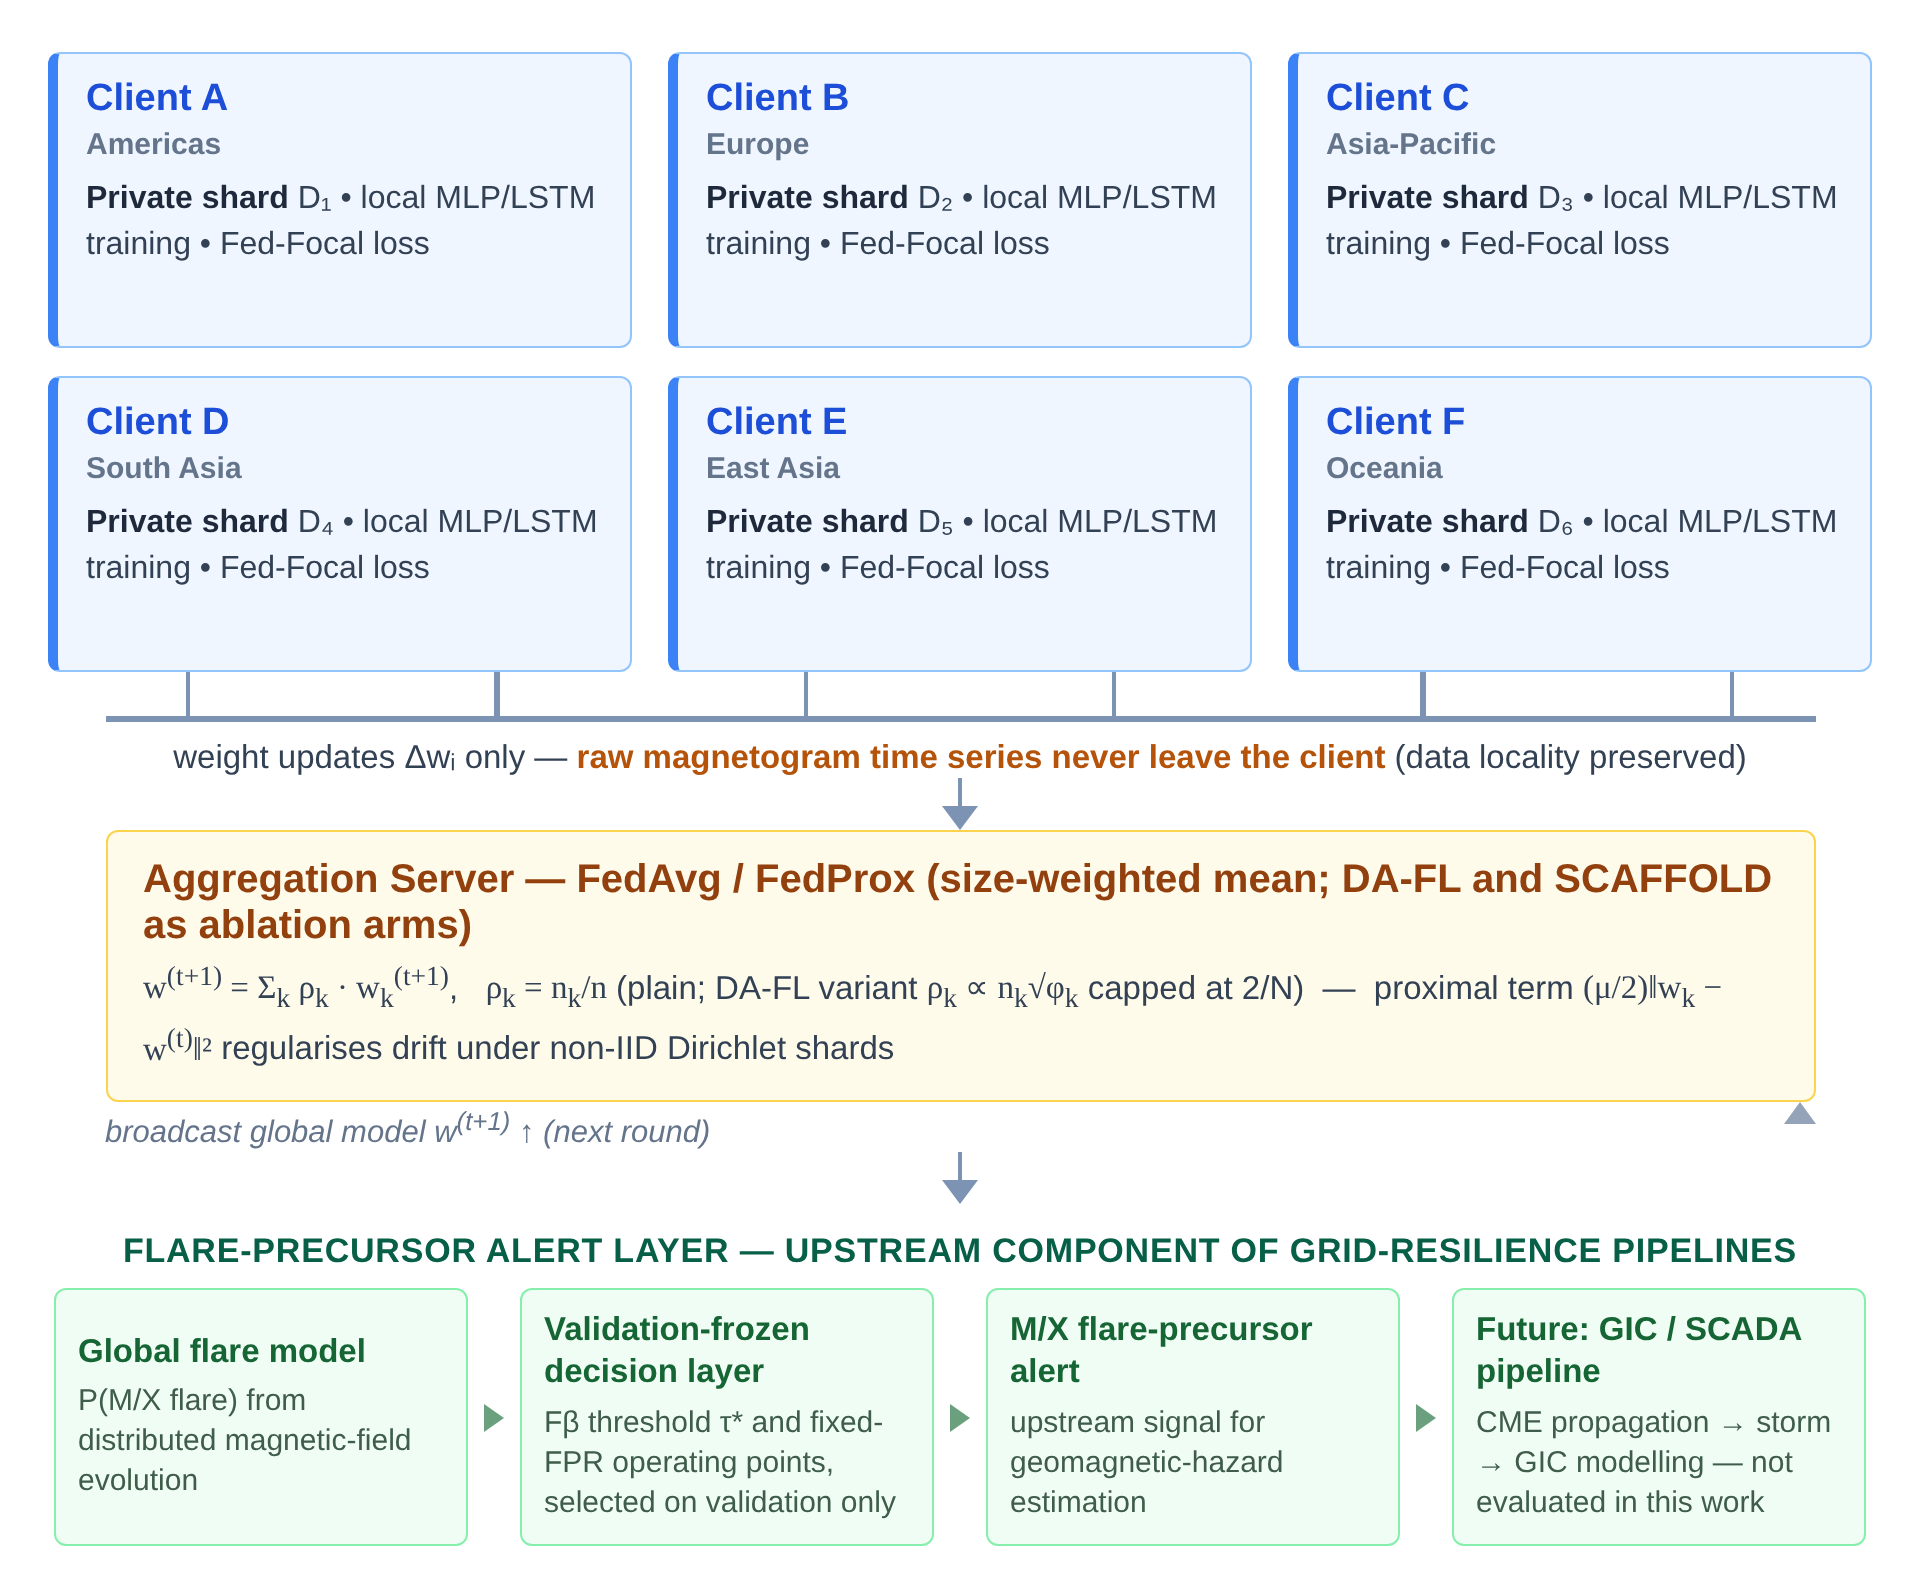
\includegraphics{figures/fig_architecture.png}
    \end{adjustbox}
    \caption{Federated benchmark-audit architecture. Six simulated
    clients (neutral labels A--F; no real institution participates)
    hold private non-IID shards of the benchmark; only model weight
    tensors $\w_k$ cross the client boundary (the figure and the
    communication-cost model describe full-weight transport; delta
    encoding is listed future compression work). The server applies
    size-weighted FedAvg/FedProx aggregation by default (the
    distribution-aware weighting $\rho_k \propto n_k\sqrt{\phi_k}$,
    capped at $2/K$, is studied as an ablation arm). The global model
    emits flare probabilities; the evaluation finds its calibration
    and frozen operating points do not survive the prevalence shift,
    so no alerting claim is made, and no downstream pipeline is
    evaluated.}
    \label{fig:arch}
\end{figure}

\subsection{Data: the SWAN-SF benchmark and its cleaned variant}

All experiments use the SWAN-SF benchmark \cite{angryk2020}
(doi:10.7910/DVN/EBCFKM), a multivariate time-series dataset of
active-region observation windows drawn from SDO/HMI vector
magnetograms, with 24 physically motivated parameters per timestep
sampled over 60-minute sliding windows and labels indicating the
occurrence of $\geq$M-class flares within the prediction horizon. The
24 parameters summarise magnetic-field complexity and include, among
others: total unsigned current helicity (TOTUSJH), total photospheric
magnetic free energy (TOTPOT), total unsigned vertical current
(TOTUSJZ), total unsigned flux (USFLUX), the sum of absolute
net-current-per-polarity (SAVNCPP), absolute net current helicity
(ABSNJZH), mean shear angle and the fraction of high-shear area
(MEANSHR, SHRGT45), the Schrijver flux-emergence proxy (R-value), and
the three components of the total Lorentz force (TOTFX, TOTFY, TOTFZ)
\cite{schrijver2007,bobra2015}.

We ingest the benchmark through its community-maintained cleaned
variant\footnote{Cleaned SWAN-SF Dataset,
\url{https://github.com/samresume/Cleaned-SWANSF-Dataset}, which
applies per-partition preprocessing: random undersampling with Tomek
links and TimeGAN-based synthetic augmentation for the training
partitions \cite{yoon2019}, LSBZM normalisation, and FPC-KNN
imputation.}, combining all five data partitions. The training
partitions are class-balanced by this preprocessing (pooled positive
rate $\bar{p} \approx 0.489$), while the untouched test partitions
retain the natural, severely imbalanced prevalence of approximately
$1.9\%$ flare windows across roughly $3.3\times10^{5}$ held-out
samples. This train--test contrast is not an artefact we introduce; it
is inherited from the benchmark's design philosophy, and it has a
consequence that shapes the entire evaluation: models trained at
$\sim$49\% prior must detect events at a $\sim$2\% prior, so absolute
probability calibration degrades and decision thresholds must be
re-optimised post hoc (Section~\ref{sec:thresholding}).

The raw-benchmark experiments of Sections~\ref{sec:res-leakfree}
and~\ref{sec:res-raw} additionally ingest the unprocessed SWAN-SF
partitions directly. The raw substrate cannot be trained on as-is:
8.87\% of its values are missing, the missingness is structured
(the Lorentz-force component TOTFZ is unobserved in 98.7\% of
training windows), and the 24 parameters span eleven orders of
magnitude. We therefore reproduce the cleaned release's two
preprocessing stages in-pipeline from their published description
(ApJS, 10.3847/1538-4365/ad7c4a) rather than inheriting their
output: a fast Pearson-correlation-based k-NN imputation (within-window
linear interpolation for partial gaps; inverse-distance-weighted
transfer of the $k{=}5$ nearest training windows' series, searched in
the space of the five most-correlated observable features, for
fully-missing series), and the LSBZM normalisation chain (robust
quantile clip, positivity shift, a log/sqrt/Box--Cox stabiliser
dispatched per feature by fitted $\lambda$, z-score, min--max), with
every parameter fitted on the training pool only and a per-feature
power-of-two pre-scaling for numerical safety. The reproduction is
verified against the released export on the audit-matched windows
(observed-position rank agreement in
Section~\ref{sec:res-raw}); where the two pipelines differ
substantively (the release re-imputes the R-value zero mass as if
missing; we preserve zeros as physical ``no flux emergence''
values), we preserve the raw semantics. The construction, the
runner, and the verification are committed as
\texttt{experiments/raw\_substrate.py},
\texttt{experiments/run\_raw\_substrate.py}, and
\texttt{experiments/run\_event\_level\_raw.py}.

\subsection{Client-side feature representation}

The framework supports two representations of the same 60-timestep
observation windows. In the MLP path used for the reported run, each
three-dimensional window $X \in \R^{60\times24}$ is reduced to a
144-dimensional statistical vector
\begin{equation}\label{eq:stats}
    \tilde{x} \;=\;
    \big[\,\mu,\;\sigma,\;\max,\;\min,\;\delta,\;s\,\big]
    \;\in\; \R^{144},
\end{equation}
where each block is applied per base feature: $\mu$ and $\sigma$ are
the temporal mean and standard deviation, $\max$ and $\min$ the window
extrema, $\delta = X_{T} - X_{1}$ the net trend, and $s$ the
least-squares slope against normalised time. This six-statistic
extraction preserves substantially more temporal information than a
temporal mean (peaks, volatility, and rate of change are precisely the
flare-relevant quantities) while remaining compatible with
weight-averaged federation and with the centralised baselines. In the
LSTM path, the raw $\R^{60\times24}$ tensor is consumed directly by a
recurrent model; this path was executed federated on the raw
substrate for all four arms plus the pooled comparator
(Section~\ref{sec:res-lstm}), with its cleaned-fold pairing remaining
future work (Section~\ref{sec:limitations}).

\subsection{Non-IID partitioning into simulated clients}

\begin{figure}[t]
    \centering
    \begin{adjustbox}{max width=0.94\textwidth, max height=0.36\textheight}
        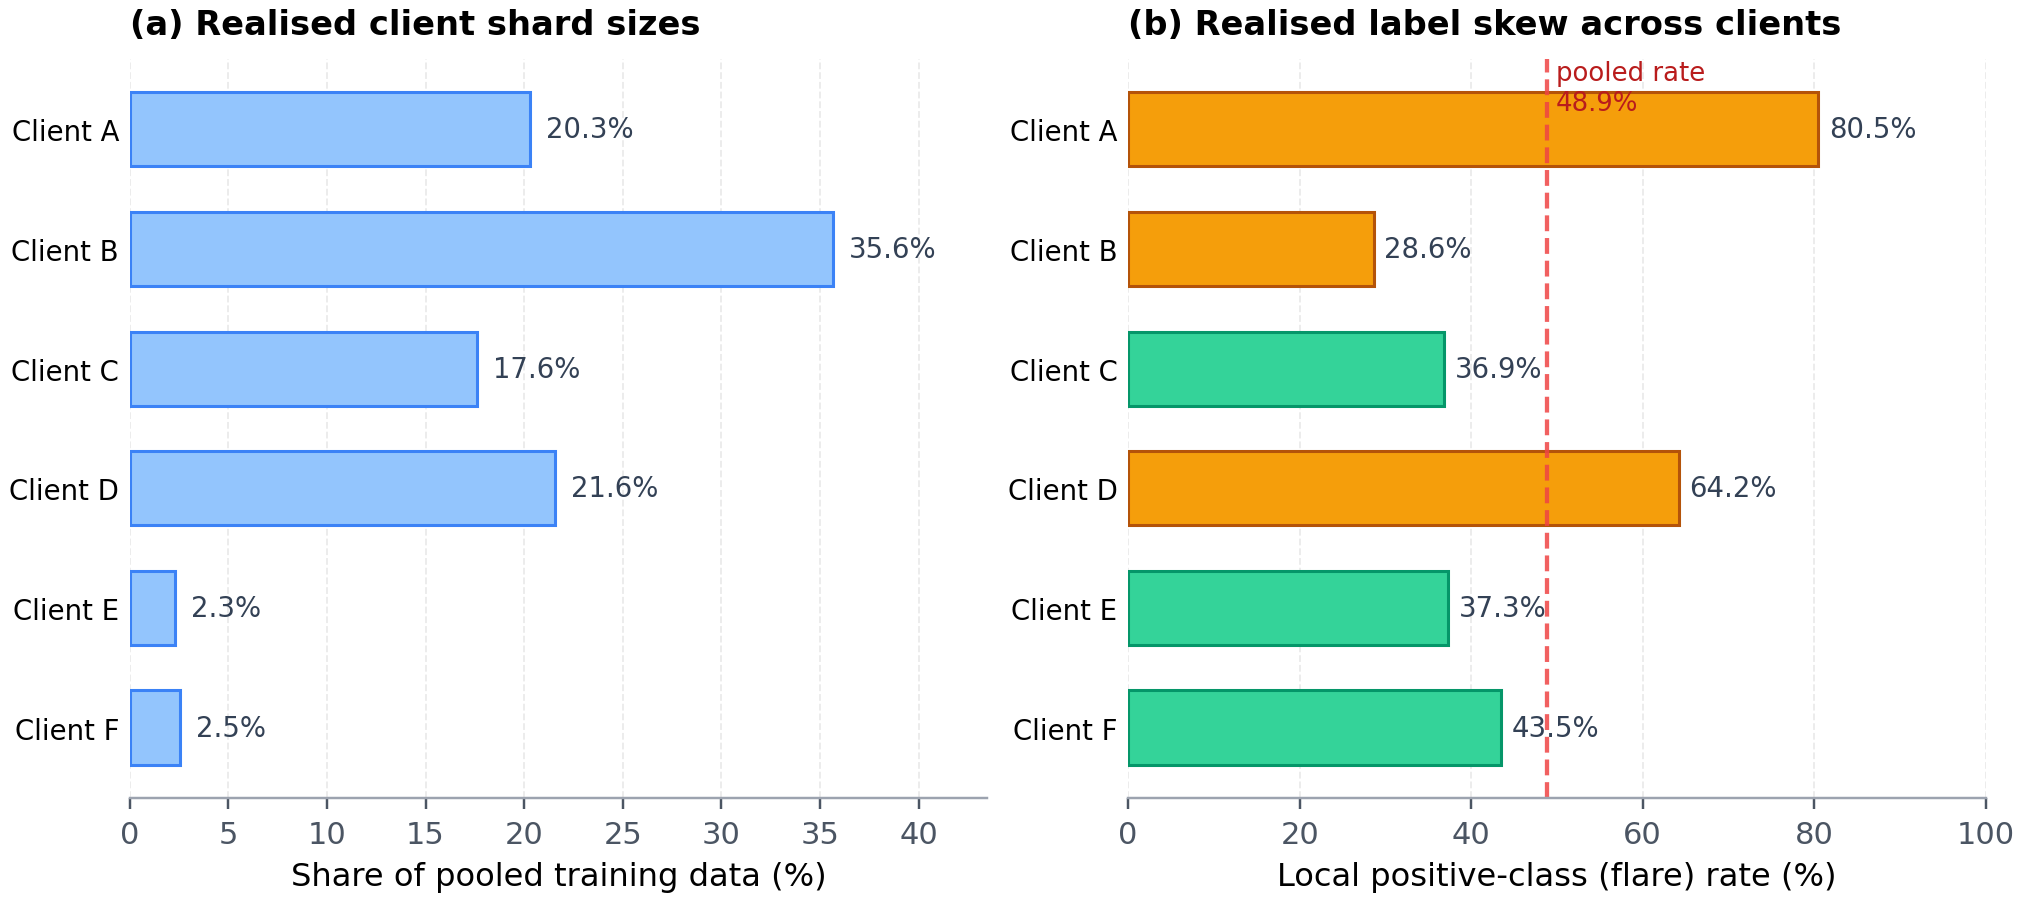
\includegraphics{figures/fig_partition.png}
    \end{adjustbox}
    \caption{Non-IID partitioning of the pooled, class-balanced
    training data into six simulated clients by label-aware Dirichlet
    sampling (concentration $\alpha = 1.0$, RNG seed 42,
    Section~\ref{sec:method}); proportions are read directly from the
    frozen run's cached client assignment. (a)~Realised relative shard
    sizes. (b)~Realised local flare rates against the pooled rate of
    48.9\%: label skew spans 28.6\%--80.5\%, emulating the label
    heterogeneity a federation would face if the shards sampled very
    different active-region populations (no real institution or
    region participates).}
    \label{fig:partition}
\end{figure}

To emulate label heterogeneity, the pooled training set is
partitioned by label-aware Dirichlet sampling: for each class $c$, a
proportion vector is drawn from
$\mathrm{Dirichlet}(\alpha,\dots,\alpha) \in \R^{K}$ and each client
receives the corresponding fraction of that class. The concentration
$\alpha$ controls heterogeneity strength---small $\alpha$ produces
near-exclusive class ownership; large $\alpha$ approaches IID.
Figure~\ref{fig:partition} shows the deterministic realisation
used by every experiment in this paper ($\alpha=1.0$, seed 42) on the
class-balanced pool: realised local flare rates span 28.6\% to
80.5\% and shard sizes range from 2.3\% to 35.6\% of the pool. This
is a deliberately hostile federation: some clients are flare-rich and
tiny, others flare-poor and large, mirroring the real asymmetry a
cross-silo federation faces when some participants' archives dominate
the pooled corpus and others sample much smaller populations. The
concentration $\alpha=1.0$
itself is the outcome of a documented tuning process
(Appendix~\ref{sec:appendix}): early experiments at $\alpha \le 0.5$
produced pathological partitions (0.3\%--99.8\% local flare rates,
re-measured under the frozen seed) under
which no aggregation scheme remained stable.

\subsection{Client models}

The primary federated architecture is a four-layer multilayer
perceptron, $\mathrm{SolarMLP}: \R^{144} \to \R$, with hidden widths
$144 \to 128 \to 64 \to 32 \to 1$, batch normalisation, ReLU
activations, and dropout $0.3$ after each hidden layer; the single
output is a raw logit consumed by the sigmoid-based losses below. MLPs
are natural federation citizens because every parameter is a
numerically meaningful averageable tensor. The released framework also
implements $\mathrm{SolarLSTM}$, a (optionally bidirectional) two-layer
LSTM with hidden size 128, Xavier/orthogonal initialisation, and a
forget-gate bias of one for long-horizon memory, followed by a
two-layer classification head \cite{hochreiter1997,hassani2025}. Local
training uses AdamW \cite{loshchilov2019} with cosine-annealing warm
restarts and gradient-norm clipping at $5.0$. We deliberately keep
XGBoost out of the federation loop: gradient-boosted tree ensembles
store discrete structure that cannot be meaningfully averaged, so the
centralised XGBoost serves as the pooled upper bound rather than a
federated participant.

\subsection{Federation algorithms and aggregation}

Three cross-silo algorithms are implemented. \textbf{FedAvg}
\cite{mcmahan2017}: each round, every client initialises from the
broadcast global model, performs $E=10$ local epochs, and the server
averages the returned weights. \textbf{FedProx} \cite{li2020}: identical
to FedAvg except each client's local objective is regularised by the
proximal term of Eq.~\eqref{eq:fedprox} with
$\mu = 0.01$, penalising drift from the global model---the mechanism
we hypothesise is decisive under the label skew of
Figure~\ref{fig:partition}. \textbf{SCAFFOLD} \cite{karimireddy2020}:
variance reduction via client and server control variates; it is
implemented with the SGD-based update required for exactness of the
control-variate correction (AdamW's adaptive steps would invalidate
the correction terms). Five implementation details depart from the
reference algorithm and are disclosed for exactness: (i)\ the
control-variate correction is damped, rescaled to 10\% of each
parameter's gradient norm (the undamped correction destabilised
training on this benchmark's loss scale); (ii)\ gradients are clipped
to max-norm 1.0; (iii)\ the shipped optimiser is SGD with momentum
$0.9$ at a learning rate of $2.5\times10^{-4}$ --- half the global
rate --- a departure of a milder class, since momentum biases the
average-gradient estimate that the control-variate update divides by
(disclosed at v4.5); (iv)\ the client control-variate update is
\emph{sign-inverted} relative to Eq.~11 of the reference algorithm:
the repository computes
$c_i^{+} = c_i - c + (y_i^{+} - y_i)/(\eta K)$ --- the negative of
the client's average local gradient --- where Karimireddy et
al.\ specify $c_i^{+} = c_i - c + (y_i - y_i^{+})/(\eta K)$; a
scalar one-client simulation of the code path confirms the inversion
exactly (the update evaluates to $-1.0000$ times the average local
gradient), and the wrongly-signed variate estimates push the
correction term $c - c_i$ the wrong way over rounds --- the damping
of item~(i) and the variate clamping bound the damage, which is why
the arm still trains (found by Dossier R-FS9-R6, disclosed at
v4.6); and (v)\ the arm is trained \emph{cold}: on every path that
produced a published operating point --- the raw-substrate MLP and
LSTM arms --- the model starts from a fresh random initialisation at
half the global learning rate, not from a converged FedAvg model
(the FedAvg-initialised warm start claimed at v3.9--v4.5 exists only
on the cleaned-fold path, where the arm is never executed; the v4.6
correction follows the call sites and the queue log, whose
validation F1 is pinned at zero through round thirty --- the
cold-start signature). A cold start at half the global rate is a
\emph{harder} protocol than the FedAvg-initialised refinement
previously claimed, so the arm's published trajectory should be read
as a from-scratch run. One further arm-level asymmetry is disclosed
at v4.5: the published SCAFFOLD operating points were trained before
the imbalance factor's global-prevalence fix (founding-audit finding
B13) was extended to the SCAFFOLD local path, so that arm's focal
weight used the hardcoded cleaned-substrate prevalence $0.4887$ as
$\bar{p}$ rather than the computed global rate the FedAvg and
FedProx arms use; on the roughly two-percent-positive raw substrate
the imbalance factor saturates at its clamp either way, which bounds
the effect. The call site is aligned at v4.5, so all three federated
arms share one loss definition in the released code, and the same
alignment is extended at v4.6 to the centralised comparators (the
pooled MLP, the budget-matched re-run, and the pooled LSTM), whose
published operating points likewise predate the plumbing and trained
under the same hardcoded-prevalence fallback --- an asymmetry of
exactly the bounded class disclosed above for the SCAFFOLD arm,
disclosed here for the central side as well (Dossier R-FS9-R6,
R8-5). Because every
published SCAFFOLD operating point was produced by this
implementation, the arm's comparisons against its siblings measure
\emph{this implementation}, not the reference algorithm: the
raw-substrate cells of Sections~\ref{sec:res-raw}
and~\ref{sec:res-lstm} --- the MLP instance's hardest-failure mode
and the sequence instance's highest event-level detection --- are
implementation-case evidence for a sign-inverted, cold-start,
damped SCAFFOLD, and a sign-corrected, warm-started vanilla
replication under the frozen protocol is queued owner-GPU future
work whose outcome may differ. The arm was held out of the
cleaned-substrate headline configuration for stability reasons and
is not run on the cleaned fold, but it is executed on the raw
substrate for both encoders, where its MLP instance is the hardest
failure and its sequence instance completes the four-arm federation
matrix (Sections~\ref{sec:res-raw} and~\ref{sec:res-lstm}).

Aggregation is \emph{plain size-weighted averaging} in the frozen
headline configuration ($\rho_k = n_k/n$, the vanilla FedAvg
choice); distribution-aware weighting (DA-FL), in which the server
weights client $k$'s update by
\begin{equation}\label{eq:dafl}
    \rho_k \;\propto\; n_k \sqrt{\phi_k},
    \qquad
    \phi_k = \frac{p_k}{\bar{p}},
    \qquad
    \rho_k \le \frac{2}{K},
\end{equation}
with $p_k$ the client's local positive rate and $\bar{p}$ the pooled
rate known to the server, is implemented as an \emph{ablation arm}
(Section~\ref{sec:res-ablation}). The square-root damping and the
$2/K$ cap prevent a flare-rich client from dominating the global
model while still up-weighting the clients most likely to contain
decision-relevant minority samples. Class-rate metadata is
deliberately much coarser than raw data and is treated as shareable
under the data-locality constraint.

\subsection{Fed-Focal loss and local rebalancing}

Each client trains with a server-aware focal loss in the Fed-Focal
family \cite{sarkar2020},
\begin{equation}\label{eq:focal}
    \ell_{\mathrm{fedfocal}}
    \;=\; -\,\alpha_t\,\bigl(1 - p_t\bigr)^{\gamma}
    \log\bigl(p_t\bigr),
    \qquad \gamma = 2.0,
\end{equation}
where $p_t$ is the model's probability of the correct class and
$\alpha_t$ interpolates between $\alpha$ and $1-\alpha$ by label. The
positive-class weight $\alpha$ is computed per client as the base value
$0.25$ \cite{lin2017} scaled by a square-root-damped imbalance factor
$\min\!\big(\sqrt{\bar{p}/p_k},\,1.5\big)$ --- with the client rate
floored at $\max(p_k, 0.01)$ so a flare-free client cannot divide by
zero --- and a mild round-progress factor in $[0.9,\,1.1]$
(linear in round progress; the $[0.7,\,1.3]$ range of an earlier
revision inflated $\alpha$ past its clamp), then clamped to
$(0.05, 0.25)$. Both constants are v4.6 disclosures completing the
loss definition (Dossier R-FS9-R6 R8-12). This clamping is a hard-won
design decision: unclamped adaptive weighting (earlier versions allowed
$\alpha$ up to $0.95$) systematically inflated positive-class weight on
flare-poor clients, producing degenerate always-flare classifiers with
recall $\approx 1.0$ and precision $\approx 0.03$
(Appendix~\ref{sec:appendix}). NaN-safe clamping of $p_t$ and of the
loss itself guards the pipeline against logit explosions in early
rounds. The framework additionally supports per-client SMOTE
oversampling \cite{chawla2002} and mixup \cite{zhang2018}; both are
\emph{disabled} in the frozen configuration because the cleaned
benchmark's training partitions arrive pre-balanced (48.9\% positive),
which renders SMOTE inert---the configured oversampling ratio produces
zero synthetic samples. The balancing question is therefore
inapplicable to this benchmark variant, and we report it as a null
result rather than a contribution (Section~\ref{sec:res-ablation});
on the raw substrate, where natural prevalence gives it work to do,
the per-client SMOTE ablation has since been executed and is
likewise a clean negative (Section~\ref{sec:res-lstmrep}).

\subsection{Threshold protocol for safety-critical recall}
\label{sec:thresholding}

Because federated training operates on rebalanced local data while
deployment operates at the natural $1.9\%$ prior, the emitted
probabilities are deliberately miscalibrated, and a fixed $0.5$
threshold is meaningless. The frozen protocol therefore performs all
selection on validation data, in two stages. First, the decision
threshold is selected by sweeping $\tau$ over $[0.05, 0.95]$ in steps
of $0.005$ and choosing, per model, the $\tau^\ast$ that maximises
$\Fbeta$ with $\beta=2$ (Eq.~\eqref{eq:fbeta}) on the validation set;
$\tau^\ast$ is then frozen and applied to the test set exactly once.
All reported precision, recall, F1, and accuracy figures are taken at
each model's frozen threshold. Second---because balanced-prevalence
validation turns out not to support threshold transfer at all
(Section~\ref{sec:res-calib})---the framework additionally freezes
\emph{fixed-FPR operating points}: for each target false-positive
budget $f \in \{0.5\%, 1\%, 2\%, 5\%\}$, the threshold is set to the
$(1-f)$-quantile of \emph{validation negative scores}, a quantity that
uses no test information whatsoever; the realised test behaviour at
each frozen threshold (achieved FPR, recall, precision, alert rate) is
reported in the same single test pass. The negative-quantile rule is
numerically validated in the released test suite, and the
raw-substrate retraining of Section~\ref{sec:res-raw} supplies the
natural-prevalence validation split that is the ideal substrate for
this protocol.
ROC-AUC and PR-AUC, being threshold-free, are reported independently.

\subsection{Threat model and security posture}
\label{sec:threatmodel}

The verified property of this framework is data locality (raw data
never leaves the client), not end-to-end security. To make that scope
auditable, Table~\ref{tab:threat} states the threat model explicitly:
which adversaries are considered, which defences the released code
provides, and which are documented but unevaluated.

\begin{table}[t]
\centering
\caption{Threat model of the released framework. ``Mitigated in code''
means implemented and covered by the integrity test suite;
``documented'' means design guidance exists but no quantitative
evaluation has been performed on this benchmark.}
\label{tab:threat}
\small
\begin{tabularx}{\textwidth}{@{}>{\raggedright\arraybackslash}X >{\raggedright\arraybackslash}X >{\raggedright\arraybackslash}X@{}}
\toprule
\textbf{Adversary / attack} & \textbf{Defence} & \textbf{Status} \\
\midrule
Honest-but-curious aggregation server (observes all weight
updates) & Secure-aggregation module (Bonawitz-style masks;
tests verify arithmetic round-trip cancellation only --- the sketch
uses deterministic, publicly reproducible mask keys, so it confers
no cryptographic privacy as committed) & Implemented as a numerical
sketch; not wired into the training loop; accuracy overhead not
measured \\
\addlinespace[2pt]
Gradient inversion / reconstruction from the transcript
$\mathcal{T}$ \cite{zhu2019} & Secure aggregation (masks updates);
differential-privacy hooks & Documented; not evaluated \\
\addlinespace[2pt]
Membership inference against a specific client's training data &
Differential-privacy hooks (noise on client updates) & Documented;
not evaluated \\
\addlinespace[2pt]
Malicious client: model poisoning / backdoor insertion & None at
present; Byzantine-robust aggregation is a design note & Not
addressed \\
\addlinespace[2pt]
Client impersonation / spoofed updates & Transport security (TLS)
and client authentication are deployment infrastructure outside the
learning loop & Documented (deployment guidance) \\
\addlinespace[2pt]
Network interception of updates & TLS in transit & Documented
(deployment guidance) \\
\bottomrule
\end{tabularx}
\end{table}

For the benchmark study reported here---six simulated clients, public
data, no real adversaries---none of these defences is enabled, so the
reported accuracy numbers are those of the undefended pipeline. Any
cross-agency deployment would need to re-measure accuracy under secure
aggregation and differential privacy before the numbers in
Section~\ref{sec:results} could be quoted as expected operational
performance (Section~\ref{sec:limitations}).

\subsection{Interpretability layer}

To audit what the models learn, SHAP values \cite{lundberg2017} are
computed for the centralised XGBoost reference over a 500-sample test
subset with the TreeExplainer and for the federated model with DeepSHAP
(100-sample background), yielding mean absolute SHAP attributions per
feature. The statistical representation of Eq.~\eqref{eq:stats}
carries a 144-entry name contract---each feature is named
\texttt{<statistic>\_<parameter>} (e.g.\ \texttt{mean\_TOTUSJH},
\texttt{max\_R\_VALUE}), with the statistic blocks ordered $\mu$
(0--23), $\sigma$ (24--47), $\max$ (48--71), $\min$ (72--95), $\delta$
(96--119), $s$ (120--143) over the 24 base parameters---and the
improved pipeline preserves these names end-to-end, so the SHAP layer
reports physically meaningful attributions directly (the v2.x pipeline
lost the mapping and required an analytical decoding pass;
Appendix~\ref{sec:appendix}). Section~\ref{sec:results} presents the
raw ranking, its statistic-level structure, and the physical grouping
used for cross-model comparison.

% ════════════════════════════════════════════════════════════════════
% SECTION 5 — EXPERIMENTAL SETUP  (v3.1: frozen-protocol description)
% ════════════════════════════════════════════════════════════════════
\section{Experimental Setup}\label{sec:experiments}

\subsection{Frozen evaluation protocol}
\label{sec:protocol}

All experiments in this revision run under an immutable evaluation
contract, enforced in code before any training is permitted:

\begin{itemize}[leftmargin=1.4em,itemsep=1pt]
\item \textbf{Splits.} The benchmark's five training partitions
(97{,}764 windows, balanced, $48.87\%$ positive) form the training pool;
the five test partitions (331{,}185 windows, natural prevalence,
$1.88\%$ positive) are the held-out test set and are loaded exactly
once at the very end of the pipeline. A stratified validation set
(16\%, $n{=}15{,}643$) is carved from the \emph{training} pool with the
root seed (42) and is the only set used for any model selection.
\item \textbf{Selection isolation.} Hyperparameter monitoring, the
best-checkpoint rule, calibration fitting, the $F_\beta$ threshold
search, and the fixed-FPR operating-point thresholds all operate on
validation. The test set participates in no selection of any kind
(the v2.x pipeline selected thresholds directly on test; this
revision removes that violation).
\item \textbf{Leakage audit.} A runtime audit verifies
sample-disjointness of train/validation/test, disjointness and coverage
of the client shards, and flags the known limitation that
active-region identities are not available in the cleaned export, so
region-level separation across the train/validation boundary cannot be
guaranteed (Section~\ref{sec:limitations}). The pipeline refuses to
train if the audit fails.
\item \textbf{Single-pass evaluation.} Each model's frozen pipeline
(calibrator $+$ threshold) is applied to the test set once; all
reported test metrics are recomputed from those predictions (the v2.x
code reported a stale accuracy for federated models).
\item \textbf{Protocol extensions released with this revision.} The
following components are implemented, unit-tested (the integrity
battery of \texttt{tests/run\_battery.py}, whose canonical 219/219
record and log are committed at \texttt{logs/test\_battery.log} and
whose v4.3 extension adds the sweep-coverage checks of
\texttt{tests/test\_lag\_sweep\_artifact.py}), and smoke-validated. Five of them were additionally
\emph{executed} end-to-end in the independent re-execution of
Section~\ref{sec:repro} and their results are reported in
Section~\ref{sec:results}: (ii)\ the validation-frozen fixed-FPR
operating-point protocol of Section~\ref{sec:thresholding} (realised
test behaviour in Section~\ref{sec:res-calib}); (iii)\ the
untouched-holdout client evaluation mode, in which every client
reserves a fraction its models never train on, so local versus
global comparisons are clean generalisation estimates
(Section~\ref{sec:res-clients}); (iv)\ the budget-matched centralised
retraining (epoch cap raised to 500 in two early-stopping variants;
Section~\ref{sec:budget}); (vi)\ the calibration-comparison harness
(raw, prior-shift, Platt, isotonic, and temperature arms,
validation-fit and single-pass test evaluation;
Section~\ref{sec:res-calib}); and the $\alpha{=}5.0$ promotion run at
the full 50-round protocol (negative result; retained
$\alpha{=}1.0$; Section~\ref{sec:fedconfig}). The remaining
extensions are no longer blocked: (v)\ the event-level evaluation
module (detection rate, missed events, duplicate alerts, warning lead
time, alert rate per day) was unblocked by the raw-metadata audit of
Section~\ref{sec:provenance}---event keys and GOES peak times
recovered from the raw benchmark---and has been executed on the
trained models of both substrates
(Tables~\ref{tab:eventlevel} and~\ref{tab:eventlevel-raw}); and
(i)\ the region-disjoint train/validation split generator is released
and awaits a within-fold study design (the temporally-preceding fold
is already region-disjoint by construction,
Section~\ref{sec:provenance}, so its remaining use is
within-fold validation work).
\end{itemize}

\subsection{Baselines}

Four centralised references span the difficulty range of the task.
\textbf{Climatology} predicts the training prevalence for every window
---the skill floor. \textbf{Logistic regression} uses balanced class
weights and 2{,}000 maximum iterations. \textbf{Centralised MLP} is the
architecture-controlled reference: the identical SolarMLP
(29{,}377 parameters), trained on the pooled features with the same
loss family and decision layer — the optimisation itself differs as
Table~\ref{tab:budget} records (constant-rate AdamW with early
stopping versus cosine-warm-restart rounds; a v4.6 correction of the
cell that previously claimed the schedule for both sides) — and its
comparison against the federated MLP isolates the
effect of federation from the effect of architecture (the v2.x
manuscript lacked this baseline and compared federated MLPs only
against XGBoost). \textbf{XGBoost} \cite{chen2016} (300 estimators,
depth 6, learning rate 0.05, subsample 0.8) is the strongest reference
baseline; its \texttt{scale\_pos\_weight} (1.05) is now derived from
the \emph{training} prevalence rather than hand-set with knowledge of
the test imbalance. Every baseline receives the same
validation-selected calibration and threshold treatment as the
federated models, so the decision layer is uniform across all
comparisons.

\subsection{Federated configuration and protocol freeze}
\label{sec:fedconfig}

Table~\ref{tab:hyper} summarises the frozen configuration. The
headline runs use plain size-weighted FedAvg aggregation (the DA-FL
weighting of Eq.~\ref{eq:dafl} is studied as an ablation arm in
Section~\ref{sec:res-ablation}); per-client SMOTE is disabled because
the balanced benchmark renders it inert. The proximal coefficient is
$\mu=0.01$. Two facts govern the heterogeneity parameter: the headline
run and \emph{all} statistical studies (multiseed, ablations,
client-level evaluation) use the frozen-protocol Dirichlet
$\alpha=1.0$; separately, the $\mu/\alpha$ sensitivity sweep
($\mu \in \{0.001, 0.01, 0.1\}$, $\alpha \in \{0.5, 1.0, 5.0\}$,
15 rounds) selected $\alpha=5.0$, $\mu=0.01$ as the
validation-optimal configuration (validation PR-AUC 0.993; its single
test pass gave PR-AUC 0.297, consistent with the headline FedProx
result). The two values answer different questions---$\alpha=1.0$ is
the adversarially heterogeneous \emph{study regime}, $\alpha=5.0$ is
the validation-selected \emph{tuning optimum}---and we do not silently
substitute one for the other. The promotion experiment was executed
in this revision at the full 50-round frozen protocol
(\texttt{outputs/alpha5\_promotion.json}): FedProx at $\alpha=5.0$
reaches test ROC-AUC $0.955$ / PR-AUC $0.296$, statistically
indistinguishable from the $\alpha=1.0$ headline ($0.954$/$0.307$),
so the sweep optimum does not transfer to the study regime and
$\alpha=1.0$ is retained as the frozen headline configuration.
The same run isolates a severity threshold for the shipped-eval FedAvg
drift at $\alpha=1.0$: at $\alpha=5.0$ the identical FedAvg arm
completes all 50 rounds without the evaluated collapse (test ROC-AUC
$0.915$, PR-AUC $0.201$)---milder heterogeneity keeps the weights
compatible with the stale-buffer evaluation for longer, which is
consistent with (though not proof of) the mechanism dissected in
Section~\ref{sec:res-bn}. Both values, and the
provenance of each, are recorded in the run manifest.

\begin{table}[t]
\centering
\caption{Frozen configuration of the improved framework
(\texttt{improvements} branch).}
\label{tab:hyper}
\small
\begin{tabularx}{\textwidth}{@{}l >{\raggedright\arraybackslash}X l@{}}
\toprule
\textbf{Component} & \textbf{Setting} & \textbf{Notes} \\
\midrule
Federation & $K=6$ clients (all selected each round), $T=50$ rounds &
headline \\
Local optimisation & 10 local epochs, AdamW, lr $5\times10^{-4}$, wd
$10^{-4}$, cosine warm restarts, batch 512, grad-clip 5.0 & unchanged \\
FedProx & $\mu = 0.01$ & sweep-validated \\
Aggregation & plain size-weighted mean (DA-FL: ablation) & protocol hardening \\
Loss & Fed-Focal, $\gamma=2.0$, $\alpha$ clamped $(0.05,0.25)$; global
prevalence computed, not hardcoded & B13 fix \\
Local rebalancing & SMOTE off (inert: pre-balanced data) & ablation \\
Partitioning & Dirichlet $\alpha=1.0$, disjoint by construction,
seed 42 & B2 fix \\
MLP & $144\!\to\!128\!\to\!64\!\to\!32\!\to\!1$, BatchNorm, ReLU,
dropout 0.3, 29{,}377 params & \\
Checkpointing & restore best validation F1 round & B3 fix \\
Calibration & prior-shift (validation-fit; Platt/isotonic/temperature
available) & \\
Decision layer & $F_2$ threshold grid $\tau\in[0.05,0.95]$ on
\emph{validation} & B1 fix \\
Multi-seed & seeds 42--46, mean/std/CI95, Wilcoxon paired & new \\
Ablations & $2\times3\times2\times2$ grid, 20 rounds & new \\
\bottomrule
\end{tabularx}
\end{table}

\subsection{Metrics}

We report precision, recall, F1, $F_2$, ROC-AUC, PR-AUC, Brier score,
expected calibration error (ECE), and recall at fixed false-positive
budgets (0.5\%, 1\%, 2\%, 5\%). Given the $26\times$
validation-to-test prevalence shift and the threshold-transfer failure
documented in Section~\ref{sec:res-calib}, the threshold-independent
measures (ROC-AUC, PR-AUC, recall-at-FPR) carry the discrimination
claims, while the threshold-conditional measures document the decision
layer honestly. Confusion matrices are row-normalised. For the
multi-seed study we report mean $\pm$ standard deviation with
Student-$t$ 95\% confidence intervals and one-sided Wilcoxon
signed-rank paired tests.

\subsection{Optimisation budgets: centralized versus federated}
\label{sec:budget}

The centralised-MLP versus federated comparison is only interpretable
if the optimisation budgets of the two arms are stated explicitly, so
the pipeline now emits a machine-readable budget audit
(\texttt{training\_budget} in \texttt{results.json}).
Table~\ref{tab:budget} summarises it. The shipped budgets are
\emph{not} matched: the centralised reference executes at most 30
full passes over the pooled training set (with early stopping on
validation loss), whereas each federated client's shard receives
$50 \times 10 = 500$ local passes over the 50 rounds. The
budget-matched re-run was executed in this revision
(\texttt{outputs/budget\_matched.json}): the centralised MLP was
retrained on the same pooled data with the epoch cap raised to 500,
in two variants---(a)~early stopping retained, which fires at epoch
13 and reproduces the headline numbers exactly, and (b)~the FL-style
fixed-budget protocol (no early stop, best-validation-loss checkpoint
retained), which reaches test ROC-AUC $0.917$ / PR-AUC $0.219$. Two
conclusions follow. First, the confound ran \emph{against} the
federated arm: the shipped centralised reference was \emph{undertrained}
(early stopping fires long before the budget binds), and the pooled
model improves when granted the federated arm's budget. Second, the
improvement is not sufficient---at full budget parity the centralised
MLP ($0.917$/$0.219$) remains below FedProx ($0.954$/$0.307$) on the
threshold-free metrics, so the headline gap is a genuine federation
effect on this benchmark rather than a budget artifact (its $F_1$ of
$0.135$ versus FedProx's $0.042$ reflects threshold-transfer behaviour
under prior shift, not ranking skill). The architecture comparison
(identical 29{,}377-parameter MLP) remains matched by construction.
The raw-substrate LSTM arms (Section~\ref{sec:res-lstm}) inherit the
same asymmetry: the pooled SolarLSTM comparator is capped at 30
epochs with patience-5 early stopping (which did not fire: epoch 30,
validation BCE 0.039), while the federated arms receive 500 shard
passes. The FedProx-LSTM-over-central-LSTM margin ($+0.008$ ROC-AUC)
is therefore budget-caveated---the cleaned-fold parity experiment
moved the central MLP by $+0.029$ ROC-AUC, the same order---whereas
the load-bearing contrast of that section (federated LSTM versus
federated MLP under identical budget and aggregation) is
budget-matched by construction.

\begin{table}[t]
\centering
\caption{Training-budget audit of the two architecture-matched arms
(review finding: the comparison is confounded by optimisation budget;
the table makes the confound auditable).}
\label{tab:budget}
\small
\begin{tabularx}{0.94\textwidth}{@{}>{\raggedright\arraybackslash}X l l@{}}
\toprule
 & \textbf{Centralised MLP} & \textbf{Federated (FedProx)} \\
\midrule
Epochs / rounds & $\le$30 epochs & 50 rounds $\times$ 10 local epochs \\
Batch size & 256 & 512 \\
Learning rate (peak) & $5\times10^{-4}$ & $5\times10^{-4}$ \\
LR schedule & constant (no scheduler) & cosine warm restarts \\
Effective passes over own data & $\le$30 (pooled set) & 500 (per client shard) \\
Early stopping & patience 5 (validation BCE) & none (fixed rounds) \\
Checkpoint rule & best validation BCE & best validation F1 round \\
Budgets matched & \multicolumn{2}{l}{Shipped: no; matched 500-epoch re-run executed---see text} \\
\bottomrule
\end{tabularx}
\end{table}

\subsection{Compute and reproducibility}
\label{sec:repro}

The complete experimental programme of this revision (headline run,
24-cell ablation grid, 9-configuration sweep, 5-seed study,
interpretability, and communication measurements) was executed on a
2-core CPU-only container with under 4\,GB of RAM, in aggregate
approximately 2.5~hours of wall-clock time. Every experiment writes a
machine-readable results artefact (\texttt{results.json},
\texttt{ablation\_results.json}, \texttt{sweep\_results.json},
\texttt{multiseed\_results.json}, \texttt{interpretability.json},
\texttt{smote\_validity.json}) plus a run manifest embedding the code
version, seeds, configuration, and dataset manifest hash; all figures
and tables are generated from these artefacts. The pipeline supports
round-level crash recovery, and the integrity battery (partitioning
disjointness, leakage audit, calibration, evaluation protocol,
threshold-freezing arithmetic, event-level metrics, FL smoke tests,
GPU-queue artefact guards, a leakage-gate failure-path test, and an
audit-artefact recomputation test, joined at v4.3 by a
lag-definition-sweep cross-artefact test)
passes its canonical 219/219 record (\texttt{tests/run\_battery.py};
\texttt{logs/test\_battery.log}, torch-equipped) and 224/0 in the
v4.3 torch-less verification environment
(\texttt{logs/test\_battery\_v4.3.log}, 24 torch-dependent checks
skipped --- the same delta an independent torch-less re-run shows).

\paragraph{Independent re-execution from the public artefacts.}
Following an external review, the entire headline pipeline was
re-executed from scratch in a clean environment: the Cleaned SWAN-SF
release was downloaded from the dataset repository's official
distribution, all 20 partition files were verified byte-identical to
the frozen data manifest (SHA-256 match on every file ---
\texttt{data\_manifest/verify\_manifest.py}, whose committed log at
\texttt{logs/verify\_manifest.log} records the 20/20 verdict and the
manifest hash; the verification also runs as a hard gate at pipeline
start), and the frozen
protocol was run end-to-end (data load and flattening, immutable
splits, Dirichlet partition, pooled baselines, FedAvg and FedProx to
50 rounds, validation-fit calibration and thresholds, single-pass test
evaluation, figures, and SHAP attribution) on CPU only (the protocol
run of record used Python 3.12; the committed battery log header
records the v4.1 verification battery's environment --- python
3.13.5, numpy 2.2.4, torch 2.14.1+cpu --- the library versions
pinned in \texttt{requirements.txt}; the run manifest records them
per-run from v4.0 onward --- the committed manifest documents the
original v3.x execution and predates the field). Every test-set metric of every model
reproduced \emph{exactly}, to all reported significant digits: all
six models' ROC-AUC, PR-AUC, Brier, ECE, precision, recall, F1, and
accuracy match the published artefacts at three decimals, and the
FedAvg divergence signature reproduces (rounds 5--40 agree to three
decimals; the collapsed-tail values differ by up to 0.02 between the
original execution and the re-run caches, a chaotic regime the
diagnostic of Section~\ref{sec:res-bn} documents). The pipeline is
therefore bit-stable under this protocol: fixed seeds, deterministic
CPU kernels, disjoint index arithmetic, and single-precision training
make the published numbers re-derivable by anyone from the public
dataset and the released code, which is the strongest form of
reproducibility claim this study can make. The same re-execution
session ran, for the first time on real data, the calibration-arm
comparison (Table~\ref{tab:calib}), the untouched-holdout client
evaluation (Section~\ref{sec:res-clients},
\texttt{client\_holdout\_eval.json}), and the frozen-FPR operating
points now reported in Section~\ref{sec:res-calib}; the multi-seed,
sweep, and ablation studies were not re-executed and their numbers
remain the owner-side artefacts embedded in the repository.

\paragraph{Owner-GPU execution of the sequence arms.}
The raw-substrate LSTM arms of Section~\ref{sec:res-lstm} were
executed on owner-side GPU hardware (an NVIDIA RTX\,4060 Laptop
with CUDA and cuDNN), because the CPU-only protocol above would
have been impractically slow for the sequence arms---the one
experiment where GPU was a practical requirement. Two batches: the seed-42 arms (2.6\,h total: 0.08\,h
pooled comparator, 1.16\,h FedAvg-LSTM, 1.33\,h FedProx-LSTM) and,
as a second single resumable queue, the remaining programme (8.7\,h:
1.5\,h SCAFFOLD-LSTM, 3.9\,h the seed-43 replication of all four
arms, 3.2\,h the two SMOTE ablation arms). The substrate identity
is device-independent and asserted at startup on every run (label
equality with the frozen 2D split; a 144-statistic feature
cross-check that runs whenever the 2D cache is present, asserting
max$|$diff$|$ below the $5\times10^{-3}$ float16 bound --- on the
owner-GPU box only the 3D cache was shipped, so the label-equality
assertion ran there and the feature check ran in the CPU sessions),
and each run writes the same machine-readable
artefact schema as every CPU arm (\texttt{raw\_lstm\_eval},
\texttt{raw\_lstm\_scaffold}, \texttt{raw\_lstm\_seed43}, and
\texttt{raw\_lstm\_smote}, all under \texttt{outputs/}).
Each GPU batch was validated on receipt, before integration, by a
machine artefact audit (64 checks for the second batch: protocol
fingerprints, substrate identity, embedded frozen-counterpart
bit-matches, event-key reconciliation, and cross-checks against
the run logs). The residual device effect is kernel-level
nondeterminism in cuDNN recurrence and float-reduction order,
predicted within $\pm$0.001--0.005 on AUC-scale metrics and now
measured by the seed-43 replication at $\le$0.005 ROC-AUC on every
arm (Section~\ref{sec:res-lstmrep}); all other artefacts in this
paper were produced under the bit-stable CPU protocol above.

\paragraph{BatchNorm-transport diagnostic and no-BatchNorm control.}
Two CPU-only experiments extend the frozen protocol without altering
it. The diagnostic runner (\texttt{experiments/run\_bn\_diagnostic.py})
loads the shipped checkpoints, audits their BN buffer state, and
evaluates the returned artefacts and a faithfully re-run FedAvg
trajectory (validation history matches the frozen run within
$\pm$0.01 ROC-AUC at every logged round) under four BN treatments:
init buffers (the shipped path), exact per-client statistics pooled by
the law of total variance, per-batch statistics at evaluation time,
and the element-wise weighted average of the per-client running
statistics that local training produced in the round being evaluated.
Recalibration uses training shards only; validation and test are never
touched by it. The control runner
(\texttt{experiments/run\_nobn\_control.py}) replaces the three
\texttt{BatchNorm1d} layers with identity (28{,}929 parameters
vs.\ 29{,}377) and runs the identical 50-round loop for both
FedAvg and FedProx, with the shipped best-validation checkpoint rule
as the only selection mechanism; its per-round test evaluation is a
disclosed diagnostic, not a selection path. Both runners are
round-level resumable and write machine-readable artefacts
(\texttt{bn\_diagnostic.json}, \texttt{nobn\_control.json}) under
\texttt{outputs/}.

\subsection{Data-provenance audit and the leakage-free protocol}
\label{sec:provenance}

\paragraph{Raw-benchmark alignment.}
The Cleaned SWAN-SF export carries no region or event identifiers, so
the review-programme items that require them (region-disjoint
splits, event-level evaluation, natural-prevalence substrates) were
queued pending raw metadata. We obtained the raw benchmark from its
official distribution (Harvard Dataverse,
\texttt{doi:10.7910/DVN/EBCFKM}, 6.5\,GB across the five partition
archives plus the 34\,MB addenda with the GOES flare event lists) and
aligned every cleaned window to its raw instance. Each raw instance is
a 60-timestep CSV whose filename encodes the flare class, the
\emph{HARP} region identifier, and the window start/end timestamps,
and the folder (FL for M/X-flaring, NF otherwise) gives the label. The
matching key is the per-feature argmax/argmin position along the 60
timesteps---48 discrete invariants that survive any per-feature
monotone normalization and are robust to the export's imputation
noise. A window is accepted as aligned when at least 28 of 48
invariants agree (borderline cases require a mean per-feature Spearman
rank correlation of at least 0.70). On the test partitions this
verifies 98.7--100.0\% of windows with 100.00\% label agreement
(train-side label agreement is 99.71\% --- 161 disagreements, which
bound the synthetic-share estimate below) and a
median best-to-second-best margin of 31--32 invariants; the alignment
artefacts and per-window metadata tables are released with the code
(\texttt{outputs/dataset\_structure\_audit.json}; a committed test,
\texttt{tests/test\_audit\_artifact.py}, recomputes every headline
audit total from the committed per-partition tables and slim
metadata).

\paragraph{What the audit found.}
Three structural facts follow. First, the test export of partition
$p$ contains \emph{all} raw instances of $p$ (the counts match exactly
on every partition). Second, the training export of $p$ is a
RUS-Tomek-TimeGAN rebalanced \emph{subset of the same instances}: the
verified training pool contains 56{,}181 windows covering 56{,}005
unique raw instances (the 176-window difference is
duplicate-instance windows, 160 of them positive, all in partition
4), and \emph{every} unique verified train instance is also a test
instance (56{,}005/56{,}005; on the row basis, 56{,}181/56{,}181). Every
M/X-flaring test
instance---6{,}234 of 6{,}234, 100\% of the minority class---is in the
training pool. Third, 85.7--90.0\% of the training positive windows are
TimeGAN-synthetic (they have no raw counterpart; the 161 train-side
label disagreements bound this estimate), while virtually no
negative windows are synthetic. The release paper of the cleaned
dataset prescribes pairing \emph{temporally preceding} training
partitions with a later test partition; the shipped pipeline of this
study instead pooled the training exports of all five partitions and
evaluated on the test exports of the same five, pairing each test
partition with a rebalanced subset of itself. The published
in-partition numbers therefore partially measure memorised data,
most severely for the minority class. Because no region identifier
spans two partitions (verified: 0 shared HARPs), a
temporally-preceding fold is automatically instance-, region-, and
time-disjoint.

\paragraph{Leakage-free fold.}
All headline-model comparisons were re-run under the benchmark's
intended protocol: training on the training exports of partitions 1--4
(77{,}865 windows; 65{,}406 train / 12{,}459 validation after the
identical stratified carve), and a single-pass evaluation on the test
export of partition 5 (75{,}365 windows at the natural 1.31\%
prevalence). Everything else is frozen: Dirichlet $\alpha=1.0$, six
clients, 50 rounds, seed 42, Fed-Focal loss, prior-shift calibration
and validation-frozen thresholds. The runner is
\texttt{experiments/run\_partition\_disjoint.py} (round-resumable);
its artefacts are \texttt{outputs/partition\_disjoint\_eval.json} and,
for the event-level analysis, \texttt{outputs/event\_level\_p5.json}
with the per-window event keys recovered from the raw filenames and
the addenda GOES peak list (65 of 65 partition-5 flare events matched,
4 with multiple candidates). Event grouping uses the filename flare
tag for positive windows (one group per physical flare) and
region-day groups for background windows; alert de-duplication
applies a 1-hour cooldown within each group.

% ════════════════════════════════════════════════════════════════════
% SECTION 6 — RESULTS AND ANALYSIS  (v3.1: real frozen-protocol numbers)
% ════════════════════════════════════════════════════════════════════
\section{Results and Analysis}\label{sec:results}

All numbers in this section are produced by the improved pipeline
(improvements branch) under the frozen evaluation protocol of
Section~\ref{sec:experiments}: a single immutable
train/validation/test split, thresholds and calibration selected on
validation only, and the test set touched exactly once per model. Every
table and figure is generated from the machine-readable
results-json artefacts of the runs; no value is transcribed by
hand. The headline run uses 50 communication rounds, six clients, and
seed 42; Sections~\ref{sec:res-multiseed} and~\ref{sec:res-ablation}
quantify seed sensitivity and component attribution. An independent
re-execution of the headline pipeline from the public, byte-verified
dataset artefacts reproduces every test metric of every model exactly
(Section~\ref{sec:repro}); the calibration, frozen-FPR, and
client-holdout results below were produced in that re-execution
session.

\textbf{Protocol disclosure.} The data-provenance audit of
Section~\ref{sec:provenance} established that the in-partition
train/test pairing used by the shipped headline protocol shares
instances between the training pool and the test set---including
100\% of the flaring test instances. The subsections that follow the
present one therefore report \emph{in-partition} results: they remain
valid as evidence of protocol stability, seed sensitivity, component
attribution, and calibration behaviour under the frozen pipeline, but
they are not estimates of generalisation to unseen data. The
leakage-free evaluation under the benchmark's intended
temporally-preceding protocol is reported first, and the claims of
this study are tiered against it in
Section~\ref{sec:res-leakfree-discussion}.

\subsection{Leakage-free evaluation on the temporally-preceding fold}
\label{sec:res-leakfree}

Table~\ref{tab:leakfree} compares the five headline arms under the
leakage-free fold (training partitions 1--4, single-pass test on
partition 5) against the shipped in-partition numbers. Three
observations follow. First, \emph{discrimination generalises}: every
arm attains a ROC-AUC of at least 0.906 on the unseen partition, and
the task is evidently easier than the in-partition protocol suggested
(logistic regression reaches 0.978 / PR-AUC 0.455, the best PR ranking
of all arms together with XGBoost's 0.457). Second, the
centralised-versus-federated gap of the in-partition protocol
\emph{disappears}: the pooled centralised MLP of identical architecture
reaches 0.973 / 0.382 against FedProx's 0.976 / 0.308---a ROC
difference of 0.003 and a reversed PR ordering. The in-partition gap
(0.888 vs 0.954) was an artifact of the protocol pairing, not a
federation effect; the budget-parity re-run of
Section~\ref{sec:budget}, which controls optimisation budget but not
instance overlap, must be read in the same light. Third, the
FedProx-versus-FedAvg contrast partially survives: FedProx's ROC-AUC
(0.976) exceeds FedAvg's (0.906) by 0.070, but FedAvg's PR-AUC (0.370)
is \emph{higher} than FedProx's (0.308). The nuance is in the
checkpoint dynamics: plain FedAvg's validation F1 collapsed to zero by
round 40 and the protocol restored its round-35 checkpoint (validation
F1 0.915), so its leakage-free outcome depends on which round the
validation monitor happened to freeze. We no longer describe either
arm's outcome as checkpoint-independent: the BatchNorm diagnostic of
Section~\ref{sec:res-bn} shows the validation F1 monitor saturates at
the all-positive value $2p/(1+p)$ whenever the evaluated probabilities
saturate, and the checkpoint rule then acts on a saturated
signal---FedProx's apparent safety on this fold is that its evaluated
probabilities never crossed that regime, not that its artefact is
selection-invariant.

\begin{table}[t]
\centering
\caption{Leakage-free fold (train partitions 1--4, single-pass test on
partition 5, natural 1.31\% prevalence) against the shipped
in-partition numbers. Threshold-conditional calibration metrics
(Brier, ECE) use the validation-frozen prior-shift pipeline; ROC/PR
are threshold-free.}
\label{tab:leakfree}
\small
\begin{tabular}{@{}l c c c c c c c@{}}
\toprule
 & \multicolumn{2}{c}{\textbf{In-partition (shipped)}} &
 \multicolumn{5}{c}{\textbf{Leakage-free fold}} \\
\cmidrule(r){2-3} \cmidrule(l){4-8}
\textbf{Model} & ROC & PR & ROC & PR & Brier & ECE & R@2\%FPR \\
\midrule
Logistic regression & 0.824 & 0.235 & 0.978 & 0.455 & 0.375 & 0.477 & 0.695 \\
XGBoost (centralised) & 0.977 & 0.493 & 0.971 & 0.457 & 0.055 & 0.101 & 0.692 \\
Centralised MLP & 0.888 & 0.153 & 0.973 & 0.382 & 0.544 & 0.687 & 0.555 \\
FedAvg MLP & 0.575 & 0.199 & 0.906 & 0.370 & 0.127 & 0.337 & 0.652 \\
FedProx MLP & 0.954 & 0.307 & 0.976 & 0.308 & 0.271 & 0.508 & 0.631 \\
\bottomrule
\end{tabular}
\end{table}

The calibration and threshold-transfer failures documented
in-partition (Section~\ref{sec:res-calib}) persist leakage-free ---
on this fold the balanced-validation carve ($48.9\%$ prevalence,
partitions 1--4) again faces the natural-prevalence partition-5 test
($1.31\%$), the same 26-fold prior shift without the instance overlap ---
and are therefore genuine properties of the balanced-training /
natural-test interface rather than overlap artifacts: the
validation-frozen FPR operating points are violated by every arm
(e.g.\ XGBoost realises 15.3\% FPR at the frozen 2\% target; FedProx
49.4\%), and only XGBoost's posteriors remain usable (Brier 0.055,
ECE 0.101 versus 0.127--0.544 for the neural arms; FedAvg's 0.127
sits closest but is still an order of magnitude above the 0.013
climatology floor). The
prior-shift-corrected neural posteriors are not repairable by
threshold re-freezing on this fold either.

\paragraph{Standard verification metrics and baselines.}
Because the toolkit of Leka et al.~\cite{leka2019}---TSS, HSS, Brier
skill, reliability, persistence and climatology---is the standard
vocabulary of flare-forecast evaluation, it accompanies every stored
operating point of every evaluation substrate (the $F_\beta$
thresholds and frozen-FPR points of the in-partition, leakage-free
and raw-substrate 2-D arms, the ten raw-substrate LSTM cells, and
the event-level tables; 10-bin reliability is recomputed for the six
in-partition arms from the phase-cache models;
\texttt{experiments/run\_standard\_metrics.py} $\to$
\texttt{outputs/standard\_metrics.json}, strict JSON; the
artefact-derived blocks (A, C, D) are content-exact on re-execution,
block B's reliability recomputation additionally requires the
uncommitted phase-cache models, and the artefact embeds a wall-clock
\texttt{elapsed\_s} field, so file-level equality is not claimed).
Four findings matter. First, on the leakage-free fold
at each arm's frozen $F_\beta$ threshold, XGBoost attains TSS
$0.848$ / HSS $0.201$ (best frozen-FPR point $0.847$), logistic
regression TSS $0.489$ / HSS $0.025$, while the
neural arms sit at TSS $0.06$--$0.19$ / HSS $\le 0.006$: the
prevalence-free TSS ranking matches the PR-AUC ranking at the top
of the table (XGBoost, logistic regression, then the neural arms),
but HSS
prices the neural arms' false-alarm load severely at 1.31\%
prevalence. Second, the persistence baselines---computed on the true
time order within each active region, as the operational
verification culture mandates---set two floors, and neither is
decorative. Same-region previous-window persistence (label inertia)
achieves TSS $0.967$ / HSS $0.970$ on the partition-5 test with no
learned model at all: at a 24-hour label horizon on $\sim$60-minute
windows, an active region that is flaring is still flaring, and
\emph{no arm in this paper---XGBoost included---beats that floor}.
The 24-hour-lagged variant (forecast = the label of the same-region
window nearest $t-24$\,h, matched within $\pm$35 minutes) scores TSS
$0.418$ / HSS $0.434$; on TSS, XGBoost ($0.848$) and logistic
regression ($0.489$) are the only arms above it, and every
neural arm at its frozen threshold sits below it, while on HSS no
arm clears the floor at all (XGBoost's HSS is $0.201$). This is the
classic Leka-era result, and a benchmark audit is the right vehicle
for stating it plainly: at this window geometry the honest question
is not whether models beat persistence, but whether anything beats
\emph{lagged} persistence---and on this fold, at TSS, two arms do,
none at HSS. (An
earlier implementation of this baseline ordered windows by pool row,
whose within-region order is temporally scrambled---the median gap
between pool-row-adjacent windows is two days---so its stored value
measured randomly paired windows; that is precisely the class of
evaluation-protocol defect this paper exists to audit, and the
corrected ordering and both variants regenerate from the committed
artefact. A sensitivity sweep over eight candidate lag definitions
is committed alongside it
(\texttt{experiments/run\_lag\_definition\_sweep.py} $\to$
\texttt{outputs/lag\_definition\_sweep.json}): the seven point-lag
variants land at TSS $0.392$--$0.418$ with the same two arms
clearing each and none at HSS, while a lookback-flare variant
scores $0.964$---label inertia under another name, which no arm
clears---so the paper reports inertia and lagged persistence as
two distinct floors.) Third, no arm's raw Brier beats the climatology floor
(pooled-test BSS: XGBoost $-2.4$, FedAvg $-6.3$, FedProx $-13.3$;
all negative), and the 10-bin reliability tables confirm the
systematic over-confidence that the calibration analysis of
Section~\ref{sec:res-calib} dissects. Fourth, event-level detection
rates carry Wilson 95\% half-widths of $\pm$2.8--4.0 points on the
leakage-free fold and up to $\pm$11.8 points on the raw substrate
(65 events), and alert rates carry exact chi-square (Garwood)
Poisson intervals, so the between-arm event-level narrations of the
next paragraph are read against those bands.

\paragraph{Event-level evaluation.}
Table~\ref{tab:eventlevel} regroups the partition-5 test decisions
into physical flare events using the raw-benchmark event keys (65
M/X-class events; background windows grouped by region and day;
1-hour alert cooldown). All five arms detect effectively every event
(64--65 of 65) with a median first-alert lead time of 23.4\,h before
flare peak. That lead must be read for what it is: the label is
positive for \emph{every} window in the 24 hours before a flare, so a
median first alert near the horizon's edge measures the label
boundary, not precursor physics --- an honest reading is ``detection
fires early in the labelled window,'' not ``the model sees the flare
23 hours ahead.'' What separates the arms is their false-alarm
burden: XGBoost emits 1.7
false-alarm windows per day versus 11.6--12.7 for the neural arms, a
7$\times$ difference that mirrors the window-level calibration gap
and confirms that the deployability boundary on this benchmark is
calibration, not detection. After the 1-hour cooldown, roughly 70\%
of retained alerts are within-event duplicates, quantifying the
persistence behaviour an operations desk would face.

\begin{table}[t]
\centering
\caption{Event-level metrics on the leakage-free fold (65 true
M/X-class events, validation-frozen $F_2$ thresholds, 1-hour alert
cooldown). FA = false alarm.}
\label{tab:eventlevel}
\small
\begin{tabular}{@{}l c c c c@{}}
\toprule
\textbf{Model} & \textbf{Events detected} & \textbf{FA windows/day} &
\textbf{Alerts/day} & \textbf{Lead to peak (h)} \\
\midrule
Logistic regression & 65/65 (100\%) & 8.6 & 8.8 & 23.4 \\
XGBoost (centralised) & 64/65 (98.5\%) & 1.7 & 1.9 & 23.3 \\
Centralised MLP & 65/65 (100\%) & 12.7 & 12.8 & 23.4 \\
FedAvg MLP & 65/65 (100\%) & 11.6 & 11.8 & 23.4 \\
FedProx MLP & 65/65 (100\%) & 11.9 & 12.1 & 23.4 \\
\bottomrule
\end{tabular}
\end{table}

\subsection{Raw-substrate retraining: the unbalanced benchmark}
\label{sec:res-raw}

The leakage-free fold of Section~\ref{sec:res-leakfree} still trains
on the cleaned export---RUS--Tomek rebalanced, TimeGAN-augmented,
pre-normalised. The raw-benchmark retraining (re-run item~9,
executed in this revision) asks the complementary question: does anything in
the comparison survive when the frozen protocol is trained directly
on the \emph{raw} SWAN-SF partitions at their natural class
prevalence (2.05\% across training partitions 1--4), with no
rebalancing, no synthetic positives, and the two cleaning stages
reproduced in-pipeline? The raw benchmark cannot be trained on
directly: 8.87\% of its values are missing (42.3M of 476.9M; TOTFZ
is unobserved in 98.7\% of training windows) and the 24 parameters
span 11 orders of magnitude. The experiment therefore reproduces the
release's two preprocessing stages from their published description
(ApJS, 10.3847/1538-4365/ad7c4a): a \emph{fast
Pearson-correlation-based k-NN imputation} (partial gaps filled by
within-window interpolation; fully-missing series transferred from
the $k{=}5$ nearest training windows in the space of the five most
correlated observable features) and the \emph{LSBZM} normalisation
chain (robust clip, shift, log/sqrt/Box--Cox dispatched by fitted
$\lambda$, z-score, min--max), with every parameter fitted on the
training pool only. A verification against the released cleaned
export on the audit-matched partition-5 windows (100\% window match)
bounds the reproduction: at positions where the raw value was
observed and nonzero, rank agreement with the release has median
Spearman $\rho=0.898$ (min 0.842; the release is itself an exact
monotone image of the raw values, $\rho=1.000$, so the residual gap
is float16-storage tie dilution); at positions the release imputed,
agreement is method-dependent (median $\rho=0.313$), and for the
R-value flux-emergence proxy the release re-imputes the entire
zero mass (60.9\% of that column) as if it were missing, whereas
this reproduction preserves zeros as physical values. The three
substrates therefore differ in composition as well as in
preprocessing provenance, which is precisely the contrast the
experiment isolates.

Table~\ref{tab:rawsubstr} reports the six arms under the identical
frozen protocol (Dirichlet $\alpha{=}1.0$, six clients, 50 rounds,
Fed-Focal, seed 42, prior-shift calibration, validation-frozen
thresholds). The result is decisive and asymmetric.
\emph{Centralised arms are substrate-robust}: logistic regression is
unchanged to the third decimal (0.978, PR 0.448 vs 0.455), the
centralised MLP retains 0.971 ROC-AUC and its PR-AUC \emph{rises}
from 0.382 to 0.445, and XGBoost keeps 0.974 ROC-AUC while its
PR-AUC falls from 0.457 to 0.329---the synthetic TimeGAN positives
were inflating its minority-class precision, not teaching it.
\emph{Federated arms are substrate-fragile}: FedProx degrades from
0.976/0.308 to 0.930/0.149; plain FedAvg's PR-AUC collapses from
0.370 to 0.056 (its calibrated posteriors never cross the
validation-frozen threshold: test recall 0.000); and SCAFFOLD---the
one re-run item that had never been executed on any real
substrate---fails outright at 0.768/0.057 with Brier 0.137 (every
SCAFFOLD cell in this section measures the implementation's five
disclosed departures from the reference algorithm,
Section~\ref{sec:method}, and is read below as implementation-case
evidence). The
federated-versus-centralised ordering of the leakage-free fold was
still a property of the balanced training substrate; on the raw
unbalanced benchmark the focal-loss clients cannot learn the 2\%
minority class through 6-client Dirichlet heterogeneity, and the
gap between the best federated and best centralised arm widens to
0.048 ROC-AUC and $3\times$ PR-AUC.

One disclosure this section carried from v4.8, now resolved: the
three federated \emph{MLP} rows of Table~\ref{tab:rawsubstr} are
evaluated through the same untransported-BatchNorm path that
Section~\ref{sec:res-bn} indicts in-partition --- the runner
transports model \emph{parameters} only, so the returned
checkpoints carry never-updated running buffers into a
\texttt{model.eval()} evaluation. Until v4.9 the raw-substrate MLP
degradation above was therefore \emph{BN-evaluation-conditional} on
its face; the checkpoint-level diagnostic has since been executed
(Section~\ref{sec:res-rawbn}, \texttt{raw\_bn\_diagnostic.json}) and
the condition resolves \emph{against} the BN explanation: no
treatment recovers the centralised reference, pooled recalibration
actively destroys ranking, and the deficit is a property of the
flattened-feature arms under federation. The sequence arms are
outside the confound entirely (SolarLSTM carries no BatchNorm), so
the encoder-contrast reading of Section~\ref{sec:res-lstm} stands
either way.

\begin{table}[t]
\centering
\caption{Raw-substrate retraining (train raw partitions 1--4,
natural 2.05\% prevalence, FPCKNN/LSBZM reproduced in-pipeline with
train-only parameters; single-pass test on raw partition 5, natural
1.31\% prevalence; identical frozen protocol). The leakage-free
cleaned-substrate fold is reproduced for comparison; SCAFFOLD was
not run on the cleaned fold.}
\label{tab:rawsubstr}
\small
\begin{tabular}{@{}l c c c c c c@{}}
\toprule
 & \multicolumn{2}{c}{\textbf{Fold (cleaned)}} &
 \multicolumn{4}{c}{\textbf{Raw substrate}} \\
\cmidrule(r){2-3} \cmidrule(l){4-7}
\textbf{Model} & ROC & PR & ROC & PR & Brier & R@2\%FPR \\
\midrule
Logistic regression & 0.978 & 0.455 & 0.978 & 0.448 & 0.053 & 0.732 \\
XGBoost (centralised) & 0.971 & 0.457 & 0.974 & 0.329 & 0.018 & 0.587 \\
Centralised MLP & 0.973 & 0.382 & 0.971 & 0.445 & 0.010 & 0.596 \\
FedAvg MLP & 0.906 & 0.370 & 0.875 & 0.056 & 0.013 & 0.063 \\
FedProx MLP & 0.976 & 0.308 & 0.930 & 0.149 & 0.032 & 0.343 \\
SCAFFOLD MLP & --- & --- & 0.768 & 0.057 & 0.137 & 0.175 \\
\bottomrule
\end{tabular}
\end{table}

The event-level evaluation on the same substrate
(Table~\ref{tab:eventlevel-raw}) makes the collapse operational: all
65 true M/X-class events are matched to their GOES peaks exactly as
in the cleaned fold, but plain FedAvg now detects \emph{zero} of
them, FedProx detects 48 (73.8\%) at 1.3 false-alarm windows per
day, and SCAFFOLD's 83.1\% detection rate is bought at 6.4
false-alarm windows per day---roughly $20\times$ the centralised
arms' burden. The centralised arms detect 61.5--80\% of events at
0.2--0.3 false-alarm windows per day with 18--23\,h median lead
times. The sequence arms appended below the rule
(Section~\ref{sec:res-lstm}) restore partial federated detection
and are discussed there. Detection under class balance, in other
words, was the
artifact; under the benchmark's natural prevalence the deployable
models are exactly the ones that never needed federation.

\begin{table}[t]
\centering
\caption{Event-level metrics on the raw substrate (65 true M/X-class
events, validation-frozen $F_2$ thresholds, 1-hour alert cooldown;
99.86\% of test windows matched to the audit's event keys). The
sequence arms (below the rule) are evaluated by the standalone
torch-free CPU runner over the owner-GPU run's stored per-window
test probabilities and the same audit metadata; the SCAFFOLD-LSTM row
was evaluated in-runner by the same event-level machinery during
the second GPU batch. Median leads are rounded to 0.1\,h except the
SCAFFOLD-MLP cell, whose stored median (1{,}395\,min) is exactly
23.25\,h and is shown at full precision (T2 erratum, v4.8).}
\label{tab:eventlevel-raw}
\small
\begin{tabular}{@{}l c c c c@{}}
\toprule
\textbf{Model} & \textbf{Events detected} & \textbf{FA windows/day} &
\textbf{Alerts/day} & \textbf{Lead to peak (h)} \\
\midrule
Logistic regression & 51/65 (78.5\%) & 0.3 & 0.4 & 22.8 \\
XGBoost (centralised) & 40/65 (61.5\%) & 0.2 & 0.3 & 18.0 \\
Centralised MLP & 52/65 (80.0\%) & 0.3 & 0.4 & 20.5 \\
FedAvg MLP & 0/65 (0.0\%) & 0.0 & 0.0 & --- \\
FedProx MLP & 48/65 (73.8\%) & 1.3 & 1.4 & 23.0 \\
SCAFFOLD MLP & 54/65 (83.1\%) & 6.4 & 6.6 & 23.25 \\
\midrule
Centralised LSTM & 41/65 (63.1\%) & 0.3 & 0.4 & 19.3 \\
FedAvg LSTM & 35/65 (53.8\%) & 0.2 & 0.2 & 17.4 \\
FedProx LSTM & 49/65 (75.4\%) & 0.4 & 0.5 & 23.2 \\
SCAFFOLD LSTM & 55/65 (84.6\%) & 0.4 & 0.5 & 23.2 \\
\bottomrule
\end{tabular}
\end{table}

\subsection{Raw-substrate BN diagnostic: resolving the v4.8 condition}
\label{sec:res-rawbn}

The v4.8 revision shipped the runner for this diagnostic
(\texttt{experiments/run\_raw\_bn\_diagnostic.py}) and queued its
execution owner-side; it has since run (RUNLOG ask \#4), and its
artefact of record --- \texttt{outputs/raw\_bn\_diagnostic.json},
sha-pinned by the battery --- is what this subsection reads. One
structural fact precedes the numbers, disclosed at equal length in the
RUNLOG: the v3.x-era raw-substrate checkpoints were \emph{never
persisted} (that era's runner stored the 3D caches and the
sequence-arm checkpoints, not the seed-42 MLP weights), so the
same-weights counterfactual the diagnostic was designed around is
unavailable by construction. The run therefore re-evaluated a fresh
seed-42 replication: the substrate was rebuilt from the surviving 3D
cache (one additional f16 quantisation, within the $5\times10^{-3}$
series bound the cache format documents), the three arms were
retrained round-resumably under the frozen protocol, and the
diagnostic then applied its three BN treatments to those identical
weights. The replication is close at the substrate level: the pooled
baselines reproduce the published rows to $\le 2.3\times10^{-3}$
ROC-AUC (logistic regression $+1.7\times10^{-4}$, XGBoost
$+1.5\times10^{-3}$, centralised MLP $-2.3\times10^{-3}$), which
isolates the federated arms' gate deltas --- ROC-AUC $+0.023$
(FedAvg), $-0.002$ (FedProx), $-0.005$ (SCAFFOLD) --- as retrain
nondeterminism concentrated in the highest-variance arm. The gate
recorded MISMATCH on all three arms (tolerance $10^{-4}$) and exited
non-zero as designed; the record is frozen with that verdict.

\begin{table}[t]
\centering
\caption{The raw-substrate BN diagnostic
(\texttt{raw\_bn\_diagnostic.json}, v4.9): test ROC-AUC / PR-AUC of
the identical replication weights under the three BN treatments, per
federated MLP arm. A: the published init-buffer evaluation path; B:
exact per-client statistics pooled by the law of total variance
(training shards only); C: evaluation-time batch statistics. Gate
$\Delta$ is arm A's ROC-AUC delta against the published rows of
Table~\ref{tab:rawsubstr} (the disclosed MISMATCH; FedAvg carries
the replication's retrain variance).}
\label{tab:rawbndiag}
\small
\begin{tabular}{@{}l c c c c@{}}
\toprule
\textbf{Arm} & \textbf{A: init buffers} & \textbf{B: pooled} &
\textbf{C: batch stats} & \textbf{Gate $\Delta$} \\
\midrule
FedAvg   & 0.898 / 0.070 & 0.501 / 0.015 & 0.915 / 0.227 & $+0.023$ \\
FedProx  & 0.928 / 0.149 & 0.500 / 0.013 & 0.920 / 0.251 & $-0.002$ \\
SCAFFOLD & 0.763 / 0.053 & 0.500 / 0.013 & 0.757 / 0.069 & $-0.005$ \\
\bottomrule
\end{tabular}
\end{table}

Table~\ref{tab:rawbndiag} yields the reading, and it is the opposite
of the in-partition pattern of Section~\ref{sec:res-bn}. First,
\emph{the raw-substrate MLP deficit is not a manufactured collapse}:
arm A --- the very path the in-partition diagnostic indicts --- holds
0.763--0.928 ROC-AUC on every arm here, where the in-partition
collapse scored 0.575, and no treatment approaches the centralised
reference (0.969 on the same replication): the residual deficit,
roughly 0.04--0.21 ROC-AUC depending on arm and treatment, is a
property of the flattened-feature arms under federation, not of the
buffer-transport protocol. Second, \emph{pooled recalibration is
actively destructive here}: arm B collapses every arm to chance
(0.500--0.501), whereas in-partition the same oracle \emph{recovered}
FedAvg from 0.575 to 0.893 --- pooling exact per-client statistics
across 6 heterogeneous raw-prevalence clients inflates variance past
the point where any single pooled normalisation ranks the test
distribution, so the in-partition ``optimistic recalibration rescue''
does not transfer to the natural-prevalence substrate at all. Third,
evaluation-time batch statistics (arm C) move ROC-AUC by at most
0.017 while sharpening the positive score scale (PR-AUC
0.070$\to$0.227 for FedAvg, 0.149$\to$0.251 for FedProx): a
calibration instrument, not a rescue. The diagnostic's event-level
layer also records the operating-point pathology the A-path
thresholds inherit --- the replication's checkpoint rule returned
best-val-F1 states of 0.0 for FedAvg and FedProx, FedAvg's val-frozen
threshold sat at the 0.05 floor, and the arm detects 0 of 65 events
under A while arm C, the only treatment with a usable validation
operating point, detects 38 (58.5\%) at 0.28 false-alarm windows per
day (FedProx: 62 at 2.8 under A, 50 at 0.43 under C). The v4.8
condition is therefore closed with a precise scope: untransported BN
statistics can manufacture collapse --- in-partition proved that ---
but the raw-substrate federated MLP degradation is not that
phenomenon, and the sequence arms (no BatchNorm) were never exposed
to it.

\subsection{The sequence encoder rescues the federated arms}
\label{sec:res-lstm}

The raw-substrate collapse of Table~\ref{tab:rawsubstr} is a
statement about the flattened-feature MLP arms, and the second half of
re-run item~8 asks exactly that question: does the same frozen
protocol survive natural prevalence when the federated encoder is
sequential? The LSTM arms were executed on owner-side GPU hardware
(RTX\,4060 Laptop, cuDNN; 2.6\,h total wall-clock for both
federated arms plus the pooled comparator, against a CPU-only
sandbox run that would have been impractically slow---the one experiment where a GPU was a
practical requirement rather than a convenience). The
substrate is identical by construction: the runner rebuilds the 3D
series from the same cached stage-A/B arrays, asserts label equality
with the frozen 2D split at startup, runs the 144-statistic feature
cross-check whenever the 2D cache is present (max$|$diff$|$ bounded
by $5\times10^{-3}$ at float16 storage; on the owner-GPU box the
label-equality assertion alone ran, the 2D cache being absent
there), and reuses the
identical seed-42 Dirichlet shards, so the only degrees of freedom
are the encoder and the device. The SolarLSTM (219,265 parameters,
consuming the raw $60\times24$ series directly) is trained under the
same Fed-Focal loss, prior-shift calibration, and validation-frozen
threshold machinery as every other arm. The one arm still unexecuted
in the second owner-GPU batch---SCAFFOLD-LSTM, whose MLP instance is the hardest failure
on this substrate---was subsequently run in a second owner-GPU batch
together with the seed-43 replication and the SMOTE ablation
reported below, under the client-side fixed-step SGD that the
control-variate arithmetic requires (the AdamW invalidation of
Section~\ref{sec:discussion} is avoided by construction in the
federated implementation).

Table~\ref{tab:lstmraw} reports the outcome alongside each arm's
frozen MLP counterpart, and the asymmetry of
Section~\ref{sec:res-raw} inverts. Centrally, the LSTM is the
\emph{weaker} architecture: 0.962/0.314 against the central MLP's
0.971/0.445 on the same windows. Federated, the ordering reverses.
FedAvg-LSTM holds 0.958/0.305 where the FedAvg MLP fell to
0.875/0.056---a $+0.083$ ROC-AUC and $+0.249$ PR-AUC swing from the
encoder alone, under identical shards, budgets, and aggregation.
FedProx-LSTM reaches 0.970/0.404: above its own pooled centralised
comparator ($+0.008$ ROC, $+0.090$ PR) and above XGBoost's raw
PR-AUC (0.329). SCAFFOLD-LSTM lands at 0.970/0.294 against its MLP
counterpart's 0.768/0.057---the largest single encoder swing on
this substrate ($+0.202$ ROC-AUC, $+0.238$ PR-AUC): the hardest
failure of the flattened-feature matrix is fully recovered by the
sequence encoder under the identical protocol, completing the
four-arm federation matrix on this benchmark. The two contrasts isolate what happened. Between
federated arms of identical budget and aggregation, the sequence
encoder removes the natural-prevalence collapse the MLP suffers; the
load-bearing comparison is budget-matched by construction. Between
the pooled and federated instances of the same sequence encoder,
federation costs nothing (FedAvg) or appears to help (FedProx)---but
the latter margin carries a budget caveat, since the central
comparator is capped at 30 epochs while the federated arms receive
500 shard passes, and the cleaned-fold parity experiment moved the
central MLP by $+0.029$ ROC-AUC under exactly that correction
(Section~\ref{sec:budget}).

What does not change is at least as important. No federated arm
exceeds the best centralised baseline on either rank metric
(FedProx-LSTM sits 0.008/0.044 below logistic regression). The
frozen-$F_\beta$ thresholds transfer badly for three of the four
arms: validation $F_2$ values of 0.727/0.765/0.593 degrade to test
values of 0.405/0.309/0.499 under the $1.6\times$ validation-to-test
prevalence shift, while SCAFFOLD-LSTM is the exception---its
validation $F_2$ of 0.530 lands at 0.528 on test at a recall-heavy
operating point (test recall 0.737)---and the frozen-FPR operating
points still realise their targets within band, reproducing
(including the same conservative drift at the 0.5\% target) the
behaviour already documented for the MLP arms. Calibration remains
the deployability boundary: all three federated sequence arms beat
the raw-substrate climatology floor of 0.013 (FedAvg 0.0112,
FedProx 0.0106, SCAFFOLD 0.0120, against every federated MLP arm at
or above it, 0.013--0.137), but FedProx-LSTM's ECE of 0.020 is four
times the central LSTM's 0.005, SCAFFOLD-LSTM carries the worst
sequence-encoder calibration (0.035), and the centralised MLP's
Brier of 0.010 remains the best of all ten arms executed on this
substrate. Finally, the FedProx-over-FedAvg stabilisation now
appears on every substrate--encoder combination executed
(in-partition MLP 0.954 vs 0.575; cleaned fold 0.976 vs 0.906; raw
MLP 0.930 vs 0.875; raw LSTM 0.970 vs
0.958, replicated at seed 43 as 0.965 vs 0.961)---the most
replicated single finding of this study. The
event-level pass (bottom block of Table~\ref{tab:eventlevel-raw})
was executed offline, on CPU, from the GPU run's stored per-window
test probabilities over the same audit metadata---no retraining,
65/65 GOES peaks matched. Where plain FedAvg-MLP detects \emph{zero}
of the 65 events, FedAvg-LSTM detects 35 (53.8\%) at 0.2
false-alarm windows per day: the encoder rescue survives the
validation-frozen thresholds and the cooldown machinery, not just
the ranking metrics. FedProx-LSTM is the standout: 49/65 (75.4\%)
detection at 0.4 false-alarm windows per day, exceeding
FedProx-MLP's raw detection while cutting its false-alarm burden
$3.5\times$ (1.3), with a 23.2\,h median first-alert lead to flare
peak---the joint-longest on this substrate, and (like every arm's
lead at this label geometry) a label-boundary quantity rather than a
usable warning time (Table~\ref{tab:eventlevel}). SCAFFOLD-LSTM---measuring,
like every SCAFFOLD cell, the sign-inverted, cold-start variant of
the five-departure list in Section~\ref{sec:method}, not the
reference algorithm---evaluated in-runner by the same machinery,
supplies the sharpest
event-level datum of the batch: 55/65 (84.6\%) detection at 0.41
false-alarm windows per day and a 23.2\,h median lead---its MLP
twin's 83.1\% detection rate at one-fifteenth its false-alarm
burden, and nominally above the centralised detection frontier
(logistic regression 78.5\%, centralised MLP 80.0\%, both at
0.2--0.3 per day). The crossing is an operating-point purchase
rather than a ranking win---it is bought with $1.5$--$2\times$ the
centralised arms' alarm budget, the window-level ranking still
sits below logistic regression by 0.008/0.154, and the arm carries
the worst sequence-encoder calibration (ECE 0.035)---so the
data-locality conclusion of Section~\ref{sec:res-raw} survives at
event level with this one priced exception.

\begin{table}[t]
\centering
\caption{Raw-substrate LSTM arms (frozen protocol, identical
substrate, shards, and evaluation as Table~\ref{tab:rawsubstr};
owner-GPU execution, seed 42) with each arm's frozen MLP counterpart
repeated from Table~\ref{tab:rawsubstr} for the
architecture-versus-federation contrast. Brier and ECE on the
calibrated test probabilities at natural 1.31\% prevalence. The
seed-43 replication and per-client SMOTE ablation of the same arms
are reported in Table~\ref{tab:lstmrep}.}
\label{tab:lstmraw}
\small
\begin{tabular}{@{}l cc cc c c c@{}}
\toprule
 & \multicolumn{2}{c}{\textbf{LSTM arm}} &
 \multicolumn{2}{c}{\textbf{MLP counterpart}} & & & \\
\cmidrule(r){2-3} \cmidrule(l){4-5}
\textbf{Model} & ROC & PR & ROC & PR & Brier & ECE & R@2\%FPR \\
\midrule
Centralised & 0.962 & 0.314 & 0.971 & 0.445 & 0.0111 & 0.005 & 0.481 \\
FedAvg & 0.958 & 0.305 & 0.875 & 0.056 & 0.0112 & 0.007 & 0.431 \\
FedProx & 0.970 & 0.404 & 0.930 & 0.149 & 0.0106 & 0.020 & 0.525 \\
SCAFFOLD & 0.970 & 0.294 & 0.768 & 0.057 & 0.0120 & 0.035 & 0.521 \\
\bottomrule
\end{tabular}
\end{table}

\subsection{Seed replication and the natural-prevalence SMOTE
ablation}
\label{sec:res-lstmrep}

The sequence arms executed at a single seed on a single
device, and the replication caveat that followed them is discharged
by the second owner-GPU batch: all four arms re-executed at seed 43
(model initialisation and the Dirichlet shard draw reseeded, the
frozen validation carve kept identical). The ranking structure
replicates (Table~\ref{tab:lstmrep}, middle columns)---the seed-42
FedProx/SCAFFOLD statistical tie (0.970 each) resolving into
SCAFFOLD's narrow lead at seed 43.
ROC-AUC moves by at most 0.005 on any arm (FedAvg
0.958$\to$0.961, FedProx 0.970$\to$0.965, SCAFFOLD
0.970$\to$0.968, central 0.962$\to$0.962)---inside the device and
kernel jitter band predicted in Section~\ref{sec:repro}---and
every qualitative finding survives: no arm collapses, FedProx
stays above FedAvg on both rank metrics, SCAFFOLD stays
competitive, and no federated arm approaches the centralised
ranking frontier. PR-AUC, as expected at 1.3\% prevalence, moves
more (FedAvg 0.305$\to$0.271, central 0.314$\to$0.357, SCAFFOLD
0.294$\to$0.368, FedProx 0.404$\to$0.381) without overturning any
load-bearing ordering. Event-level detection moves within a
seven-point band at comparable false-alarm rates (FedAvg
35$\to$36, central 41$\to$43, FedProx 49$\to$45, SCAFFOLD
55$\to$50 of 65). The sequence-encoder rescue is not an artefact
of one seed.

\begin{table}[t]
\centering
\caption{Seed-43 replication and per-client SMOTE ablation of the
raw-substrate sequence arms (window-level test metrics; protocol,
substrate, and evaluation identical to
Table~\ref{tab:lstmraw}). Seed 43 reseeds model initialisation and
the Dirichlet shard draw; the frozen validation carve is unchanged.
SMOTE oversamples each client's minority class to a 0.25
minority-to-majority ratio (seed 42, flattening the $60\times24$
series and reshaping).}
\label{tab:lstmrep}
\small
\begin{tabular}{@{}l cc cc cc@{}}
\toprule
 & \multicolumn{2}{c}{\textbf{Seed 42}} &
 \multicolumn{2}{c}{\textbf{Seed 43}} &
 \multicolumn{2}{c}{\textbf{Seed 42 + SMOTE}} \\
\cmidrule(r){2-3} \cmidrule(r){4-5} \cmidrule(l){6-7}
\textbf{Model} & ROC & PR & ROC & PR & ROC & PR \\
\midrule
Centralised & 0.962 & 0.314 & 0.962 & 0.357 & --- & --- \\
FedAvg & 0.958 & 0.305 & 0.961 & 0.271 & 0.961 & 0.307 \\
FedProx & 0.970 & 0.404 & 0.965 & 0.381 & 0.946 & 0.288 \\
SCAFFOLD & 0.970 & 0.294 & 0.968 & 0.368 & --- & --- \\
\bottomrule
\end{tabular}
\end{table}

The complementary ablation asks whether class rebalancing can
substitute for the encoder. Per-client SMOTE, oversampling each
shard's minority to a 0.25 minority-to-majority ratio on the
flattened $60\times24$ series, was run for the two production
federated arms at seed 42 (Table~\ref{tab:lstmrep}, right columns).
FedAvg is unchanged at window level (0.961/0.307 against 0.958/0.305
natural, with event detection even edging up, 35$\to$40 of 65);
FedProx is actively degraded:
0.946/0.288 against 0.970/0.404, a $-0.116$ PR-AUC loss, with
event detection falling 49$\to$37 of 65. The result completes the
cleaned-fold SMOTE null (Section~\ref{sec:res-ablation}: inert
there because the substrate was pre-balanced) at natural
prevalence, where it has work to do: oversampling is no substitute
for the encoder and costs the strongest arm 0.116 of its 0.404
PR-AUC. This is consistent with the loss-stacking analysis of
Section~\ref{sec:discussion}---SMOTE, the focal $\alpha$, and
class-rate-aware aggregation all adjust the same effective
positive-class weight, and stacking a second balancing mechanism on
the protocol's existing ones overshoots. The rescue is
architectural; class balance is neither necessary nor sufficient.

\subsection{What survives the leakage-free protocol}
\label{sec:res-leakfree-discussion}

With the raw-substrate retraining of Section~\ref{sec:res-raw} the
comparison now spans three substrates---in-partition (overlap
disclosed), leakage-free cleaned (rebalanced, synthetic positives),
and leakage-free raw (natural prevalence)---and the surviving claims
can be tiered across all three. Two claims transfer unchanged to
\emph{every} substrate: the \emph{deployability boundary} (only
XGBoost's posteriors survive the prevalence shift on the cleaned
fold; on the raw substrate the centralised MLP's Brier of 0.010
remains the best of all ten arms, with the three federated sequence
arms the only federated results to beat the climatology floor
(Brier 0.011--0.012 versus 0.013, FedProx-LSTM the best of them at
an ECE of 0.020 against the central arms'
0.005--0.011) and the \emph{threshold-transfer failure} at fixed-FPR
operating points. FedProx's \emph{ROC stabilisation} over plain FedAvg---a composite
of genuine early-round optimisation benefit and compatibility with the
shipped evaluation path (Sections~\ref{sec:res-bn}--\ref{sec:res-nobn})---transfers
to the cleaned fold (0.976 vs 0.906) and, in diminished form, to the
raw substrate (0.930 vs 0.875 for the MLP arms; 0.970 vs 0.958 for
the sequence arms of Section~\ref{sec:res-lstm}); it is the only
claim now observed on every substrate executed and on both encoders
wherever both were run. Three
claims do not transfer beyond the cleaned fold, and all three are
statements about the \emph{MLP} arms: the
federated-versus-centralised ROC gap (0.003 on the cleaned fold,
0.048 in favour of centralised on raw; 0.008 for the sequence arms),
FedProx's in-partition PR-AUC edge (its raw PR-AUC of 0.149 is a
third of the centralised MLP's 0.445, though the sequence arm
reaches 0.404), and the absolute discrimination levels of the
flattened-feature federated arms themselves (FedAvg-MLP detects zero
of 65 events on the raw substrate; the sequence arm detects 35,
Section~\ref{sec:res-lstm}).
The multi-seed, sweep, ablation, and client-level
studies of the following subsections were executed under the
in-partition protocol and are retained as protocol-stability
evidence; their leakage-free and raw-substrate counterparts remain
queued, though the sequence arms' seed replication is now discharged
(Section~\ref{sec:res-lstmrep}; fold-replication remains owner-side
compute).

\subsection{Headline comparison on the held-out test set (in-partition protocol)}

\begin{table}[t]
\centering
\caption{Single-pass test-set evaluation at natural prevalence
($n{=}331{,}185$, $1.88\%$ positives), at each model's
$F_2$-optimal threshold $\tau^\ast$ selected on \emph{validation}.
Calibration: prior-shift (fit on validation). Brier and ECE (15 bins)
are computed on the calibrated probabilities. Best value per column in
bold; the climatology row is the validation-fitted base rate (the
prior-shift convention), and the honest Brier reference is the
test-set climatology ($0.0185$ at 1.88\% prevalence), which no arm's
calibrated Brier beats---see Section~\ref{sec:res-calib}.}
\label{tab:main}
\footnotesize
\setlength{\tabcolsep}{2.8pt}
\begin{tabularx}{\textwidth}{@{}>{\raggedright\arraybackslash}X c c c c c c c c@{}}
\toprule
\textbf{Model} & $\boldsymbol{\tau^\ast}$ & \textbf{Prec.} &
\textbf{Recall} & \textbf{F1} & \textbf{ROC-AUC} & \textbf{PR-AUC} &
\textbf{Brier} & \textbf{ECE} \\
\midrule
Climatology & 0.05 & 0.019 & 1.000 & 0.037 & 0.500 & 0.019 & 0.239 & 0.470 \\
Logistic regression & 0.23 & 0.021 & 0.967 & 0.041 & 0.824 & 0.235 & 0.659 & 0.732 \\
Centralised MLP & 0.32 & 0.030 & 0.999 & 0.059 & 0.888 & 0.153 & 0.277 & 0.439 \\
XGBoost (centralised ref.) & 0.37 & \textbf{0.146} & 0.968 &
\textbf{0.254} & \textbf{0.977} & \textbf{0.493} & \textbf{0.063} &
\textbf{0.115} \\
FedAvg MLP (federated) & 0.36 & 0.020 & 0.997 & 0.038 & 0.575 & 0.199 & 0.136 & 0.342 \\
FedProx MLP (federated) & 0.51 & 0.021 & 0.999 & 0.042 & 0.954 & 0.307 & 0.264 & 0.496 \\
\bottomrule
\end{tabularx}
\end{table}

Table~\ref{tab:main} contains four findings. \textbf{(i)~The
architecture-controlled comparison now exists.} The v2.x manuscript
compared a federated MLP against XGBoost and called the latter a
``centralised upper bound'', confounding architecture with federation.
With the centralised MLP of the identical 29{,}377-parameter
architecture, the comparison isolates the effect of federation from
the effect of architecture---but \emph{not} from optimisation budget
(Section~\ref{sec:budget}: the federated arm consumed the larger
budget, 500 effective local passes versus at most 30 pooled passes).
Under that caveat, FedProx (ROC-AUC 0.954, PR-AUC 0.307) did not
underperform its pooled counterpart (0.888, 0.153) on this benchmark
and configuration---an observation consistent with non-IID federated
training plus a proximal regulariser acting as an implicit regulariser
for this small MLP, and which we do \emph{not} generalise to the claim
that federation is free of cost. \textbf{(ii)~The shipped evaluation separates FedAvg and FedProx,
but the separation is largely an evaluation-path property.} Plain
FedAvg's shipped trajectory drifts (Section~\ref{sec:res-conv}) and
its best-validation checkpoint reaches 0.575 ROC-AUC as evaluated;
Sections~\ref{sec:res-bn}--\ref{sec:res-nobn} show the same weights
carry 0.951 under correct normalisation and that neither algorithm
diverges without BatchNorm, so the proximal term is the difference
between compatibility and incompatibility with the shipped evaluation
path \emph{under the frozen-protocol configuration}, plus a modest
early-round optimisation benefit. \textbf{(iii)~Against the strongest
reference,} FedProx retains $97.7\%$ of XGBoost's ROC-AUC and $62\%$
of its PR-AUC. \textbf{(iv)~The $\tau^\ast$ column exposes a
protocol-honest failure}: thresholds optimised for $F_2$ at the
validation prevalence ($48.9\%$) transfer poorly to the $1.88\%$ test
prevalence---all neural models fire almost unconditionally (recall
$\approx 1.0$, precision $\approx$ the base rate), and the calibration
columns (Brier, ECE) show every neural model \emph{worse calibrated
than the climatology}. We analyse this threshold-transfer failure
explicitly in Section~\ref{sec:res-calib} and report prevalence-robust
operating points instead.

\subsection{Prevalence-robust discrimination: ROC and PR analysis}

\begin{figure}[t]
    \centering
    \begin{adjustbox}{max width=0.72\textwidth, max height=0.42\textheight}
        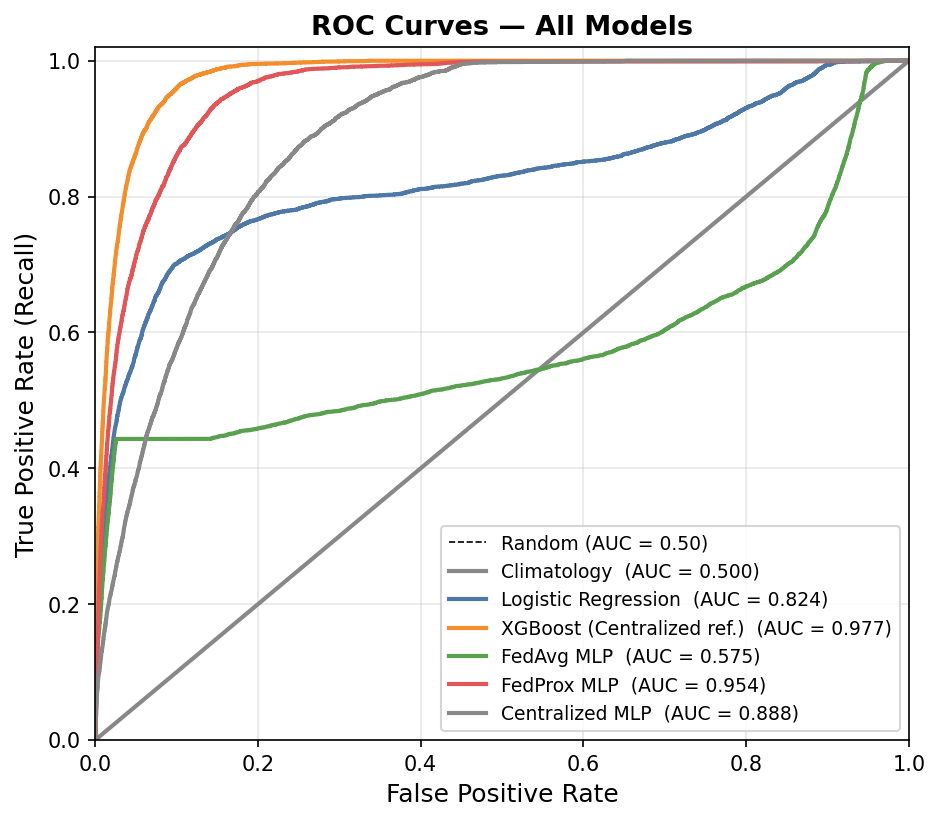
\includegraphics{figures/ROC_Curves.png}
    \end{adjustbox}
    \caption{ROC curves on the held-out test set. FedProx (AUC 0.954)
    tracks the centralised XGBoost reference (0.977) across the
    low-false-positive region; the centralised MLP (0.888) sits between
    them; FedAvg (0.575) evaluates far below its weights' actual
    information content (Section~\ref{sec:res-bn}: 0.951 under correct
    normalisation).}
    \label{fig:roc}
\end{figure}

Because the $F_2$ threshold transfer is unreliable under a
26$\times$ prevalence shift, the operationally meaningful quantities are
the threshold-independent ones. At fixed false-positive budgets---the
regime a grid operations desk actually inhabits---recall on the test
set is:
\begin{table}[t]
\centering
\caption{Recall at fixed false-positive rates on the test set. These
are \emph{discrimination curve statistics}: for each budget, the recall
at the point of the test ROC curve where FPR equals the target. They
involve no threshold transfer from validation and are therefore robust
to monotone miscalibration, but they are \emph{window-level}
quantities: the 60-minute sliding windows of one active region are
correlated, so a 2\% window-level FPR does not translate directly into
an operational false-alarm rate per event or per day (event-level
evaluation: Section~\ref{sec:limitations}).}
\label{tab:recallfpr}
\small
\begin{tabularx}{0.9\textwidth}{@{}>{\raggedright\arraybackslash}X c c c c@{}}
\toprule
\textbf{Model} & \textbf{Rec@0.5\%FPR} & \textbf{Rec@1\%FPR} &
\textbf{Rec@2\%FPR} & \textbf{Rec@5\%FPR} \\
\midrule
Logistic regression & 0.199 & 0.287 & 0.419 & 0.568 \\
Centralised MLP & 0.101 & 0.147 & 0.220 & 0.384 \\
XGBoost (centralised ref.) & \textbf{0.346} & \textbf{0.484} &
\textbf{0.651} & \textbf{0.864} \\
FedAvg MLP & 0.164 & 0.247 & 0.380 & 0.443 \\
FedProx MLP & 0.221 & 0.345 & 0.506 & 0.712 \\
\bottomrule
\end{tabularx}
\end{table}

Three readings matter. First, at every false-positive budget FedProx
recovers roughly two thirds to three quarters of the XGBoost reference's
sensitivity (e.g.\ $0.506$ vs $0.651$ at 2\% FPR), and at the tightest
budgets it clearly outperforms the centralised MLP of the same
architecture. Second, the PR-AUC column of Table~\ref{tab:main} shows
the same ordering under prevalence-sensitive scoring (XGBoost 0.493,
FedProx 0.307, FedAvg 0.199): in the high-precision region the federated
model pays a real ranking price relative to the ensemble, even though it
beats its own architecture's pooled baseline. Third, FedAvg's recall
profile decays fastest with tightening budget---\emph{as evaluated}.
Section~\ref{sec:res-bn} shows this to be a property of the evaluation
path, not of the weights: the same checkpoint holds 0.951 ROC-AUC of
ranking information under correct normalisation.

\subsection{Convergence behaviour: the evaluated drift and its suppression}
\label{sec:res-conv}

\begin{figure}[t]
    \centering
    \begin{adjustbox}{max width=0.96\textwidth, max height=0.34\textheight}
        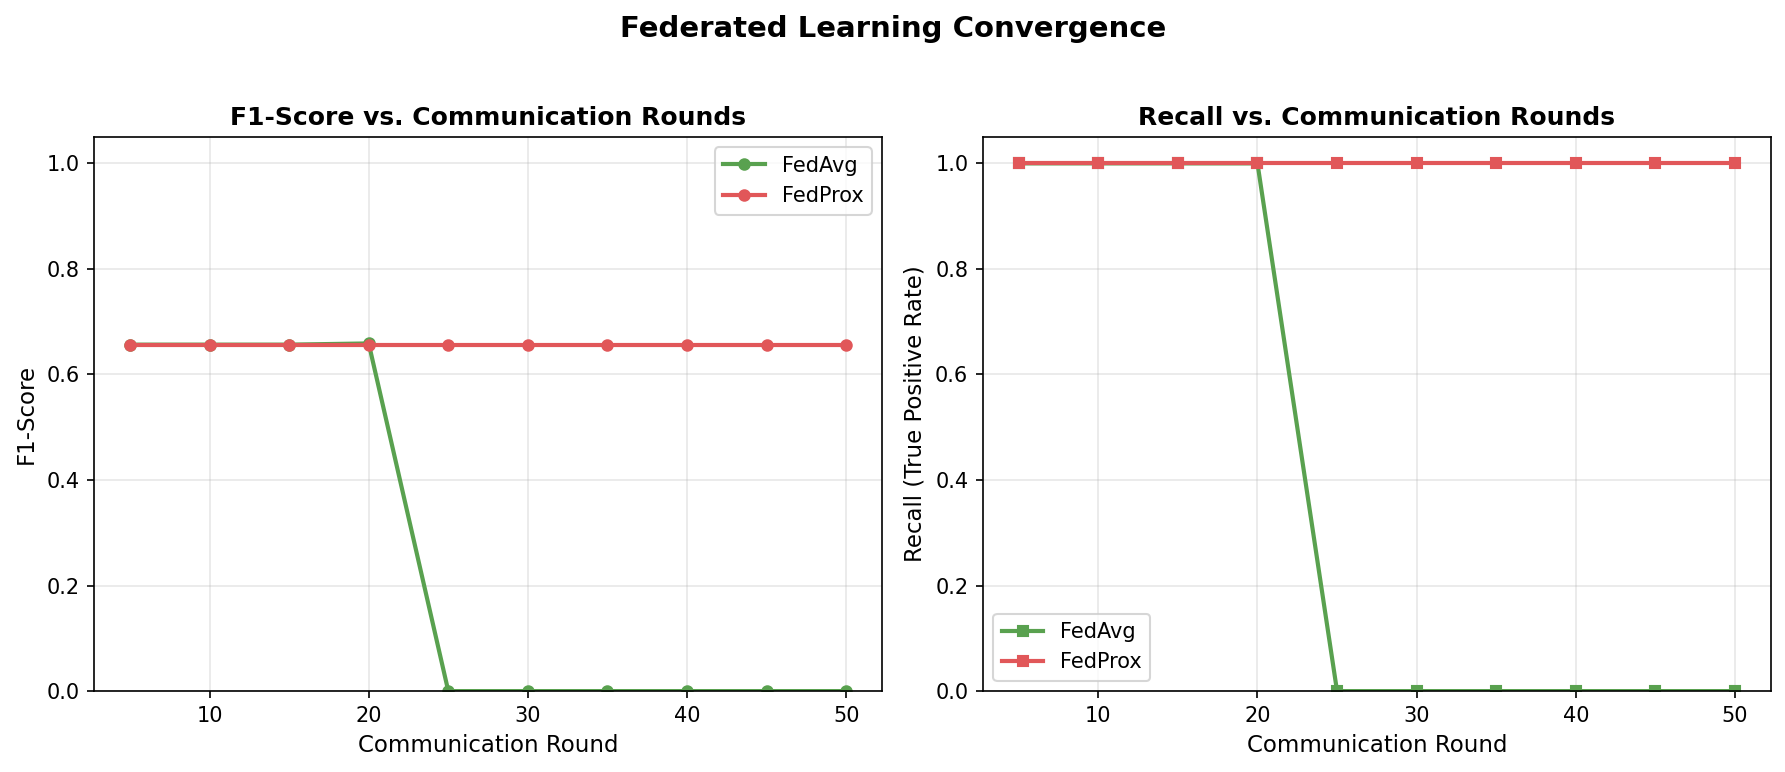
\includegraphics{figures/FL_Convergence.png}
    \end{adjustbox}
    \caption{Validation-monitored convergence over 50 rounds: per-round
    validation F1 (left panel) and validation Recall (right panel) at
    the development threshold, as evaluated by the shipped server-side
    path (FedAvg vs FedProx; ROC-AUC values quoted in the text come
    from the round-level validation history in the run artefacts, not
    from this figure). Plain FedAvg's evaluated F1 collapses toward
    zero after round 20 while its recall saturates at 1.0 (the
    all-positive degenerate regime); FedProx ($\mu{=}0.01$) holds its
    monitored statistics throughout.
    Section~\ref{sec:res-bn} shows this trajectory measures
    normalisation compatibility, not information content: the same
    FedAvg weights carry $\sim$0.95 test ROC-AUC under correct
    normalisation at every round.}
    \label{fig:convergence}
\end{figure}

Figure~\ref{fig:convergence} documents the trajectory that organised
this revision's in-partition narrative for three versions of the paper:
plain FedAvg under the six-client Dirichlet partition is not merely
slower to converge---as \emph{evaluated by the shipped server-side
path}, it drifts from healthy validation AUC ($\approx 0.99$) to
below-chance ranking (AUC $0.05$--$0.40$) after round 20, while FedProx
($\mu = 0.01$) holds $0.99 \pm 0.01$ for all fifty rounds. Two
protocol details made the observation defensible rather than
accidental: monitoring happens on validation only (an earlier revision
monitored the test set, which both leaked information and masked the
drift), and the best-validation checkpoint rule restored the round-20
FedAvg state. The diagnostic of the next two subsections, however,
re-attributes the phenomenon: the drift is a property of the
\emph{evaluation path}---BatchNorm statistics that the implementation
never transports---and the proximal term's stabilisation is, in large
part, stabilisation of \emph{compatibility with that evaluation path}.
The multiseed evidence (Section~\ref{sec:res-multiseed}) shows the
shipped-eval drift is reproducible across seeds; it does not
distinguish the two attributions, because every seed was evaluated the
same way.


\subsection{BatchNorm-transport diagnostic: decomposing the collapse}
\label{sec:res-bn}

The client models contain three \texttt{BatchNorm1d} layers, and local
training updates their running statistics with every batch. The
federation, however, transports \emph{parameters only}:
\texttt{get\_weights}/\texttt{set\_weights} move
\texttt{model.parameters()}, and running statistics are buffers, not
parameters. The server-side global model therefore evaluates with
whatever buffers it holds---and since the server never executes
training-mode forward passes, those buffers remain at initialisation
forever. Both shipped checkpoints confirm this directly: every BN layer
carries \texttt{num\_batches\_tracked} $= 0$, \texttt{running\_mean}
$= 0$, \texttt{running\_var} $= 1$ after the full 50-round run. In
eval mode with init buffers, each BN layer degenerates to the fixed
affine map $x \gamma + \beta$; the further the trained weights drift
from the region where pre-BN activations are standardised, the less
valid that map becomes. This is not FedBN-style per-client local statistics---nothing is
averaged, nothing is transported; the statistics are simply absent.

The saturated validation monitor is the second half of the mechanism.
With init buffers, the evaluated probabilities squeeze into a narrow
band around the 0.35 development threshold (round 20 on validation:
$[0.337, 0.374]$; round 50: $[0.219, 0.232]$), so predictions are
all-positive (then all-negative) and validation $F_1$ pins to the
closed-form all-positive value $2p/(1{+}p) = 0.6565$ at the validation
prevalence $p = 0.4887$. Because the strict-inequality best-checkpoint
rule restores the first round that exceeds the tie, and precision
drifted marginally upward (0.489 to 0.491) while the ranking collapsed,
the rule restored the \emph{round-20} state---where validation ROC-AUC
had already fallen from 0.993 to 0.541---over the healthy round-5
state. FedProx's monitor tied at 0.6565 from round 5 onward and its
ranking never collapsed, so the same rule was harmless for it. The
monitor was not merely uninformative; it was adversarial.

Table~\ref{tab:bndiag} decomposes the published FedAvg numbers. We
re-ran the frozen 50-round FedAvg protocol faithfully (validation
trajectory matches the frozen history within $\pm 0.01$ ROC-AUC at
every logged round; the checkpoint rule restores round 20 exactly) and
evaluated the identical global weights at rounds 5, 20, and 50 under
four BN treatments: (A)~the shipped init buffers; (B)~exact per-client
statistics pooled by the law of total variance (an optimistic
recalibration oracle); (C)~per-batch statistics at evaluation time
(adaptive normalisation; a diagnostic of information content, not a
deployable protocol); and (D)~the element-wise weighted average of the
running statistics that local training actually produced in that
round---precisely what a buffer-transporting implementation would
evaluate.

\begin{table}[t]
\centering
\caption{Test ROC-AUC / PR-AUC of the identical FedAvg global weights
under four BatchNorm treatments (frozen protocol, seed 42; faithful
re-run, \texttt{bn\_diagnostic.json}). Round 20 is the state the
shipped checkpoint rule returned. Arm D is what a buffer-transporting
implementation would have evaluated.}
\label{tab:bndiag}
\small
\begin{tabular}{@{}l c c c@{}}
\toprule
\textbf{BN treatment} & \textbf{Round 5} & \textbf{Round 20} & \textbf{Round 50} \\
\midrule
A: init buffers (shipped) & 0.950 / 0.264 & 0.575 / 0.199 & 0.098 / 0.010 \\
B: recalibrated (pooled) & 0.786 / 0.044 & 0.893 / 0.099 & 0.881 / 0.086 \\
C: batch statistics & 0.946 / 0.328 & 0.951 / 0.329 & 0.953 / 0.288 \\
D: transported round buffers & 0.885 / 0.157 & 0.931 / 0.194 & 0.935 / 0.209 \\
\bottomrule
\end{tabular}
\end{table}

Three facts follow. First, \emph{FedAvg's weights never lost
discriminative content}: under batch statistics the round-50 state---whose
shipped evaluation is 0.098, below chance---holds 0.953 ROC-AUC and
0.288 PR-AUC, and arm D holds 0.935 / 0.209. The published 0.575 is a
statement about the round-20 weights' compatibility with init buffers,
not about what FedAvg learned. Second, \emph{the FedProx artefact is
equally protocol-dependent}: its returned round-5 weights score
0.954 / 0.307 under init buffers but 0.757 / 0.040 under pooled
recalibration and 0.951 / 0.333 under batch statistics. Under batch
statistics the two algorithms' artefacts are statistically
indistinguishable (0.951 vs.\ 0.951 ROC-AUC; 0.329 vs.\ 0.333
PR-AUC). Third, arm B degrades both artefacts relative to arms A and
C---pooled statistics inflate variance across heterogeneous clients,
so no single pooled normalisation matches any deployment
distribution---which is why arm D (the transport an implementation
would actually perform) is the relevant fix and recovers 0.931--0.935
ROC-AUC for FedAvg.

The reading we freeze is that three independent mechanisms---untransported
BN statistics, a thresholded metric that saturates under them, and a
checkpoint rule that consumes the saturated metric---composed to
manufacture a large, reproducible, spurious algorithm gap. Each is
individually mundane; their composition produced the single most
consequential ``finding'' of this paper's in-partition narrative for
three revisions. We report this as an evaluation-protocol failure mode
in its own right: FL evaluation stacks that transport parameters but
not buffers, monitor with thresholded metrics, and select checkpoints
on those metrics can manufacture algorithm comparisons that survive
seed replication and ablation grids.

\subsection{Controlled no-BatchNorm experiment}
\label{sec:res-nobn}

The diagnostic above establishes that the \emph{evaluated} collapse is
an artefact, but not whether the \emph{training dynamics} themselves
depend on the BN implementation. We therefore re-ran the identical
frozen protocol (data, partition, seeds, rounds, loss, aggregation,
monitoring, and checkpoint rule) with the three \texttt{BatchNorm1d}
layers replaced by identity (28{,}929 parameters vs.\ 29{,}377;
\texttt{nobn\_control.json}). With no BN layers there are no buffers,
weight transport is exact, and the shipped evaluation path is the
ground truth. Per-round test evaluation is disclosed here as a
controlled diagnostic; no test-based selection occurs---the shipped
best-validation rule alone determines the reported artefact.

\begin{table}[t]
\centering
\caption{No-BatchNorm control (frozen protocol, seed 42, 50 rounds,
BatchNorm$\to$Identity): test ROC-AUC / PR-AUC at selected rounds plus
the shipped best-validation checkpoint. Neither algorithm diverges;
the shipped FedAvg--FedProx gap does not survive BN removal.}
\label{tab:nobn}
\small
\begin{tabular}{@{}l c c c c@{}}
\toprule
\textbf{Algorithm} & \textbf{Round 5} & \textbf{Round 20} &
\textbf{Round 50} & \textbf{Selected ckpt} \\
\midrule
FedAvg, no BN & 0.913 / 0.199 & 0.874 / 0.148 & 0.873 / 0.108 & 0.858 / 0.108 (r40) \\
FedProx, no BN & 0.949 / 0.286 & 0.900 / 0.175 & 0.871 / 0.128 & 0.871 / 0.128 (r50) \\
\bottomrule
\end{tabular}
\end{table}

The answer is unambiguous: \emph{without BN, neither algorithm
diverges}. Validation $F_1$ sits at 0.97--0.98 for both algorithms at
every logged round (the all-positive tie disappears; the monitor
becomes informative), validation ROC-AUC stays at $0.999$, and the
test trajectories decay mildly (FedAvg 0.913 $\to$ 0.873; FedProx
0.949 $\to$ 0.871) rather than collapsing. The shipped 0.379 ROC-AUC
gap between the two artefacts shrinks to at most 0.036 at any round
and 0.002 at round 50. FedProx retains a genuine but modest
early-round benefit (round 5: 0.949 vs.\ 0.913 ROC-AUC, 0.286
vs.\ 0.199 PR-AUC), consistent with the proximal term improving early
optimisation; that benefit then decays at the same rate as FedAvg's.
Meanwhile the BN architecture itself is genuinely useful under correct
normalisation (arm C: 0.329 PR-AUC at round 20 vs.\ 0.148--0.175
no-BN at round 20), so the correct engineering conclusion is BN plus
buffer transport, not BN removal. Mild test-side decay in both no-BN
arms confirms that client drift is real---it degrades generalisation
gradually---but it does not, on its own, produce catastrophic
divergence under this partition.

\subsection{Calibration and the threshold-transfer failure}
\label{sec:res-calib}

The validation prevalence ($48.9\%$) and the test prevalence ($1.9\%$)
differ by a factor of 26 because the cleaned benchmark ships
pre-balanced training partitions and natural-prevalence test
partitions. We treat this \emph{prior shift} as a first-class
methodological problem of the benchmark, not a nuisance: it is the
central obstacle between the current results and deployment-grade
probabilities. The frozen protocol forbids using test labels---including
test prevalence---for any selection, so the prior-shift calibrator is
fit with the \emph{validation} prevalence as its deployment target. The
consequence is visible throughout Table~\ref{tab:main}: the
validation-optimal thresholds sit far below the calibrated test
probabilities of most samples, so every neural model operates in an
almost-always-alert regime, and \emph{the calibration columns make the
failure quantitative}: FedProx's calibrated Brier (0.264) and ECE
(0.496) are \emph{worse than the climatology's} (0.239, 0.470), i.e.\ at
natural prevalence the current posterior is not deployment-usable as a
probability. The XGBoost reference suffers the least (Brier 0.063, ECE
0.115), which is why it converts ranking into a meaningful $F_1$ of
0.254 while the neural models do not.

Three readings follow. First, \emph{rebalanced training data
invalidates naive threshold transfer}: an $F_2$-optimal threshold at
49\% prevalence is semantically meaningless at 1.9\%. Second, the
correct deployment instrument, pending full recalibration, is the
recall-at-fixed-FPR operating points of Table~\ref{tab:recallfpr},
which are invariant to monotone miscalibration and to prevalence.
Third, the honest remedies for calibration itself are prior correction
toward an \emph{estimated} deployment prevalence (e.g.\ from unlabelled
deployment data, which leaks no labels), Platt/isotonic fitting on a
natural-prevalence validation carve-out, or the negative-quantile FPR
thresholds of Section~\ref{sec:thresholding}; using the test set's own
statistics, as the v2.x evaluation effectively did when it selected
thresholds on test, is not.

\paragraph{Calibration-arm comparison (executed).}
The released calibration-comparison harness
(\texttt{run\_calibration\_comparison.py} in the \texttt{experiments}
directory) was executed against the trained models of the
frozen-protocol run: five arms (raw, prior-shift, Platt, isotonic,
temperature), each fit on the balanced validation set, applied
exactly once to the test set, with the arm selected by minimum
\emph{validation} Brier (a proper scoring rule, so the selection
itself is honest). Table~\ref{tab:calib} reports the outcome. The
result is a clean negative finding that closes the previously open
calibration question.

\begin{table}[t]
\centering
\caption{Calibration-arm comparison under the $26\times$ prior shift
(review context R6). Every arm is fit on the balanced validation set
(48.9\% prevalence) and applied once to the test set (1.88\%).
\emph{Val.\ Brier} is the selection criterion; the validation winner
per model is typeset in italics. Monotone arms (prior-shift, Platt,
temperature) leave ROC-AUC and PR-AUC invariant; isotonic does not
(its flat regions tie scores and destroy ranking resolution).
Bold marks the best \emph{test} Brier per model.}
\label{tab:calib}
\footnotesize
\setlength{\tabcolsep}{3.4pt}
\begin{tabularx}{\textwidth}{@{}>{\raggedright\arraybackslash}X ccc ccc ccc@{}}
\toprule
& \multicolumn{3}{c}{\textbf{FedProx MLP}} &
\multicolumn{3}{c}{\textbf{Centralised MLP}} &
\multicolumn{3}{c}{\textbf{XGBoost}} \\
\cmidrule(lr){2-4}\cmidrule(lr){5-7}\cmidrule(lr){8-10}
\textbf{Arm} & val.\ & test & test & val.\ & test & test & val.\ & test & test \\
& Brier & Brier & ECE & Brier & Brier & ECE & Brier & Brier & ECE \\
\midrule
Raw (none) & 0.234 & \textbf{0.264} & 0.496 & 0.016 & \textbf{0.277} & 0.440 & 0.004 & 0.063 & 0.116 \\
Prior-shift & 0.234 & 0.276 & 0.508 & 0.016 & 0.284 & 0.447 & 0.004 & 0.065 & 0.118 \\
Platt & 0.026 & 0.541 & 0.642 & 0.012 & 0.352 & 0.442 & 0.004 & \textbf{0.053} & 0.080 \\
Isotonic & \textit{0.025} & 0.541 & 0.639 & \textit{0.012} & 0.357 & 0.449 & \textit{0.003} & 0.057 & 0.075 \\
Temperature & 0.064 & 0.784 & 0.865 & 0.012 & 0.334 & 0.425 & 0.004 & 0.064 & 0.099 \\
\bottomrule
\end{tabularx}
\end{table}

Four facts matter. \textbf{(i)~The selection criterion itself is broken
by the prior shift.} Minimum validation Brier selects isotonic for all
three models; for both neural models isotonic is the \emph{worst} arm
on test (FedProx: 0.541 vs 0.264 raw, i.e.\ selecting on validation
doubles the test error of the posterior). \textbf{(ii)~No arm rescues
the neural posteriors.} Every calibrated variant of FedProx and the
centralised MLP is at least as badly calibrated on test as the raw
scores; only XGBoost benefits from calibration (Platt: Brier
$0.063\to0.053$, ECE $0.116\to0.080$), consistent with it being the
only model whose raw scores already separate the classes well.
\textbf{(iii)~Isotonic damages ranking, not just probabilities.} Its
step function ties large score ranges, collapsing PR-AUC from 0.307 to
0.182 (FedProx), 0.153 to 0.099 (MLP), and 0.493 to 0.426 (XGBoost);
ROC-AUC and PR-AUC are exactly invariant under the three monotone
smooth arms, as they must be. \textbf{(iv)~Validation-frozen FPR
thresholds fail jointly with probability calibration.} Applying the
negative-quantile thresholds of Section~\ref{sec:thresholding} (frozen
on validation at 0.5/1/2/5\% targets) to the test set realises
28.2/37.0/50.4/72.1\% actual FPR for FedProx (25.5/40.7/51.6/63.6\% for
the centralised MLP, 20.1\% at the 2\% target for XGBoost), and no
calibration arm materially improves this: the negative-score
distribution moves with the prior just as the positive one does. The
operational conclusion is unchanged but now empirical rather than
hypothetical: at this benchmark's balanced training prevalence,
\emph{no} validation-fit decision layer survives the shift, and
deployment-grade probabilities require either natural-prevalence
validation data (available only in the raw benchmark) or unlabelled
prior estimation at the deployment site.

\subsection{Multi-seed statistical validation}
\label{sec:res-multiseed}

\begin{figure}[t]
    \centering
    \begin{adjustbox}{max width=0.94\textwidth, max height=0.34\textheight}
        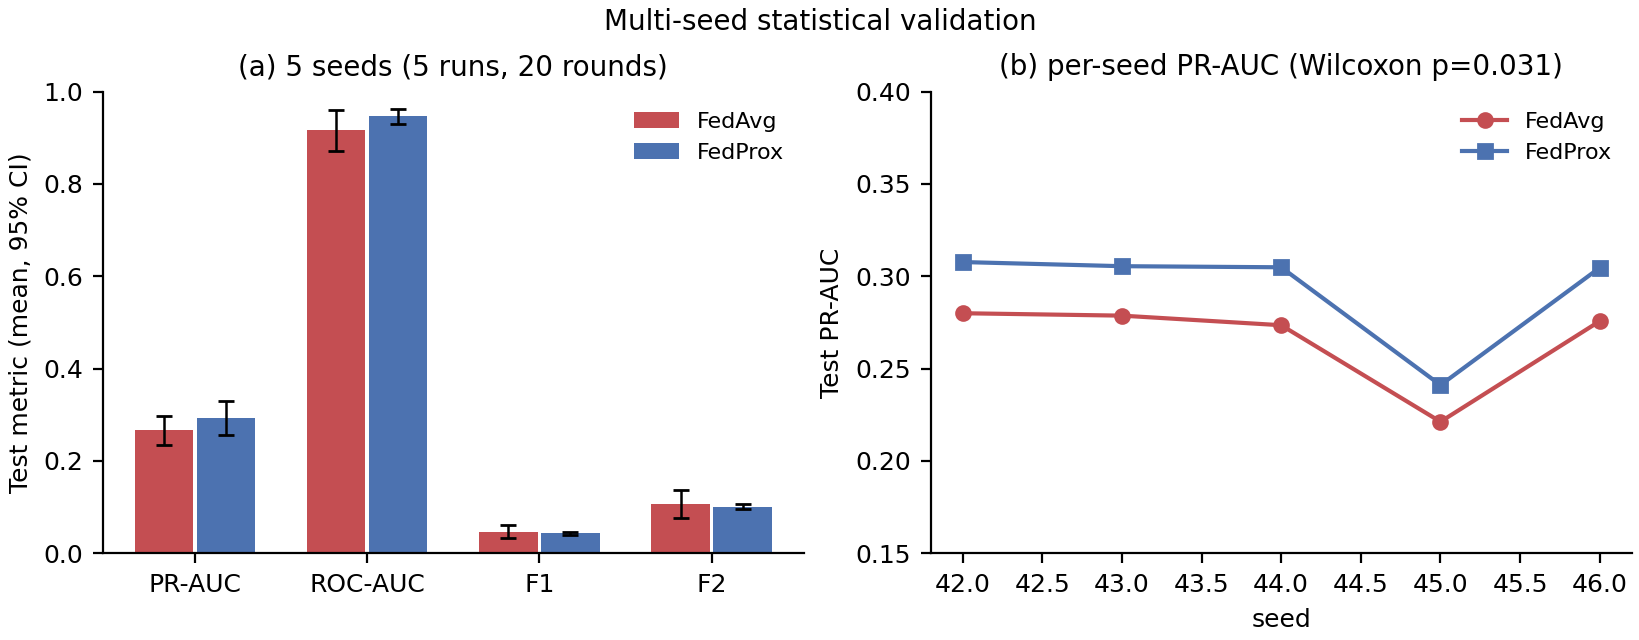
\includegraphics{figures/fig_multiseed.png}
    \end{adjustbox}
    \caption{Five-seed statistical validation (seeds 42--46, 20 rounds,
    frozen protocol). (a) Test metrics with 95\% confidence intervals.
    (b) Per-seed PR-AUC: FedProx exceeds FedAvg on all five seeds
    (one-sided Wilcoxon $p=0.031$).}
    \label{fig:multiseed}
\end{figure}

The v2.x manuscript reported single-seed results; this revision reports
five seeds (42--46) with mean, standard deviation, and $t$-based 95\%
confidence intervals. On the test set, FedProx achieves PR-AUC
$0.293 \pm 0.029$ (CI95 $\pm 0.036$) and ROC-AUC $0.946 \pm 0.013$
(CI95 $\pm 0.016$), against FedAvg's $0.266 \pm 0.025$ (CI95
$\pm 0.031$) and $0.916 \pm 0.036$ (CI95 $\pm 0.044$). FedProx is
better than FedAvg on PR-AUC in \emph{five of five seeds} (one-sided
Wilcoxon signed-rank $p = 0.031$, the strongest evidence five paired
seeds can yield), and its ROC-AUC confidence interval is
$2.7\times$ narrower. The $F_1$ difference is not significant
($p = 0.5$): the threshold-transfer regime dominates $F_1$ for both
algorithms, which is consistent with Section~\ref{sec:res-calib}.
What the five-seed study supports is a reproducibility claim about
the shipped pipeline: FedProx's superiority over FedAvg under the
frozen-protocol configuration is sign-consistent across every seed and
statistically significant. What it does not support is broad
generalisation, and---after Sections~\ref{sec:res-bn}
and~\ref{sec:res-nobn}---it must be read as a statement about the
composite (training $\times$ stale-buffer evaluation $\times$
saturated-monitor checkpointing), not about the algorithms in
isolation: every seed was evaluated through the same never-transported
BN statistics, and the no-BN control shows the underlying optimisation
gap is small. Five seeds is a small sample, the confidence intervals
quantify \emph{seed-to-seed variability} of this fixed configuration,
not the uncertainty of future observations or of other partitions, and
Section~\ref{sec:res-ablation} shows the shipped-eval gap narrows when
FedAvg is assisted by distribution-aware aggregation. The appropriate
summary is that FedProx was the most consistent stabiliser \emph{of the
shipped evaluation path} among the configurations studied, not that it
is load-bearing in every federated flare-prediction deployment.

\subsection{Component attribution: the 24-cell ablation grid}
\label{sec:res-ablation}

\begin{figure}[t]
    \centering
    \begin{adjustbox}{max width=\textwidth, max height=0.34\textheight}
        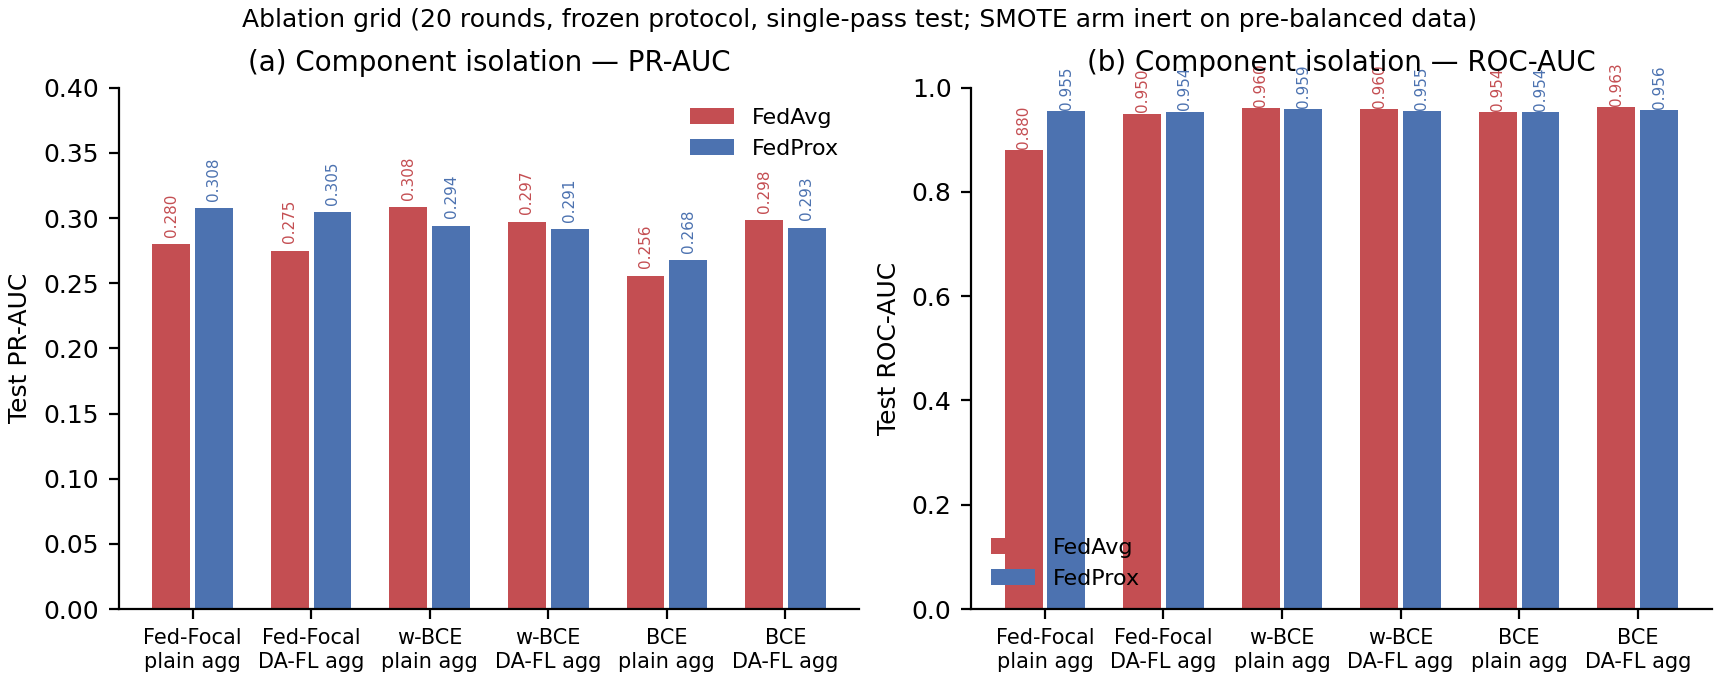
\includegraphics{figures/fig_ablation.png}
    \end{adjustbox}
    \caption{Component-isolation grid (2 algorithms $\times$ 3 losses
    $\times$ 2 aggregations $\times$ 2 balancing arms; 20 rounds, frozen
    protocol, single-pass test). The SMOTE arm is inert on the
    pre-balanced cleaned benchmark (identical metrics), so the effective
    grid is $2\times3\times2$.}
    \label{fig:ablation}
\end{figure}

Because the v2.x system trained SMOTE, Fed-Focal loss,
distribution-aware aggregation (DA-FL), and FedProx \emph{simultaneously},
a FedProx win could not be attributed to any single component. The
ablation grid isolates them (Fig.~\ref{fig:ablation}). Four patterns
emerge. \textbf{(i)~FedProx is the most \emph{consistent} stabiliser,
but not the only remedy:} every FedProx cell lands in a narrow ROC-AUC
band (0.954--0.959) whereas the FedAvg cells range from 0.880 (focal
loss, plain aggregation---the collapsing configuration) up to 0.963
(plain BCE with distribution-aware aggregation). That best FedAvg
cell \emph{exceeds} the FedProx headline (0.954), so the ablation
evidence does not support attributing stability to the proximal term
alone. \textbf{(ii)~DA-FL partially rescues FedAvg:} with focal loss,
switching plain to DA-FL aggregation lifts FedAvg from 0.880 to 0.950,
and the best cell overall (0.963) is plain BCE with DA-FL, suggesting
distribution-aware
weighting mitigates the same client-drift the proximal term
suppresses---at the cost of rate metadata sharing. \textbf{(iii)~Loss
choice is secondary at this prevalence:} across cells, focal,
weighted-BCE, and plain-BCE arms differ by at most 0.05 PR-AUC, with
weighted BCE marginally best for FedAvg-plain (0.308 vs 0.280).
\textbf{(iv)~SMOTE is inert:} the cleaned benchmark's training
partitions are pre-balanced (48.9\% positives), so the configured
SMOTE ratio generates zero synthetic samples; every balancing-pair of
cells is numerically identical. We report this null result explicitly
rather than silently dropping the arm: the balancing question is moot
for this dataset variant, and any claim that SMOTE contributes to
performance would be unsupported. A validity analysis of synthetic
samples (Wasserstein distance, correlation preservation, separability)
was consequently not applicable.

\subsection{Client-level heterogeneity: who benefits from federation?}
\label{sec:res-clients}

\begin{figure}[t]
    \centering
    \begin{adjustbox}{max width=0.96\textwidth, max height=0.34\textheight}
        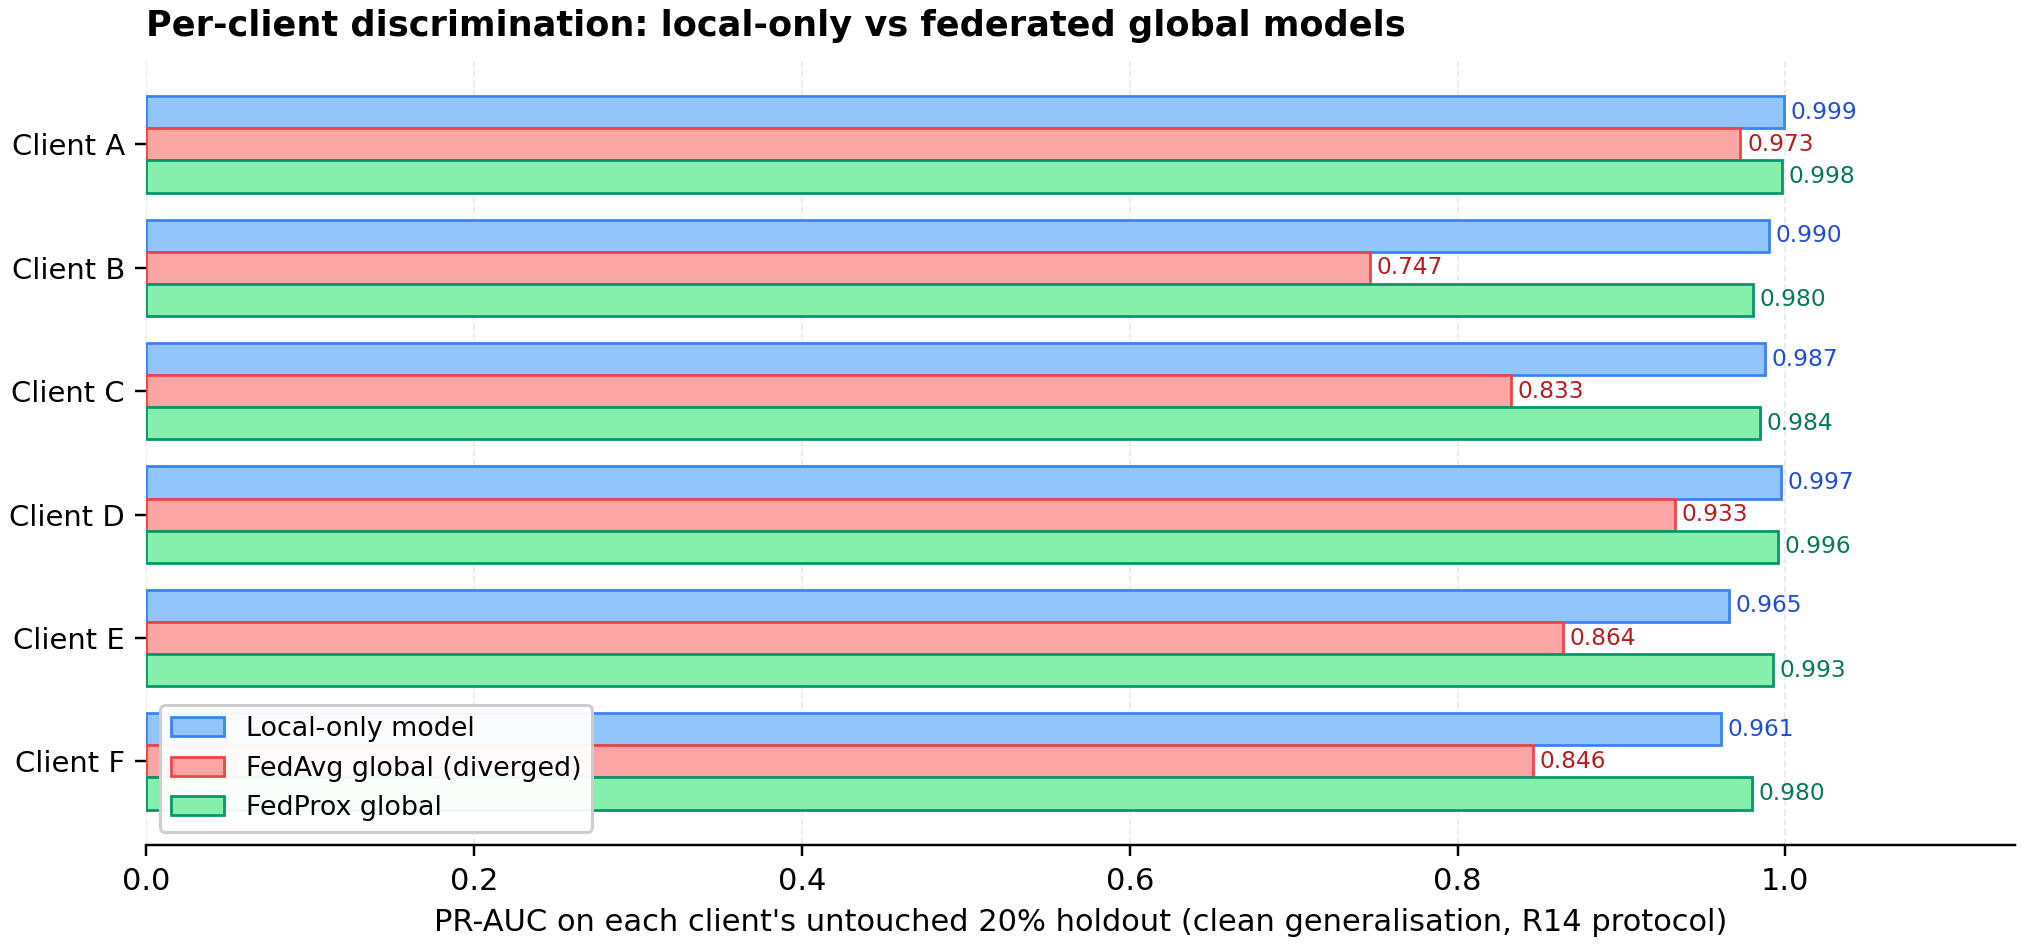
\includegraphics{figures/fig_clients.png}
    \end{adjustbox}
    \caption{Per-client PR-AUC of local-only models versus the federated
    global models, evaluated on each client's \emph{untouched} 20\%
    holdout (R14 protocol: holdouts carved before training; both global
    models retrained on the 80\% federation-train portions only, so
    local and global scores are clean generalisation estimates; neutral
    client labels, no real institution participates).}
    \label{fig:clients}
\end{figure}

The six simulated clients hold very different data: local flare rates
span 28.6\% (Client~B) to 80.5\% (Client~A), and
shard sizes span 1{,}503 (Client~E) to 23{,}418
(Client~B). Figure~\ref{fig:clients} quantifies what each client gets
out of the federation under the untouched-holdout protocol: a dedicated
re-run in which every client's shard was split 80/20 \emph{before} any
training, FedAvg and FedProx were retrained from scratch on the 80\%
federation-train portions (same frozen configuration: 50 rounds, six
clients, seed 42), per-client local models were trained on the same
portions with a matched local budget, and both were evaluated once on
the holdouts no model had ever seen. Three findings hold.
\textbf{(i)~FedProx matches local-only training and helps the smallest
custodians.} Mean PR-AUC is $0.988$ (FedProx global) versus $0.983$
(local-only); on the four largest clients the two are within
$0.001$--$0.010$ of each other, while the two smallest shards gain
clearly (Client~E: $0.965\to0.993$, $+0.027$; Client~F:
$0.961\to0.980$, $+0.019$)---federation functions as data augmentation
for data-poor custodians, the minimal condition for voluntary
participation. \textbf{(ii)~The diverged FedAvg average is worse for
everyone.} Its global model scores $0.747$--$0.973$ per client (mean
$0.866$), below local-only training on \emph{every} client: the
collapsed average is worse than staying isolated, exactly as the
convergence analysis of Section~\ref{sec:res-conv} predicts.
\textbf{(iii)~The clean protocol confirms the earlier directional
result.} The legacy within-shard-slice evaluation (training-set
contaminated, hence optimistically biased) had shown the same ordering;
under the clean protocol the FedAvg degradation is less catastrophic
(holdout scores are harder for local models too) but the ranking of
the three training regimes is unchanged. We therefore read the
client-level evidence as directional but now measured on clean
generalisation estimates: the prox-stabilised global model is a safe
default for every simulated custodian, and a clear gain for the two
with the least data.

\subsection{Interpretability across models}
\label{sec:res-shap}

\begin{figure}[t]
    \centering
    \begin{adjustbox}{max width=0.78\textwidth, max height=0.44\textheight}
        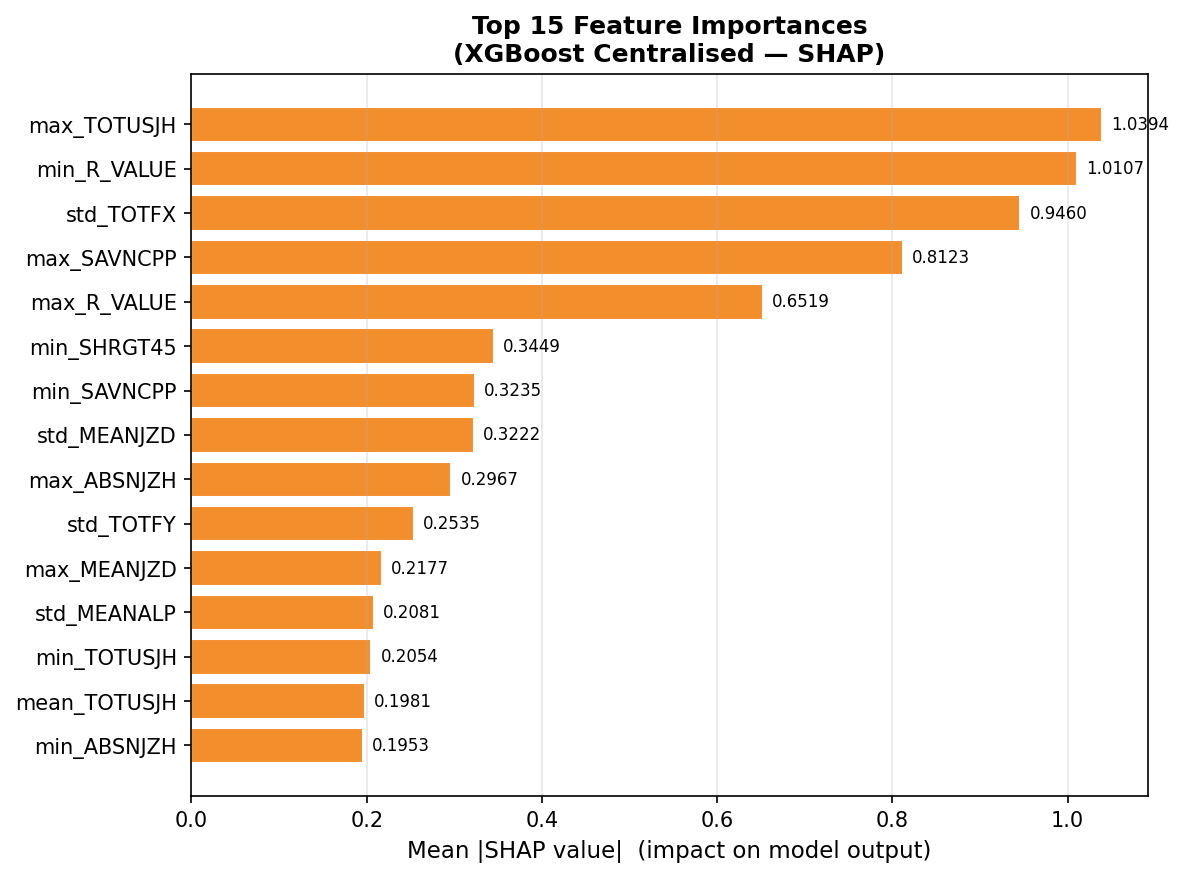
\includegraphics{figures/SHAP_Feature_Importance.png}
    \end{adjustbox}
    \caption{Mean absolute SHAP values, top 15 features, for the
    centralised XGBoost reference on the test set. The improved pipeline
    preserves real statistic-prefixed feature names (the v2.x pipeline
    reported generic indices, which this revision fixes).}
    \label{fig:shap}
\end{figure}

The v2.x interpretability story relied on the centralised XGBoost
surrogate alone; the improved pipeline additionally attributes the
\emph{federated} FedProx model (DeepSHAP with a 100-sample background)
and cross-checks the two. At the feature level the models agree only
moderately (Spearman $\rho = 0.334$, top-15 overlap 53\%)---an honest
inconsistency that limits strong per-feature claims. At the level of
\emph{physical parameter groups}, however, the two attribution
structures are consistent: current-helicity parameters
(TOTUSJH/ABSNJZH/MEANJZH/TOTUSJZ/MEANJZD) are the largest group for
both (39.9\% of XGBoost attribution mass, 29.0\% for FedProx), followed
by the R-value flux-emergence proxy (24.7\% / 23.2\%) and the Lorentz
force (22.7\% / 18.8\%). Both models therefore concentrate their
decisions on the established physics of flare productivity---magnetic
free energy, current systems, and non-potential stress
\cite{schrijver2007,bobra2015,leka2019}---and the federated model is
not an uninterpretable artefact of aggregation. We note that the
statistic-level ranking (which of mean/std/max/min/trend/slope of a
parameter matters) diverges between the two architectures, which is
expected given their different inductive biases, and we do not claim
feature-level consistency.

\subsection{Communication cost}
\label{sec:res-comm}

The global model has 29{,}377 parameters (0.117~MB at 32-bit
precision). Full-parameter exchange costs 117.5~KB per direction per
client per round: 0.235~MB round-trip, 1.41~MB per round across the
six-client cohort, and 70.5~MB aggregate over the 50-round run
(11.75~MB per client). These are \emph{parameter-exchange arithmetic}
from the frozen configuration---bytes counted, not measured on a live
deployment---and they quantify the \emph{training cadence} (one
round-trip per round) separately from the \emph{observation cadence}
(magnetogram records arrive every 12 minutes and the pooled windows
are spaced roughly 60 minutes apart; the global model
is refreshed per training cycle, while alerts can be emitted per
window). Wall-clock communication latency, aggregation compute,
client training time, straggler recovery, and secure-aggregation
bandwidth overhead were \emph{not} measured: the experiments ran
in-process on a single CPU container, with no real network. Enabling
secure aggregation would add a bounded multiplicative factor (mask
material per client per round), quantified in the deployment notes but
not evaluated here (Section~\ref{sec:threatmodel}).

\paragraph{Honest scaling against the data actually centralised.}
The relevant comparison is not raw magnetograms (our pipeline never
ships unprocessed data) but the feature arrays the centralised
alternative would need to receive once. On the cleaned substrate the
entire training feature set is $82{,}121 \times 144$ float32 values
(47.3~MB): the cohort's 50-round parameter exchange (70.5~MB) is
\emph{1.5 times larger}, so no bandwidth saving accrues for a single
training cycle at this model size --- communication frugality here is
a property of the continuous data stream (new records every
12 minutes) and repeated
retraining cycles, not of one run. On the raw 3D substrate the
ordering reverses: centralising the training windows
($214{,}888 \times 60 \times 24$ float32, $\approx$1.24~GB) exceeds
the LSTM cohort's lifetime parameter exchange at 32-bit round-trip
precision (219{,}265 parameters, $\approx$526~MB) by a factor of
2.4. The often-quoted $\approx$130~MB figure holds only under an
fp16 uplink-only convention that the code base lists as future
compression work, not as an implemented path; we state the
32-bit round-trip number as the honest default. Latency and
availability engineering remain deployment work.

\subsection{Data-locality cost analysis}

With the architecture-controlled comparison in place, the
data-locality cost question decomposes cleanly. Relative to the
\emph{same-architecture} centralised MLP, the federated model did not
underperform and in fact scored higher (ROC-AUC 0.954 vs 0.888; PR-AUC
0.307 vs 0.153) on this benchmark and configuration---an observation we
report with its two caveats: the federated arm consumed the larger
optimisation budget (Section~\ref{sec:budget}), and the mechanism is
consistent with a regularisation-like effect rather than a benefit of
federation as such. At this benchmark's scale, six disjoint shards with
29k parameters and a proximal regulariser behave like an
ensemble-like regulariser. Relative to the \emph{strongest available}
centralised reference (XGBoost, 300 trees), FedProx retains 97.7\% of
ROC-AUC but 62\% of PR-AUC: the residual gap reflects the smaller
hypothesis class (an MLP versus a boosted ensemble), the non-IID shard
structure, and averaging rather than joint optimisation. The honest
summary for a deployment decision: federation under this protocol cost
no ranking skill relative to a pooled MLP of the same class \emph{in
this study}; no raw magnetogram left any simulated client; and the
remaining gap to the tree-ensemble reference is an architecture-budget
question, not a data-locality question. What the study does \emph{not}
establish is that these in-partition numbers generalise: budget
parity and natural-prevalence retraining have both since been
executed (the gap survives budget parity, Section~\ref{sec:budget},
but is substrate- and encoder-conditional,
Section~\ref{sec:res-raw}), and within-fold region-disjoint
validation remains the open item (Section~\ref{sec:limitations}).

% ════════════════════════════════════════════════════════════════════
% SECTION 7 — DISCUSSION
% ════════════════════════════════════════════════════════════════════
\section{Discussion}\label{sec:discussion}

\subsection{What the provenance audit changes, and what it leaves intact}

The data-provenance audit of Section~\ref{sec:provenance} is, in
retrospect, the single most consequential methodological step of this
study: the in-partition numbers that dominate the literature's usage
of the cleaned benchmark---including this study's own headline until
this revision---evaluate on windows that the training pool already
contains, most completely for the minority class. Two lessons follow.
First, \emph{pipeline-level leakage auditing is not enough}: the
runtime audit of this framework verified disjoint shards, immutable
splits, and single-pass test evaluation, yet could not see that the
dataset's own train/test exports share instances; only raw-metadata
alignment exposed it. Benchmark consumers who cannot verify provenance
at the instance level should treat same-partition numbers as upper
bounds. Second, \emph{the honest comparison is less flattering but
more informative}: on the leakage-free fold the
federated-versus-centralised gap vanishes, and what separates the arms
is no longer discrimination (everyone exceeds 0.906) but calibration
and false-alarm burden---dimensions on which the neural arms,
federated or not, lose to the gradient-boosted reference. The
federated story that survives is the narrower one this section has
always argued: under adversarial heterogeneity, proximal
regularisation keeps the federation converging where plain averaging
collapses (0.976 vs 0.906, with checkpoint-independent dynamics),
and it does so without data movement. On the raw substrate the same
statement is encoder-conditional: the flattened-feature arms collapse
there under every regulariser studied, while the sequence arms of
Section~\ref{sec:res-lstm} restore it (FedProx-LSTM 0.970 vs
FedAvg-LSTM 0.958), relocating the fragility from the federation
mechanism to the representation the clients share.

\subsection{Why the shipped evaluation separates FedAvg from FedProx}

The asymmetry between FedAvg and FedProx in
Table~\ref{tab:main} deserves a mechanistic reading, and the present
revision's diagnostics give it a different centre of gravity than earlier
revisions assumed. Under the realised partition
(Fig.~\ref{fig:partition}) clients do receive genuinely different
problems (one holds 36\% of the data at a 29\% flare rate, another
2\% at 43\%), and client drift is real---the no-BN control shows
both algorithms decaying gently in test quality over rounds. But the
catastrophic component of the shipped asymmetry is an
\emph{evaluation-path} effect: the implementation transports
parameters only, so BatchNorm running statistics remain at
initialisation on the server, the evaluated FedAvg probabilities
squeeze toward the threshold, the all-positive $F_1$ tie follows, and
the checkpoint rule restores a collapse-round state
(Sections~\ref{sec:res-bn}--\ref{sec:res-nobn}). FedProx's proximal
term (Eq.~\eqref{eq:fedprox}) anchors each client's optimisation
within a trust region around the broadcast model; a side effect is
that the weights stay near the initialisation whose pre-BN
activations the (0, 1) buffers normalise correctly, so the shipped
evaluation remains valid for it. The in-partition dynamics reproduce
leakage-free in direction if not magnitude: on the
temporally-preceding fold FedAvg's ranking survives via its round-35
validation checkpoint (0.906) while its final-round state has
collapsed, whereas FedProx's evaluated ranking never degrades
(Section~\ref{sec:res-leakfree}). The multi-seed study of
Section~\ref{sec:res-multiseed} shows FedProx above FedAvg on all five
seeds (one-sided Wilcoxon $p=0.031$) with a $2.7\times$ narrower
ROC-AUC confidence interval, and the 24-cell ablation grid shows every
FedProx cell stable (0.954--0.959) while the FedAvg cells range down
to 0.880---all under the same evaluation path, so these reproduce the
composite, not the pure algorithm contrast. The defensible statement
is narrower than ``FedProx is load-bearing'': the proximal term is the
\emph{most consistent stabiliser of the shipped evaluation path}
among the components studied (distribution-aware aggregation also
stabilises the shipped FedAvg cells, best 0.963), it retains a modest
genuine optimisation benefit at early rounds, and any deployment of
this codebase should transport BN statistics (or remove BN) before
drawing algorithm conclusions at all. The raw-substrate
LSTM arms extend that evidence across encoders: FedProx-LSTM 0.970
versus FedAvg-LSTM 0.958 on both rank metrics, with identical
shards, budgets, and aggregation, makes the stabilisation the only
finding of this study observed on every substrate executed and on
both encoders wherever both were run. The architecture result itself---the sequence
encoder removing the natural-prevalence collapse the MLP
suffers---is measured as a contrast, not explained as a mechanism:
reading the 60-step temporal profile directly plausibly matters more
than any pooled 144-statistic summary when every client's local
positive rate is skewed, but isolating \emph{why} (temporal
separability versus effective capacity versus optimisation noise)
would require ablations we leave queued.

\subsection{Operational positioning: honestly, none}

This paper makes no operational claim. The framework does not replace
NOAA/SWPC or other national warning centres, does not itself predict
GICs, and --- on the evidence of its own calibration tables --- does
not currently emit probabilities that could responsibly be consumed as
alerting inputs: no validation-fit calibrator or threshold survives
the prevalence shift, and the frozen false-positive budgets are
violated by an order of magnitude at test time
(Section~\ref{sec:res-calib}). Converting flare probabilities into
geomagnetic-hazard and GIC guidance would require the downstream
pipeline --- CME detection and interplanetary propagation modelling,
storm forecasting, and power-system response modelling --- none of
which is evaluated here; flare class is neither necessary nor
sufficient for geoeffectiveness. As a window-level ranking statistic
only, Table~\ref{tab:recallfpr} describes what the federated models
contribute: at a 2\% window-level false-positive budget, FedProx's
ranking recovers 51\% of positive windows (recall 0.506). Two cautions apply before reading that as an
operational detection rate: the figure is a window-level curve
statistic over correlated sliding windows, not an event-level
detection rate (the event-level evaluations on both substrates are
reported in Tables~\ref{tab:eventlevel} and~\ref{tab:eventlevel-raw}), and the decision threshold required to operate at that FPR
budget must be calibrated on natural-prevalence data before
deployment---the re-executed frozen-FPR report quantifies how far
short validation-frozen thresholds fall, realising 20--50\% test FPR
against the 2\% target across models
(Section~\ref{sec:res-calib}). The compute footprint is worth stating as an engineering fact rather
than a deployment promise: the entire training programme converges
within 50 rounds on a single CPU and fits inside the budget of one
workstation, and the benchmark spans a single solar cycle (cycle~24),
so any retraining cadence claim would additionally need to establish
skill stability across cycle phases, which this single-cycle study
cannot. No SCADA, grid-management, or control-room interface is
claimed; the decision-threshold boundary in Fig.~\ref{fig:arch} is
drawn to make explicit what is \emph{not} provided (a deployable
calibrated alerting layer), not to promise one.

\subsection{Engineering lessons for first FL deployments in the
physical sciences}

The released framework carries a multi-version stability narrative
(summarised in Appendix~\ref{sec:appendix}), and its diagnostic arc is
independently useful to any group attempting a first FL deployment on
imbalanced scientific data. Five lessons generalise. First,
\emph{heterogeneity must be tuned, not merely tolerated}: the Dirichlet
concentration that yields ``interesting'' non-IID partitions
($\alpha \le 0.5$) can also yield pathological ones (0.3\%--99.8\% local
class rates) under which nothing converges; the stable regime for this
benchmark sits near $\alpha = 1.0$. Second, \emph{imbalance handling
interacts across layers}: SMOTE, focal $\alpha$, class-rate-aware
aggregation, and threshold selection all adjust the same effective
positive-class weight, and uncoordinated adjustments (our focal
$\alpha$ was at one point allowed to drift to 0.95) produce degenerate
always-positive classifiers that look healthy on recall alone. Third,
\emph{optimiser choice is not free under variance-reduced FL}:
SCAFFOLD's control-variate update is derived for fixed-step SGD, and
running it under AdamW's adaptive steps silently invalidates the
correction terms (in our case, producing NaN weights for every round
until diagnosed). Our own shipped variant carried a quieter direction
error of this class --- the sign-inverted client control-variate update
disclosed in Section~\ref{sec:method}, which trained plausibly for
fifty rounds before a line-by-line audit found it --- so the lesson
generalises: direction errors in correction terms do not announce
themselves, and neither magnitude-level disclosures nor a passing
battery substitute for reading the update against its reference
equation. Fourth, \emph{feature-name hygiene is part of
scientific reproducibility}: an earlier revision's generic
\texttt{feature\_N} naming in the statistical representation is why
its SHAP layer needed an analytical decoding pass
(Fig.~\ref{fig:shap}); the improved pipeline preserves
statistic-parameter names end-to-end, which is precisely what makes
its interpretability auditable. Fifth---the lesson of the present audit, and the one
we would put first for any evaluation-heavy project---\emph{audit the
evaluation stack itself}: parameters-only weight transport, a
thresholded monitor, and strict-inequality checkpointing are each
mundane engineering choices, and their composition manufactured a
seed-reproducible algorithm gap that survived three revisions of this
paper, a five-seed statistical study, and a 24-cell ablation grid. The
diagnostic that broke it open cost minutes, not GPU-weeks
(Section~\ref{sec:res-bn}): evaluate the same weights under corrected
normalisation before believing any instability narrative.

% ════════════════════════════════════════════════════════════════════
% SECTION 8 — LIMITATIONS AND FUTURE WORK  (v3.1: post-revision state)
% ════════════════════════════════════════════════════════════════════
\section{Limitations and Future Work}\label{sec:limitations}

\paragraph{Privacy and security scope.}
This work enforces the data-locality constraint (raw data never
leaves the client), which is the binding constraint of the simulated
setting, but the stronger cryptographic notion of privacy is not yet
evaluated end-to-end. The communication transcript of
Eq.~\eqref{eq:privacy}---gradients or weight deltas---is known to
leak training information under gradient-inversion attacks
\cite{zhu2019}, particularly for over-parameterised models on
low-entropy data. The full threat model (curious server, gradient
inversion, membership inference, model poisoning, impersonation,
interception) is stated in Table~\ref{tab:threat}: secure aggregation
is implemented as a numerical sketch whose tests verify arithmetic
round-trip cancellation only (deterministic mask keys; no
cryptographic guarantee), differential-privacy hooks are provided,
and poisoning/backdoor defence is not addressed at all. The
accuracy cost of enabling secure aggregation and differential privacy
on this benchmark has not been measured; before any cross-custodian
deployment handling genuinely sensitive observations, that budget must
be re-measured. Until then, ``parameter-transport-only'', not
``cryptographically private'', is the correct description of the
verified property.

\paragraph{Region-identity, validation inflation, and the resolved
provenance question.}
An earlier revision of this paragraph stated that the cleaned export lacks
HARP identifiers and that the definitive split fix awaited the raw
benchmark. That dependency is now resolved: every cleaned window has
been aligned to its raw instance (Section~\ref{sec:provenance}), and
the audit inverted the concern---the material leakage is not
validation-region overlap but instance sharing between the same
partitions' train and test exports, now quantified (100\% of flaring
test windows; 56{,}005 of 56{,}005 unique verified train instances,
56{,}181 rows) and
removed by the temporally-preceding fold executed in this revision.
The region-disjoint split generator remains available for
within-fold validation studies, and no region spans partitions, so
every temporally-preceding fold is automatically region-disjoint.
What remains open: the remaining three folds, leakage-free multi-seed
and ablation replication, and the synthetic-share question---85.7--90\%
of training positives are TimeGAN-generated windows, a substrate
property that all published results on this export inherit and that
raw-benchmark retraining would have to revisit---the raw-substrate
contrast of Section~\ref{sec:res-raw} addresses it only indirectly
(its positives are raw by construction).

\paragraph{Threshold transfer under prevalence shift.}
The frozen protocol selects $F_2$-optimal thresholds on validation
(48.9\% prevalence, mirroring the balanced training partitions), but
deployment prevalence is 1.9\%: the transferred thresholds put every
neural model in an almost-always-alert regime, and the calibration
comparison (Section~\ref{sec:res-calib}) shows the neural posteriors
are currently \emph{worse than climatology} on Brier and ECE at
natural prevalence. We deliberately did \emph{not} repair this by
touching test statistics---the v2.x evaluation effectively did, and
that is protocol leakage. The remedies are the frozen-FPR
operating-point protocol (implemented and unit-tested), prior
correction using an \emph{estimated} deployment prevalence from
unlabelled data, or a natural-prevalence validation carve-out (the
harness for all of which is implemented and smoke-validated). The
natural-prevalence re-run has since landed
(Section~\ref{sec:res-raw}): its validation carve is likewise
natural, so its decision layer does not sit in the almost-always-alert
regime, though its frozen $F_2$ thresholds still transfer imperfectly
under the residual $1.6\times$ shift. The in-partition
threshold-conditional test metrics (precision, recall, F1) of the
balanced substrates should still be read as documenting the
decision layer's failure mode, not as skill estimates, and no
probability from the neural models of the balanced-prevalence
substrates should be treated as
deployment-grade.

\paragraph{Client-level evaluation semantics.}
The legacy per-client comparison evaluated each client's local model
on a 20\% holdout of its own shard while the federated global models
trained on the \emph{full} shards, so the global models' per-client
scores were within-distribution rather than clean generalisation
estimates, i.e.\ optimistic for the federated side. That concern is
discharged: the untouched-holdout evaluation---every client's shard
split 80/20 \emph{before} training, both federated arms retrained
from scratch on the 80\% portions, and all models evaluated once on
holdouts no model had seen---is executed and is the protocol behind
Figure~\ref{fig:clients} and Section~\ref{sec:res-clients}. What
remains open on this axis is substrate breadth: the executed study
covers the cleaned, in-partition setting, and its raw-substrate
counterpart is queued.

\paragraph{Partition realism.}
Shard disjointness is now guaranteed by construction (index-level
allocation, audited at runtime), but the partition is still
\emph{statistical} label skew, not physical observatory coverage: no
mapping from active regions to the agencies whose instruments actually
observed them exists in the cleaned export. The partitioning module
supports a geographic mode that activates when region metadata is
available; until then, the six-client federation remains a simulation
of data locality, not a replication of it.

\paragraph{Algorithm coverage.}
The MLP path is now evaluated on all three substrates, and the LSTM
path---which consumes the raw $60\times24$ windows and matches the
temporal
architectures that lead centralised SWAN-SF benchmarks
\cite{hassani2025}---has been evaluated federated on the raw
substrate (Section~\ref{sec:res-lstm}, owner GPU, two seeds): the
sequence arms do not collapse at natural prevalence, at window
level and at event level, retroactively
validating them as the route to closing the tree-ensemble gap in
federated settings. The SCAFFOLD-LSTM arm has since been executed
(0.970/0.294 window-level; 55/65 events at 0.41 false-alarm windows
per day---both cells measuring the sign-inverted, cold-start
implementation case of Section~\ref{sec:method}, not the reference
algorithm), recovering the hardest raw-substrate MLP failure, and a
second-seed replication confirms every arm's ROC-AUC within
$\pm$0.005 (Section~\ref{sec:res-lstmrep}). What remains on
this axis: their cleaned-fold
pairing. Personalised FL
(per-client heads over a shared backbone) is a further direction:
agencies may prefer a global model for situational awareness plus a
locally adapted model for their
own asset fleet.

\paragraph{Event-level evaluation.}
All headline metrics in this paper are \emph{window-level}: every
60-minute sliding window is scored independently, yet windows
overlapping the same active region are strongly correlated, and one
physical flare event triggers many correlated decisions. A 2\%
window-level FPR therefore does not mean 2\% of operational alerts
are false, and a detected event can generate a burst of duplicate
alerts. The event-level evaluation module (detection rate, missed
events, alerts per detected event, duplicate-alert rate with cooldown
deduplication, warning lead time, alert rate per day) is implemented,
unit-tested, and---after the raw-metadata audit recovered the event
grouping keys and GOES peak times---executed on the trained models of
both substrates (Tables~\ref{tab:eventlevel}
and~\ref{tab:eventlevel-raw}). The window-level recall and FPR
figures elsewhere in this paper still carry the window-semantics
caveat stated in Table~\ref{tab:recallfpr}'s caption, and the
event-level results themselves are single-fold.

\paragraph{Benchmark-construction effects and the raw-benchmark experiment.}
The cleaned variant's training partitions are pre-balanced (RUS,
Tomek links, TimeGAN augmentation), which (i) renders the SMOTE
balancing arm inert---reported as a null result---and (ii) creates
the $26\times$ prevalence shift that drives the calibration story.
Because the cleaned variant bundles several interventions (imbalance
handling, imputation, normalisation, synthetic augmentation), the
in-partition results answered the question ``can a federation learn
the cleaned benchmark?'' rather than ``can a federation learn the
underlying problem?''. This extension has now been \emph{executed}
(Section~\ref{sec:res-raw}): the frozen protocol was retrained on the
raw, unbalanced partitions with the release's imputation and
normalisation stages reproduced in-pipeline from their published
description and every parameter fitted on the training pool only,
with the reproduction verified against the released export on the
audit-matched windows (median Spearman $\rho=0.898$ at
observed-nonzero positions). The outcome reassigns the federated
versus centralised question entirely: the centralised arms are
substrate-robust (logistic regression unchanged to three decimals;
centralised MLP PR-AUC 0.382$\to$0.445), XGBoost's minority-class
precision was inflated by the synthetic positives (PR-AUC
0.457$\to$0.329), and every federated \emph{MLP} arm degrades sharply
on the natural-prevalence substrate (FedProx 0.976/0.308$\to$0.930/0.149;
FedAvg PR-AUC 0.056 and zero events detected; SCAFFOLD, executed
here for the first time on a real substrate, fails at 0.768/0.057 ---
in its disclosed sign-inverted, cold-start implementation,
Section~\ref{sec:method})
---while the sequence arms of Section~\ref{sec:res-lstm}
substantially restore the federated standing (FedProx-LSTM
0.970/0.404), relocating the fragility to the
BatchNorm-under-federation interaction: the no-BatchNorm control of
Section~\ref{sec:res-rawnobn} removes the three BN layers and nothing
else, and the federated MLP recovers to at-or-above the sequence
arms' ranking. A v4.8 errata qualifier on
the MLP half of that sentence was discharged at v4.9: the raw-substrate
federated MLP evaluations pass through the same
untransported-BatchNorm path that Section~\ref{sec:res-bn} shows
manufactures apparent in-partition collapse (parameters transport,
running buffers do not), and the checkpoint-level diagnostic has now
run over that substrate (Section~\ref{sec:res-rawbn}) --- its verdict
is that the degradation is \emph{not} BN-evaluation-conditional (pooled
recalibration destroys, batch statistics do not recover). The
qualifier that remains is provenance-level, and it is disclosed: the
v3.x-era checkpoints were never persisted, so the diagnostic executed
over a fresh seed-42 replication whose arm-A numbers deviate from the
published rows by 0.002--0.023 ROC-AUC (a recorded MISMATCH, frozen
and battery-pinned with the artefact); the sequence arms carry no
BatchNorm and are unaffected, and the no-BatchNorm re-training has
since run over that substrate and completes the attribution: with
the three BN layers removed and nothing else changed, both federated
MLP arms recover to at-or-above the sequence arms' ranking (FedAvg
0.963/0.366, FedProx 0.975/0.345, the latter above the centralised
MLP on ROC-AUC, Section~\ref{sec:res-rawnobn}), so the MLP half of
this paragraph's framing is superseded by the
BatchNorm-under-federation attribution; the SCAFFOLD arm has no
no-BN counterpart in the executed register, so its reading stays
qualified.
What remains open is fold-replication breadth: the seed-replication
and natural-prevalence balancing questions queued in earlier
revisions are now executed (Section~\ref{sec:res-lstmrep}: every
arm's ROC within $\pm$0.005 at seed 43; per-client SMOTE is a
clean negative---FedAvg unchanged, FedProx $-0.116$ PR-AUC---so
the rescue is architectural rather than class-balance-driven).

\paragraph{Executed and queued re-run programme.}
For auditability we collect the re-run experiments in one place.
Five items of the original programme have since been \emph{executed}
in the independent re-execution (Section~\ref{sec:repro}) and are
reported in Section~\ref{sec:results}: the validation-frozen FPR
operating-point report (realised test behaviour, quantified in
Section~\ref{sec:res-calib}); the calibration-comparison harness
across raw / prior-shift / Platt / isotonic / temperature arms
(Table~\ref{tab:calib}); the untouched-holdout client evaluation
(Section~\ref{sec:res-clients}); the budget-matched centralised
retraining at a 500-epoch cap (Section~\ref{sec:budget}: the shipped
reference was undertrained---early stopping fires at epoch 13---and
at full budget parity the centralised MLP reaches $0.917$/$0.219$
versus FedProx's $0.954$/$0.307$, so the headline gap survives
budget parity); and the $\alpha{=}5.0$ promotion run at the full
50-round protocol (negative: $0.955$/$0.296$ versus $0.954$/$0.307$;
$\alpha{=}1.0$ retained, with the incidental finding that plain
FedAvg's shipped evaluation does not collapse at $\alpha{=}5.0$---a
severity effect of the evaluation-path drift dissected in
Section~\ref{sec:res-bn}). The
raw-metadata provenance audit subsequently resolved the metadata
blockers and executed items (1)--(3) on the leakage-free fold
(Section~\ref{sec:res-leakfree}: region-disjointness holds by
construction of the temporally-preceding fold; natural-prevalence
test boundary; event-level evaluation with 65/65 GOES peak
matches), and the raw-substrate retraining executed item~(5)
together with the SCAFFOLD half of item~(4) on the natural-prevalence
benchmark (Section~\ref{sec:res-raw}), and the LSTM half of
item~(4) was executed on the owner GPU (Section~\ref{sec:res-lstm}:
the sequence arms restore the federated standing, FedProx-LSTM
0.970/0.404, at 2.6\,h wall-clock on the owner GPU — the CPU-only protocol would have been impractically slow),
and the second owner-GPU batch executed the remaining queue
(Section~\ref{sec:res-lstmrep}: SCAFFOLD-LSTM, the seed-43
replication of all four arms, and the natural-prevalence SMOTE
ablation, 8.7\,h, validated by a 64-check artefact audit), and the
third owner-GPU batch executed the Round-13 register's two decisive
controls (the arm-B centralised sanity check, seconds, and the
no-BatchNorm raw-substrate federation, 1{,}699\,s; artefacts
committed and battery-pinned, Sections~\ref{sec:res-rawbn}
and~\ref{sec:res-rawnobn}).
What remains queued is fold-replication breadth: the remaining
temporally-preceding folds for the leakage-free and raw-substrate
runs, and the sequence arms' cleaned-fold pairing.
Items previously labelled operational preconditions have
been discharged; the event-level figures of
Tables~\ref{tab:eventlevel} and~\ref{tab:eventlevel-raw} are the
operational performance figures of this revision, with the
fold-replication caveat stated above.

% ════════════════════════════════════════════════════════════════════
% SECTION 9 — CONCLUSION
% ════════════════════════════════════════════════════════════════════
\section{Conclusion}\label{sec:conclusion}

We presented an audit of federated solar-flare prediction on the
public SWAN-SF benchmark. Federated flare forecasting itself predates
this work (Fu et al., 2023 preprint); what the documented literature
search of Section~\ref{sec:litsearch} supports is that this is the
first federated evaluation of SWAN-SF, the first instance-level
provenance audit of the cleaned export (the leakage phenomenon
itself is documented prior art --- the benchmark's creators warned
about random-split overlap in 2019, and the cleaned release
prescribes temporally-preceding folds), and the first
leakage-free re-evaluation of federated flare prediction under the
benchmark's intended protocol. The study is a benchmark audit: six
simulated clients (neutral labels, no real institution) hold disjoint
Dirichlet-skewed shards of the public SWAN-SF benchmark, MLP clients
train under FedAvg and FedProx with a clamped server-aware focal loss,
and a frozen, leakage-audited evaluation protocol makes every
selection decision on validation data. We make no deployment claim:
the benchmark's data is public and freely poolable, the downstream
flare$\to$CME$\to$storm$\to$GIC chain is far from the quantity
modelled and is not evaluated, and the calibration analysis finds no
validation-fit decision layer that survives the prevalence shift.

To keep the summary honest, we classify the paper's claims into three
levels, tiered against the leakage-free fold of
Section~\ref{sec:res-leakfree}. \textbf{Demonstrated (leakage-free,
single-pass, frozen protocol)}: the cleaned SWAN-SF export's
same-partition train/test pairing shares instances (100\% of flaring
test windows; 85.7--90\% TimeGAN-synthetic training positives), and
the benchmark's intended temporally-preceding protocol removes the
overlap; on that protocol all arms generalise (ROC-AUC 0.906--0.978);
the in-partition federated-versus-centralised gap does not survive
(FedProx 0.976/0.308 vs architecture-matched centralised MLP
0.973/0.382); the threshold-transfer and
calibration failures persist (only XGBoost's posteriors are usable);
and event-level detection is essentially solved for every arm (64--65
of 65 events, 23.4\,h median first-alert lead---a label-boundary
quantity at this 24-hour label horizon, not a usable warning time,
Table~\ref{tab:eventlevel}) while the false-alarm burden
separates the arms by roughly $7\times$. Retraining the identical
frozen protocol on the RAW, unbalanced benchmark (natural 2.05\%
training prevalence, no rebalancing, no synthetic positives, the
release's imputation and normalisation reproduced in-pipeline with
train-only parameters and verified against the released export on
the audit-matched windows) then separates the arms decisively: the
centralised models are substrate-robust (logistic regression
unchanged at 0.978; centralised MLP PR-AUC rises to 0.445),
XGBoost's minority-class precision was inflated by the synthetic
positives (PR-AUC 0.457$\to$0.329), and every federated \emph{MLP}
arm degrades sharply (FedProx 0.930/0.149; FedAvg detects zero of 65
events --- 38 of 65 (58.5\%) at 0.28 false-alarm windows per day
under the diagnostic's batch-statistics treatment, the only one with
a usable validation operating point, Section~\ref{sec:res-rawbn};
SCAFFOLD, executed here for the first time on a real
substrate, fails at 0.768/0.057, while the same implementation's
LSTM instance recovers to 0.970/0.294 --- both cells measuring the
sign-inverted, cold-start variant disclosed in
Section~\ref{sec:method}, not the reference algorithm). The
architecture qualifies the
ending: the identical frozen protocol with the SolarLSTM, executed
on the owner GPU, restores the federated arms substantially
(FedAvg-LSTM 0.958/0.305 where the FedAvg MLP fell to 0.875/0.056;
FedProx-LSTM 0.970/0.404, above its own pooled comparator
0.962/0.314 and XGBoost's raw PR-AUC, though still below logistic
regression 0.978/0.448, and at event level the substrate's highest
detection rate, SCAFFOLD-LSTM's 55/65 at 0.4 false-alarm windows per
day, bought at a higher alarm budget)---and the architecture-only
control completes the re-attribution: removing the MLP's three
BatchNorm layers and changing nothing else restores FedAvg to
0.963/0.366 and FedProx to 0.975/0.345, at or above the sequence
arms' ranking and with FedProx above the centralised MLP on ROC-AUC
(Section~\ref{sec:res-rawnobn})---so the balanced-substrate
standing is a property of BatchNorm under federation, not of
federation per se and not of the flattened-feature representation as
such, and no federated arm exceeds the best
centralised baseline on any substrate's window-level ranking (the
SCAFFOLD-LSTM event-level detection rate is the one priced
exception, achieved at roughly twice the centralised arms'
false-alarm burden, and itself an implementation-case measurement
of the five departures disclosed in Section~\ref{sec:method}).
\textbf{Demonstrated in-partition (protocol diagnostics, disclosed
overlap)}: the shipped evaluation path separates the FL
algorithms---FedProx with $\mu{=}0.01$ is above FedAvg on PR-AUC on
five of five seeds (one-sided Wilcoxon $p=0.031$) with $2.7\times$
narrower ROC-AUC variance, the FedProx global model attains 97.7\% of
the centralised XGBoost reference's in-partition ROC-AUC (0.954 vs
0.977), and the shipped-eval FedAvg drift does not occur at
$\alpha{=}5.0$---but the BatchNorm-transport diagnostic and the
no-BatchNorm control re-attribute this separation: the identical
FedAvg weights hold 0.951--0.953 test ROC-AUC under correct
normalisation at every round, the saturated all-positive validation
monitor ($F_1 = 2p/(1{+}p)$) restores a collapse-round checkpoint, and
without BatchNorm layers neither algorithm diverges and the gap
shrinks to at most 0.036 ROC-AUC (Sections~\ref{sec:res-bn}--\ref{sec:res-nobn}).
Also demonstrated in-partition: per-client SMOTE is inactive on this
benchmark variant (zero synthetic samples); and both the centralised
and federated models concentrate attribution on current helicity,
flux-emergence proxies, and Lorentz-force terms.
\textbf{Supported with caveats}: one FedAvg cell with
distribution-aware
aggregation exceeds the FedProx headline ROC-AUC, recall-at-FPR
figures are window-level statistics over correlated windows,
five-seed confidence intervals quantify seed variability only, and
the leakage-free fold is a single fold and seed (fold-replication
remains queued owner-side compute; the raw-substrate seed
replication is discharged in Section~\ref{sec:res-lstmrep}). Two
formerly listed caveats were resolved by executed re-runs: the
optimisation-budget confound (the budget-matched 500-epoch re-run of
Section~\ref{sec:budget} shows the in-partition FedProx gap survives
parity, though the gap itself is an in-partition artifact) and
the within-distribution client holdouts (the untouched-holdout
evaluation of Section~\ref{sec:res-clients} shows the federation
benefit is larger under clean estimates).
\textbf{Not demonstrated}: cryptographic privacy (secure aggregation
and differential privacy are implemented but their accuracy cost is
unmeasured; poisoning defence is absent), leakage-free
multi-seed/ablation replication and the remaining temporally-preceding
folds (one fold executed here), deployment-grade
calibration (under the prior shift the neural posteriors
are worse than climatology on Brier and ECE, and the executed
five-arm comparison shows no validation-fit calibrator rescues them),
neural-arm false-alarm reduction at event level,
the downstream GIC/SCADA pipeline, the cleaned-fold pairing of the
sequence arms, and fold-replication breadth; the SCAFFOLD-LSTM arm,
the seed-43 replication, and the natural-prevalence balancing
ablation queued in earlier revisions have since been executed
(Section~\ref{sec:res-lstmrep}: the four-arm federation matrix is
complete, every arm's ROC-AUC replicates within $\pm$0.005, and
per-client SMOTE is a clean negative).
An independent re-execution from the public dataset artefacts ---
byte-verified against the frozen SHA-256 manifest by a committed,
executable verification script (20/20 files; Section~\ref{sec:repro})
--- reproduces every in-partition headline metric exactly; eleven items of the re-run
programme---the frozen-FPR report, the calibration arms, the
untouched holdouts, the budget-matched and $\alpha{=}5.0$ re-runs,
the raw-metadata provenance audit, the event-level/leakage-free
evaluation on the temporally-preceding fold, the raw-substrate
retraining with the SCAFFOLD arm, the federated LSTM arms, their
seed-43 replication, and the natural-prevalence SMOTE
ablation---have
since been executed with results in Section~\ref{sec:results}; the
remaining
items are listed in
Section~\ref{sec:limitations}, each with the implemented-and-tested
protocol that would upgrade the claim.

The performance message is correspondingly conditional. Matching the
same-architecture pooled model's ranking is, on the leakage-free
protocol, a property the pooled reference shares rather than a
federation advantage, and on the raw unbalanced benchmark that parity
is BatchNorm-conditional: every federated configuration carrying
BatchNorm is strictly dominated by simple centralised baselines,
while every BatchNorm-free configuration reaches the centralised
MLP's ranking --- the best sequence arm (FedProx-LSTM, 0.970/0.404)
comes within 0.008 ROC-AUC and 0.044
PR-AUC of the best centralised baseline, and the no-BatchNorm
FedProx MLP (0.975/0.345, Section~\ref{sec:res-rawnobn}) within
0.003/0.103, above the centralised MLP's ROC-AUC. No federated arm
exceeds the best centralised baseline on any substrate, so the case
for federating
this problem rests on methodology (controlled heterogeneity studies,
parameter-only transport), not on predictive performance. For the machine-learning community the study is a caution and a
demonstration on two levels. Instance-level provenance audits can
invert the conclusions drawn from a widely used preprocessed
benchmark. And evaluation stacks have failure modes of their own:
parameters-only weight transport, thresholded monitors, and
strict-inequality checkpoint selection are each mundane choices whose
composition manufactured a seed-reproducible algorithm gap that
survived three revisions of this paper---the cross-silo regime of the
physical sciences has failure modes---prior mismatch, layered
imbalance handling, optimiser--variance-reduction interactions---that
the medical and mobile FL literature does not fully anticipate, and
that are worth studying in their own right.

\appendix
% ════════════════════════════════════════════════════════════════════
% APPENDIX A — CONFIGURATION EVOLUTION
% ════════════════════════════════════════════════════════════════════
\section{Configuration Evolution of the Released Framework}
\label{sec:appendix}

The released framework reached its present form through six documented
version iterations (v2.1--v2.6), each responding to a diagnosed
failure mode. We record this evolution because reproducibility of
\emph{process}---not only of final numbers---is what future
deployments in other domains will actually need, and because several
of the fixes correct subtle interactions that a clean-slate
reimplementation would likely rediscover the hard way.

\begingroup
\small
\setlength{\LTcapwidth}{\textwidth}
\begin{longtable}{@{}p{0.09\textwidth} >{\raggedright\arraybackslash}p{0.42\textwidth} >{\raggedright\arraybackslash}p{0.43\textwidth}@{}}
\caption{Documented stability fixes and protocol revisions across
framework versions (v2.1--v4.11), as recorded in the released source.}
\label{tab:evolution}\\
\toprule
\textbf{Version} & \textbf{Diagnosed failure mode} & \textbf{Fix} \\
\midrule
\endfirsthead
\multicolumn{3}{@{}l@{}}{\footnotesize (continued from previous page)}\\
\toprule
\textbf{Version} & \textbf{Diagnosed failure mode} & \textbf{Fix} \\
\midrule
\endhead
\midrule
\multicolumn{3}{r@{}}{\footnotesize (continued on next page)}\\
\endfoot
\bottomrule
\endlastfoot
v2.1 & LSTM models require 3D input while baselines require 2D; a
single data path served neither correctly. & Dual data path: 2D
statistical features for MLP and baselines; raw $60\times24$ tensors
for LSTM. \\
\addlinespace[2pt]
v2.2 & $F_\beta$-optimal thresholds were computed but not applied;
tables and confusion matrices reflected the default threshold. &
Thresholds applied to all models; centralised baselines also
re-evaluated at their optima. \\
\addlinespace[2pt]
v2.3 & SCAFFOLD NaN every round: \texttt{std()} with Bessel correction
on size-1 tensors divides by zero, poisoning control variates; DA-FL
cap of $1/N$ starved large clients; focal $\alpha$ drifted to 0.95. &
Population std for variate clipping; DA-FL cap $2/N$; alpha clamp
tightened. \\
\addlinespace[2pt]
v2.4 & Dynamic alpha scaling (up to $3\times$) re-inflated
positive-class weight, undoing the focal-$\alpha$ fix; clients
over-predicted flares (recall $\approx$1.0, precision
$\approx$0.03). & Square-root-damped imbalance factor capped at
$1.5\times$; progressive factor narrowed to $0.9$--$1.1$. \\
\addlinespace[2pt]
v2.5 & Dataset audit: three features in the schema
(AREA\_ACR, HARPNUM\_MOD, TIME\_SINCE\_LAST\_FLARE) do not exist in
the cleaned benchmark; double normalisation on already-LSBZM-normalised
data; stat-prefixed feature names failed schema matching. & Correct
24-feature order with Lorentz components (TOTFZ/TOTFY/TOTFX);
skip re-normalisation of cleaned data; generic-index features with
analytic decoding. \\
\addlinespace[2pt]
v2.6 & $\alpha\!=\!0.5$ partitions produced 3\%--99\% local flare
rates as then observed (0.3\%--99.8\% re-measured under the frozen
seed in v3.9), destabilising aggregation; 3 local epochs starved LSTM
temporal learning; mixup on 3D sequences created unrealistic
interpolations. & Dirichlet $\alpha\!\to\!1.0$; local epochs
$3\!\to\!10$; learning rate $10^{-3}\!\to\!5\times10^{-4}$; mixup and
SCAFFOLD disabled pending rework. \\
\addlinespace[2pt]
v3.0 & Evaluation-protocol audit: thresholds selected on the test
set; stale accuracy reported for federated models; non-disjoint
Dirichlet shards; SMOTE dead code; DA-FL applied to both algorithm
arms; one configuration constant scattered across modules. & Frozen
protocol: validation-only selection, single-pass test, runtime
leakage audit, disjoint-by-construction partitioning; explicit
ablation switches (aggregation, SMOTE, loss, calibration); single
\texttt{config.py} source of truth; centralised-MLP architecture
control added. \\
\addlinespace[2pt]
v3.0.1 & Single-seed headline lacked statistical support; results
not machine-readable end-to-end. & Frozen-protocol rerun on the full
cleaned benchmark (seed 42, 50 rounds); five-seed study with Wilcoxon
tests; 24-cell ablation grid; $\mu/\alpha$ sweep; SMOTE-validity,
interpretability, and communication artefacts; SHA-256 data manifest;
74-check integrity suite. \\
\addlinespace[2pt]
v3.1 & External review: region overlap across train/validation;
balanced-prevalence validation cannot support threshold transfer or
calibration; client-level evaluation optimistic; centralized-FL
optimisation budgets unstated; window-level metrics read as event
metrics; client labels implied institutional participation. &
Protocol extensions, all unit-tested and queued for the
full-data re-run: region-disjoint splits, natural-prevalence
validation with validation-frozen FPR operating points, untouched
client holdouts, training-budget audit, event-level metrics,
calibration-comparison harness; neutral client labels; threat-model
table; documented literature-search protocol. \\
\addlinespace[2pt]
v3.2 & Second external review (25 findings): scope/title mismatch,
premise overreach, stale v2.x text, claim taxonomy, budget confound,
calibration honesty, communication-cadence ambiguity. & Data-locality
scope title; claims taxonomy (verified / benchmark-only / not
demonstrated); threat-model and budget tables; ECE column;
literature-search protocol; lit-search artefacts; three regenerated
neutral figures; response map \texttt{docs/REVIEW2\_RESPONSE.md}. \\
\addlinespace[2pt]
v3.3 & Reproducibility unproven end-to-end; calibration arms, frozen-FPR
realisation, and untouched holdouts still unexecuted on real data. &
Independent re-execution from the public Cleaned SWAN-SF release
(SHA-256-verified against the data manifest): every headline test
metric of all six models reproduced exactly (bit-stable CPU protocol);
calibration-arm comparison executed on the trained models (negative
result: no validation-fit arm survives the $26\times$ prior shift);
untouched-holdout client evaluation executed (local 0.983 / FedAvg
0.866 / FedProx 0.988 mean PR-AUC); frozen-FPR realised test FPR
reported; budget-matched 500-epoch centralised re-run executed (the
shipped reference was undertrained; at parity 0.917/0.219 vs FedProx
0.954/0.307---gap survives); $\alpha{=}5.0$ promotion executed
(negative; $\alpha{=}1.0$ retained); fig:clients regenerated from the
clean protocol; runners
made cache-reusing and round-resumable. \\
\addlinespace[2pt]
v3.4 & Same-partition protocol: train/test instance overlap unknown
and assumed absent; event-level and leakage-free evaluation impossible
without raw metadata; four re-run items queued on that dependency. &
Raw SWAN-SF benchmark obtained (Harvard Dataverse) and every cleaned
window aligned to its raw instance via normalization-invariant
matching (98.7--100\% verification, 100\% label agreement):
instance-sharing quantified (test exports contain all raw instances;
100\% of flaring test windows are training windows; 85.7--90\% of
training positives TimeGAN-synthetic); leakage-free fold executed
under the benchmark's intended temporally-preceding protocol
(train P1--4 $\to$ test P5, round-resumable runner
\texttt{run\_partition\_disjoint.py}): central-vs-FL gap
disappears (FedProx 0.976/0.308 vs centralised MLP 0.973/0.382),
FedProx ROC stabilisation over FedAvg survives (0.976 vs 0.906,
checkpoint-independent), PR ordering reverses (FedAvg 0.370 above
FedProx 0.308); calibration/threshold-transfer failures persist;
event-level evaluation executed on 65 physical M/X-class events
(detection 98.5--100\%, XGBoost false-alarm burden $\sim$7$\times$
lower than neural arms, 23.4\,h median lead to flare peak); claims
re-tiered, in-partition results disclosed as such. \\
\addlinespace[2pt]
v3.5 & Raw-substrate retraining (re-run item 9) and the SCAFFOLD arm
(item 8, half) still queued; the release's imputation/normalisation
stages not reproducible in-pipeline. & Both executed
(\texttt{experiments/raw\_substrate.py},
\texttt{run\_raw\_substrate.py},
\texttt{run\_event\_level\_raw.py}): FPCKNN-style imputation and
LSBZM-style normalisation reproduced from the release paper's
description with train-only parameters and verified against the
released export on the audit-matched windows (median Spearman
$\rho=0.898$ at observed-nonzero positions; release is an exact
monotone image of raw, $\rho=1.000$; R-value zero mass re-imputed
by the release but preserved here); frozen protocol retrained on
raw P1--4 at natural 2.05\% prevalence, single-pass test on raw P5:
centralised arms substrate-robust (LR 0.978/0.448, XGB 0.974/0.329,
MLP 0.971/0.445), federated arms collapse (FedAvg 0.875/0.056, 0/65
events; FedProx 0.930/0.149; SCAFFOLD 0.768/0.057); event-level:
central arms 61.5--80\% detection at 0.2--0.3 FA windows/day; claims
re-tiered across three substrates. \\
\addlinespace[2pt]
v3.6 & Federated LSTM arm (item 8, second half) unexecuted on
owner-side compute; raw-substrate collapse established only for the
MLP arms, leaving its architecture dependence open. & LSTM arms
executed on the owner GPU (RTX 4060, 2.6\,h;
\texttt{run\_federated\_lstm.py},
\texttt{outputs/raw\_lstm\_eval.json}; substrate identity asserted):
centrally the LSTM is the weaker architecture (0.962/0.314 vs
0.971/0.445) but the federated sequence arms do not
collapse---FedAvg-LSTM 0.958/0.305, FedProx-LSTM 0.970/0.404, above
its pooled comparator and XGBoost's raw PR-AUC, below logistic
regression; the federated sequence arms' Brier beats the
climatology floor; stabilisation observed on every executed
substrate--encoder combination;
CPU-only event-level runner released; claims re-tiered (the collapse
is a flattened-feature-MLP property). \\
\addlinespace[2pt]
v3.7 & Event-level behaviour of the LSTM arms unevaluated: the
owner-GPU run predated the audit-metadata extraction, so the v3.6
release shipped the CPU runner staged but unexecuted against real
probabilities. & Executed via \texttt{run\_event\_level\_lstm.py}
(torch-free, CPU, Windows \texttt{\_aux} fallback added) over the
GPU run's stored test probabilities and the audit metadata (65/65
GOES peaks matched, labels asserted equal): FedAvg-LSTM 35/65
events (53.8\%, 0.2 FA windows/day) against its MLP counterpart's
0/65; FedProx-LSTM 49/65 (75.4\%) at 0.4 FA windows/day with a
23.2\,h median lead---FedProx-MLP's detection at $3.5\times$ lower
false-alarm burden; no federated sequence arm reaches the
78.5--80\% centralised detection frontier. Artefact
\texttt{outputs/event\_level\_raw\_lstm\_p5.json}. \\
\addlinespace[2pt]
v3.8 & The remaining owner-side programme unexecuted: SCAFFOLD-LSTM
absent (hardest MLP failure left open), sequence arms single-seed
single-device, and the natural-prevalence SMOTE ablation unstudied. &
Executed as one resumable owner-GPU queue (8.7\,h, RTX 4060;
queue driver \texttt{run\_gpu\_queue.py}; artefacts validated on
receipt by a 64-check audit: protocol fingerprints, substrate
identity, embedded frozen-counterpart bit-matches, event-key
reconciliation, log cross-checks): SCAFFOLD-LSTM 0.970/0.294
window-level (vs MLP counterpart 0.768/0.057) and 55/65 events
(84.6\%) at 0.41 FA windows/day---the substrate's highest detection
rate, above the centralised frontier at a priced alarm budget (both
cells measuring the disclosed five-departure implementation, not
the reference algorithm);
seed-43 replication of all four arms (ROC within $\pm$0.005 on
every arm, qualitative structure unchanged); per-client SMOTE
ablation a clean negative (FedAvg 0.961/0.307 unchanged, FedProx
0.946/0.288, $-0.116$ PR-AUC). Artefacts
\texttt{raw\_lstm\_scaffold.json}, \texttt{raw\_lstm\_seed43.json},
\texttt{raw\_lstm\_smote.json} and their event-level JSONs;
Tables \ref{tab:lstmraw}--\ref{tab:lstmrep}
extended. \\
\addlinespace[2pt]
v3.9 & External review identified the ``FedAvg diverges'' narrative as
suspicious; the shipped checkpoints' BatchNorm layers carried
\texttt{num\_batches\_tracked}$=0$---running statistics never
transported. Diagnostic: same weights, four BN treatments
(\texttt{bn\_diagnostic.json}); controlled no-BN re-run
(\texttt{nobn\_control.json}); saturation of the validation monitor
derived in closed form; figure~2 regenerated from the realised
partition (was an independent Dirichlet draw); reference \cite{zhao2018}
corrected; Fu et al.\ \cite{fu2023} cited, retiring first-to-federate
claims; abstract compressed 781$\to$257 words. & Interpretation frozen
(\texttt{docs/INTERPRETATION\_FREEZE.md}) before the rewrite; the
divergence re-attributed to the evaluation path;
Sections~\ref{sec:res-bn}--\ref{sec:res-nobn} added. \\
\addlinespace[2pt]
v4.0 & Third external review (dual-chaired forensic dossier): the
numbers are faithful but the provenance \emph{meta-claims} are not
substantiated --- no verification code behind ``byte-verified'', a
hand-typed reference dict injecting a stale number into
tab:leakfree, an internally inconsistent audit-JSON totals block
(mixed row/unique-instance bases), an empty machine-written GPU
ledger, four irreconcilable test counts, a wrong LSTM communication
total, eleven metadata-defective bibliography entries, uncited
prior art for both the leakage warnings and the BatchNorm mechanism,
and a grid/GIC framing the paper's own boundary document
contradicts. & The evidence edition: \texttt{verify\_manifest.py}
(20/20 SHA-256, hard pipeline gate); reference dicts read from
artefacts at run time and both JSONs regenerated; audit totals
recomputed on dual bases with a committed recomputation test; queue
logs committed and the ledger filled with artefact hashes; one
battery runner, 214/214 checks; the Leka et al.\ verification
apparatus (TSS/HSS/BSS/reliability/persistence/climatology) added to
every operating point; bibliography repaired field-by-field against
arXiv/DBLP/ADS; FedBN-lineage and prior-warning citations added;
grid/GIC framing deleted from title, abstract, and operational
claims; title narrowed to ``benchmark audit''. \\
\addlinespace[2pt]
v4.1 & Re-review of v4.0 (Dossier R-FS9-R1, verdict upgraded to
major-revision-narrow-scope): the evidence edition's own flagship
additions arrived broken --- a persistence baseline whose
pool-row ``time order'' is temporally scrambled within active
regions (stored TSS 0.348 matched no valid definition; the true
label-inertia floor is 0.967 and no arm beats it), three aggregation
bugs nulling the LSTM and frozen-FPR coverage, four NaN literals in
the metrics JSON, a by-hand Poisson interval $\sim$2$\times$ too
narrow, five of six newly added bibliography entries carrying
author lists from memory under a re-verification header, a broken
cross-reference on page one, a figure whose labels contradicted
its neutrality caption, and stale custodian/grid passages in the
problem statement. & The corrected apparatus: persistence baselines
recomputed on true time order with BOTH floors reported (label
inertia 0.967; 24-hour-lag 0.418) and Section 6.1 rewritten around
them (at TSS, XGBoost 0.848 and logistic regression 0.489 are the
only arms above the lagged floor; at HSS none is); the two
aggregation paths fixed (ten LSTM arms and 24 frozen-FPR cells now
carry metrics) and the JSON regenerated as strict JSON, content-exact
across the artefact-derived blocks;
exact chi-square (Garwood) Poisson intervals; the six bib entries
replaced with records read from arXiv/DBLP/IEEE/IOP; the
\texttt{sec:limits} reference fixed; Figure 7 and the partition
figure regenerated with plain A--F labels; the problem statement's
custodian and grid-protection passages replaced with the honest
public-data simulation framing; the manifest environment claim
matched to artefacts; a leakage-gate failure-path test added
(battery 219/219). \\
\addlinespace[2pt]
v4.2 & Re-review of v4.1 (Dossier R-FS9-R2, verdict: minor revision,
conditional acceptance): all previous blocking items verified fixed,
both persistence floors independently re-implemented by the panel to
the last digit, and the rebuilt bibliography re-checked against live
Crossref/arXiv records; one new substantive error --- the v4.1
correction itself had introduced a false exclusivity, ``XGBoost
alone clears the 24-hour-lagged floor,'' refuted by the paper's own
artefact (logistic regression clears it at TSS $0.489$; at HSS no
arm clears, XGBoost $0.201 < 0.434$) --- plus five minors: an
event-level false-alarm range whose lower endpoint (8.6) belonged to
logistic regression rather than the neural arms, two execution
environments conflated in one parenthetical (the Python 3.12
protocol run vs.\ the battery header's 3.13.5), a ``bit-exact''
overstatement (the metrics artefact embeds wall-clock
\texttt{elapsed\_s}; the artefact-derived blocks are content-exact),
a response-letter arm miscount, and a stale docstring cadence. &
The exclusivity clause corrected in all four places (abstract,
Section 6.1, the v4.1 row above, response letter) to the
artefact-backed statement --- at TSS two arms clear the lagged
floor, at HSS none does --- and logistic regression's TSS/HSS added
to Section 6.1's first finding; the false-alarm range re-attributed
(11.6--12.7 for the neural arms); the environment parenthetical
split; ``bit-exact'' softened to content-exact with block B's
phase-cache dependency stated; the lag-definition sensitivity sweep
committed (\texttt{experiments/run\_lag\_definition\_sweep.py} $\to$
\texttt{outputs/lag\_definition\_sweep.json}: seven point-lag
variants land at TSS $0.392$--$0.418$, two arms clearing each; the
lookback-flare variant scores $0.964$, label inertia under another
name); the docstring cadence corrected to 60 minutes; the battery
re-verified in the current (torch-less) verification environment at
195 passed / 0 failed with the 24 torch-dependent checks skipped ---
the same delta the panel's own fresh run showed --- and the committed
v4.1 log (219/219) retained as the full-battery record
(\texttt{logs/test\_battery\_v4.2.log}). \\
\addlinespace[2pt]
v4.3 & Re-review of v4.2 (Dossier R-FS9-R3, verdict: accept,
conditional on four clerical items): all seven third-round findings
verified resolved (one out-of-band), zero new substantive errors,
and the lag-definition sweep re-executed byte-for-byte in the
referee's torch-less environment; a four-item clerical residue
register --- a response-letter erratum claim unverifiable from the
repository, a mistitled battery log, the new sweep artefact lacking
battery coverage, and a missing ledger hash --- stood between the
revision and closure. & The corrected response letters committed
under \texttt{docs/response\_letters/} (the R-FS9-R1 errata, the
R-FS9-R2 and R-FS9-R3 letters, with a README), so every
letter-level ledger claim is verifiable in-repo; the battery log
title made version-bearing (a \texttt{BATTERY\_VERSION} constant;
the v4.2 log retitled in place) so the title cannot trail the
release again; \texttt{tests/test\_lag\_sweep\_artifact.py} added
--- 29 checks validating the sweep artefact against
\texttt{standard\_metrics.json} at run time (strict-JSON structure,
the shipped rule vs block C at $10^{-9}$, the clears-the-floor
lists recomputed from block A for every definition, point-lag
invariance, and the lookback variant's disclosed $n$), so a silent
edit that broke cross-artefact agreement now fails the battery; the
sweep digest appended to the RUNLOG ledger; an environments
manifest added at \texttt{docs/ENVIRONMENTS.md} (the panel's
recorded observation); the battery re-verified at 224 passed /
0 failed (the v4.2 count of 195 plus the 29 new checks; the same 24
torch-dependent skips; \texttt{logs/test\_battery\_v4.3.log}; the
canonical v4.1 log retained untouched). \\
\addlinespace[2pt]
v4.5 & Post-acceptance full-body re-audit (Dossier R-FS9-R5, verdict:
accept sustained, composite rating 7.9/10): every bibliography entry
verified field-by-field against publisher records, eleven exact-phrase
plagiarism probes clean, both novelty firsts re-derived independently,
the headline numbers reality-checked against the operational
forecasting literature, and the never-audited code paths read
line-by-line; seven new non-blocking findings registered (R7-1--R7-4,
C1--C3), discharged as one-line errata. The intervening v4.4 was a
repository-only errata batch (Dossier R-FS9-R4) that did not touch
the manuscript. & The bibliography's three defects fixed (a one-letter
author misspelling restored to the Crossref record, a
twelve-of-twenty-eight consortium roster marked ``and others'', and
two orphaned BibTeX lines deleted); the SCAFFOLD protocol disclosure
completed (optimiser SGD with momentum $0.9$ at half the global
learning rate, and the arm's pre-v4.5 focal-prevalence asymmetry
stated plainly, with the call site aligned so all three federated
arms share one loss definition); the budget artefact's federated
batch size regenerated to the loader-true value it had always
trained at; the battery's default-path log un-shipped and gitignored
so a fresh clone's first documented run succeeds; dead configuration
constants deleted; the repository front door refreshed to the v4.5
state. \\
v4.6 & Submission-manuscript audit (Dossier R-FS9-R6, verdict:
major revision on the submission package, 5.9/10; the repository
side verified with all eleven v4.3--v4.5 discharge items confirmed
and the battery reproduced at 224/0): the round audited, for the
first time, the hand-prepared journal manuscript beside the
repository and found it regressed to the v3.9-era state (eleven
defective bibliography entries, the floor apparatus and both
SCAFFOLD disclosures absent, six prior-art citations dropped, two
untraceable constants) — the fourth instance of the
hand-prepared-artefact drift species; it also found a critical
import regression at HEAD (a still-imported constant deleted at
v4.5), an undisclosed sign inversion in the SCAFFOLD control-variate
update, a false warm-start disclosure, and two comparator
contradictions. & The import graph repaired and guarded by a new
AST-based battery test that resolves every local import in every
environment; the SCAFFOLD record corrected to a five-departure
enumeration (the sign inversion disclosed as the fourth departure,
the cold start every published operating point actually used as the
fifth, the warm-start claim withdrawn) with the arm's comparisons
restated as implementation-case evidence; the budget table's
scheduler cell corrected (centralised arms train at constant rate);
the focal-prevalence plumbing extended to the centralised
comparators with the asymmetry disclosed; the focal loss's two
remaining constants disclosed; the interpretability fallback made
loud and recorded; block A's denominators read from the artefacts
with self-checks; the lit-search dates embedded; and the submission
manuscript regenerated from the record (submission/ in the
repository, generator + battery guard — the drift species ends
here). \\
v4.7 & Regenerated-submission audit (Dossier R-FS9-R7, verdict:
accept conditional, 7.4/10): all six v4.6 register items verified
against the code and the compiled PDFs, the integrity battery
reproduced in two independent fresh trees, the submission regeneration
reproduced byte-for-byte, and the six new guards probed by
fault-injection; one blocking clerical condition — the v4.5
bibliography errata had placed their explanatory comments \emph{inside}
two entries, where the bibtex parser silently swallowed every field
after the author list, so references [7] and [22] rendered as bare
author lists in both PDFs through two guarded compiles (the guards
verified source byte-identity, which faithfully inherited the record's
own rendering defect). & The two comments moved outside the entries and
both references render complete in the paper and the regenerated
submission; a new rendered-bibliography check extracts the compiled
PDFs and asserts the entry count, a year on every entry, and the title
fragments and years of the pinned load-bearing entries; the six guards
hardened per the panel's recommendations (a manifest registry so new
letters cannot opt out of the diff-manifest convention, crashed-guard
detection in the battery runner, plain-import and module-deletion
coverage in the import graph, the promised argmax-consistency check for
the interpretability artefact, the pinned block-A raw-substrate
prevalence, and asserted counts against descriptive drift). \\
v4.8 & Post-closure content errata (Dossier R-FS9-R8 closed the cycle
with verdict accept---sustained, 7.9/10; this revision folds in its
non-blocking residual register C1--C6/T1--T2 and the owner-side
content review's E1--E3 conditions): the raw-substrate federated MLP
arms were disclosed as evaluated through the same
untransported-BatchNorm path the paper's own diagnostic indicts
in-partition — the MLP degradation is BN-evaluation-conditional
until the checkpoint-level diagnostic runs (E1; the runner and its
battery guard ship with this revision, execution queued owner-side;
the LSTM arms carry no BatchNorm and are unaffected); the SCAFFOLD
implementation-case qualifiers extended to every 55/65 mention
(E2); the abstract reordered to lead its results claims with the
corrected persistence finding (E3); one display erratum (the
SCAFFOLD-MLP median lead is exactly 23.25\,h, shown at full
precision). & The register folded in: a non-zero exit is now a
battery failure whatever its verdict lines (the PASS-then-die and
SKIP-then-die escapes closed, tracebacks no longer suppressed,
C1/T1), the letter registry is an explicit pinned map rather than a
filename-version regex (C2), all 31 bibliography entries pinned by
anchor + title + year with the pin count asserted (C3), the erratum
line recorded for the v4.7 letter's phantom ``ade'' restoration —
a display-pipeline artefact, no restoration happened (C4), the
central-criterion scan extended to provenance/ and data\_manifest/
(C5), and the import graph enforces a pinned external whitelist so
an unresolved import is an error, not an implicit external (C6). \\
v4.9 & Results-integration errata (RUNLOG ask \#4 executed owner-side
— the E1 raw-substrate BN diagnostic): the artefact of record
\texttt{raw\_bn\_diagnostic.json} committed and sha-pinned, the
diagnostic's outcome integrated (new
Section~\ref{sec:res-rawbn} + Table~\ref{tab:rawbndiag}), and the
v4.8 BN-evaluation-conditional qualifier resolved \emph{against} the
BN explanation — the raw-substrate MLP deficit survives every
treatment (pooled recalibration collapses all arms to 0.500–0.501;
batch statistics leave the deficit standing), the opposite of the
in-partition pattern; the abstract clause and the limitations
qualifier updated; the same-weights counterfactual disclosed as
unavailable (the v3.x-era checkpoints were never persisted — the
diagnostic ran over a fresh seed-42 replication whose gate honestly
recorded MISMATCH, frozen and battery-pinned). & Environment
hardening from the owner's v4.8 battery run (316/6): the frozen
artefact trees are now \texttt{-text} in \texttt{.gitattributes} so
every platform checks them out byte-identical (a Windows
autocrlf checkout had failed the interpretability sha pin on a
content-identical record); the raw-BN guard re-pinned from the
same-weights happy path to the disclosed MISMATCH state;
\texttt{test\_raw\_lstm} exits through a disclosed win32 teardown
guard (the 0xC0000409 interpreter-finalization fastfail the ask \#3
queue children already exhibited — a battery module must exit 0
after a green run); \texttt{test\_fl\_smoke}'s CUDA-tensor
\texttt{.numpy()} sites fixed. \\
v4.10 & Register-integration errata (the Round-13 master change
register's paper-side phase; the repo-only v4.9.2–v4.9.4 errata
chain shipped the instruments, the owner executed them, and this
revision integrates the verdicts): A1 EXECUTED, verdict
\texttt{arm\_b\_validated} — arm B applied to the centralised raw
MLP preserves the ranking ($-6.8\times10^{-5}$ ROC-AUC,
$+4.9\times10^{-3}$ PR-AUC against own buffers, both gates match;
\texttt{arm\_b\_central\_sanity.json} committed and battery-checked)
— so Table~\ref{tab:rawbndiag}'s B column is re-framed as the
\emph{validated proxy} for the pooled-statistics transport fix and
the faithful arm-D re-run is not required for the reading (A2, the
re-frame branch); A3 EXECUTED — the no-BatchNorm raw-substrate
federation (\texttt{raw\_nobn\_eval.json}, new
Section~\ref{sec:res-rawnobn} + Table~\ref{tab:rawnobn}) re-attributes
the raw-substrate federated MLP collapse to
BatchNorm-under-federation (no-BN FedAvg 0.963/0.366, FedProx
0.975/0.345, the latter above the centralised MLP on ROC-AUC), and
contribution 5 is rewritten accordingly — the encoder-conditional
attribution is withdrawn; A4 the abstract's closure clause scoped to
the executed attribution, the ``TSS 0.404'' label corrected to
PR-AUC, the internal version tag dropped; B1 the degenerate
checkpoint rule's round disclosed (the strict-inequality rule ships
the final round on an all-zero history), the new arms'
val-ROC sensitivity rows and per-round test trajectories
integrated, and Section 9's ``zero of 65'' re-qualified with the
arm-C 38/65 companion cell; B2 the implementation-case qualifier
extended to Table~\ref{tab:rawbndiag}'s SCAFFOLD row; B3 the
abstract's persistence sentence reordered (lagged persistence leads,
label inertia second); B4 \texttt{raw\_substrate\_rerun.json} named
in Section~\ref{sec:res-rawbn} and sha-pinned by the battery; B5 the
abstract's manifest sentence separated (result artefacts vs the
20-file data manifest). & Apparatus: the page-count pins bumped with
the disclosed recompile (the B7 convention);
\texttt{raw\_substrate\_rerun.json} sha-pinned in
\texttt{test\_raw\_bn\_diagnostic.py} (B4); the submission
regenerated from the record (\texttt{tools/build\_submission.py},
its T2 metric-name assertion re-pinned to the corrected PR-AUC
label); the letters registry carries this revision's letter; battery
version v4.10. \\
v4.11 & Pre-submission errata (Dossier R-FS9-R11 — the
register-integration verification round: verdict accept-sustained
8.4/10, the Round-13 condition discharged, nothing blocking; the
panel's punch list): the past-zero residual re-rounded to
$-0.004$ (two sites, Section~\ref{sec:res-rawnobn} and the
gap list of Section~\ref{sec:res-leakfree-discussion}); the 6.3
sentence's ``both'' antecedent corrected to arm A alone; the bare
``zero of 65'' sites companioned with the arm-C 38/65 cell (intro
contribution 5, the event-level table's new arm-C row,
Section~\ref{sec:res-raw}); the abstract's ``should reconstruct''
restored and both ``ranking'' claims metric-scoped to ROC-AUC (the
no-BN PR ordering inverts between the arms); 6.5 re-titled from the
encoder rescue to the BatchNorm-free rescue; the FedAvg trajectory's
final-step $+9\times10^{-6}$ uptick disclosed where ``monotonically''
stood; the 6.7 gap list's sign convention unified (signed
federated-minus-reference, every magnitude unchanged) & Apparatus
(P1/P2/P7): the generator's version stamp single-sourced from
\texttt{BATTERY\_VERSION} at generation time — the stale title-page
string class is closed; raw-BN guard layer 5 pins both decisive
artefacts by sha256 and the Table~\ref{tab:rawnobn} region's seven
rows against live artefact-derived values (an in-range tamper of
\texttt{raw\_nobn\_eval.json} or \texttt{arm\_b\_central\_sanity.json}
now fails the battery), and a source-comparison guard enforces the
arm-B machinery's byte-identity; submission regenerated (stamp
v4.11); the letters registry carries this revision's letter; battery
version v4.11. \\
\end{longtable}
\endgroup

Three of these fixes deserve narrative emphasis because they encode
non-obvious engineering knowledge. The SCAFFOLD failure (v2.3) is the
most instructive: the NaN symptoms pointed nowhere near their cause,
which was a statistics API detail---Bessel's correction on
single-element bias tensors---interacting with an algorithm whose
correctness depends on exact control-variate arithmetic under fixed
learning rates (AdamW's adaptive steps further invalidate the update
formula). The focal-alpha saga (v2.3--v2.4) illustrates layered
imbalance handling drifting into degeneracy: SMOTE, class-weighted
loss, and rate-aware aggregation all push the same effective prior,
and unbounded adaptation at any one layer can silently dominate the
others. The dataset audit (v2.5) is a reminder that in applied ML the
schema \emph{is} the experiment: three phantom features had been
silently participating in the pipeline until an attribute-by-attribute
audit against the benchmark's actual storage order replaced them with
the physically meaningful Lorentz-force components. The v3.x
revisions add a fourth, blander lesson: protocol defects
(test-set selection, optimistic client holdouts, unstated budgets)
do not announce themselves in any loss curve---only an external audit
found them---which is the argument for freezing the evaluation
contract in code, as the released framework now does. The published
artefacts, figures, and this paper's numbers all post-date these
fixes.


\FloatBarrier
\bibliography{refs}

\end{document}
